\documentclass[upright, contnum]{umemoria}

%fix for the oneside argument
\makeatletter
\g@addto@macro\titlepage{\pagenumbering{Alph}}
\g@addto@macro\endtitlepage{\pagenumbering{roman}}
\makeatother

\depto{Departamento de Ciencias de la Computación}
\author{Daniel Alejandro Diomedi Pinto}
\title{Question Answering over Wikidata using Entity Linking and Neural Semantic Parsing}
\auspicio{el Instituto Milenio Fundamento de los Datos.}
\date{2021}
\guia{Aidan Hogan}
\carrera{Ingeniero Civil en Computación y grado de Magíster en Ciencias, Mención Computación}
\memoria{Tesis para optar al Grado de \break Magíster en Ciencias, Mención Computación \break\break Memoria para optar al titulo de Ingeniero Civil en Computación}
\comision{Andrés Abeliuk \break Federico Olmedo \break Hans Löbel}

\usepackage{lipsum}

\usepackage[utf8]{inputenc}
\usepackage[T1]{fontenc}

\usepackage[toc,page]{appendix}

\usepackage{listingsutf8}
\usepackage{amsmath}  % for \hookrightarrow
\usepackage{xcolor}   % for \textcolo
\usepackage[spanish]{babel}

\usepackage{multirow}
\usepackage{graphicx}

% SPARQL listing
\usepackage{enumitem}
\usepackage{upquote}
\usepackage{comment}
\usepackage{thesismacros}

%\lstset{
%    inputencoding=utf8/latin1,
%    language=SQL,
%    morekeywords={PREFIX,java,rdf,rdfs,url},
%    breaklines=true,
%    postbreak=\mbox{\textcolor{red}{$\hookrightarrow$}\space}
%}

\setcounter{tocdepth}{4}
\setcounter{secnumdepth}{4}

\begin{document}

\frontmatter
\maketitle

\begin{resumen}
    {
    El objetivo de \textit{Question Answering} sobre \textit{Knowledge Graphs} (KGQA) es encontrar
    respuestas para preguntas en lenguaje natural sobre un \textit{Knowledge Graph}. Recientes enfoques 
    de KGQA basados en \textit{Neural Semantic Parsing} adoptan un enfoque de \textit{Neural 
    Machine Translation} (NMT), en el que la pregunta en lenguaje natural se traduce a un lenguaje de 
    consulta estructurado. En este contexto, queremos generar una consulta SPARQL que obtenga las 
    respuestas esperadas al ejecutarse en el \textit{endpoint} del respectivo \textit{Knowledge Graph}.

    Sin embargo, el enfoque basado en NMT adolece del problema de falta de vocabulario, en el que los 
    términos de una pregunta pueden no haberse visto durante el entrenamiento, lo que dificulta su 
    traducción. Este problema es particularmente problemático para las millones de entidades que 
    describen los grandes \textit{Knowledge Graphs}. En este trabajo proponemos en cambio un enfoque 
    para KGQA que delega el procesamiento de entidades a sistemas de \textit{Entity Linking} (EL). Por 
    lo tanto, en lugar de generar la consulta SPARQL completa, el modelo de NMT se utiliza para crear 
    un \textit{Query Template} con \textit{placeholders} que se llenan con entidades identificadas en 
    la etapa de EL. Se proponen sistemas EL tipo \textit{ensemble} que combinan resultados de varios 
    sistemas EL individuales del estado del arte. Se propone un enfoque de \textit{Slot Filling} para 
    decidir qué entidad ocupa qué \textit{placeholder}, el cual combina el uso de un modelo de 
    \textit{Sequence Labeling} con un algoritmo de llenado propuesto.

    Evaluamos nuestro enfoque propuesto en el contexto de Wikidata para preguntas en inglés. Los 
    experimentos evalúan el rendimiento del sistema de control de calidad de un extremo a otro, así 
    como cada etapa de la generación de consultas SPARQL. Los resultados muestran que nuestro enfoque 
    supera al enfoque de NMT puro: aunque sigue existiendo una fuerte dependencia de haber visto 
    \textit{Query Templates} similares durante el entrenamiento, los errores relacionados con las 
    entidades se reducen en gran medida.

    La principal conclusión es que la combinación de \textit{Entity Linking} y \textit{Neural Semantic 
    Parsing} muestra una mejora prometedora en el rendimiento de la tarea KGQA en el contexto de Wikidata. 
    El trabajo futuro incluye experimentar con otros modelos de NMT como también trabajar en la 
    construcción de conjuntos de datos de entrenamiento de mejor calidad, agregar nuevos sistemas EL para 
    impulsar los sistemas tipo \textit{ensemble} y probar nuevas heurísticas para el proceso de 
    \textit{Slot Filling}.
    }
\end{resumen}

\begin{abstract}
    {
        The goal of \textit{Question Answering over Knowledge Graphs} (KGQA) is to find answers for 
    natural language questions over a \textit{Knowledge Graph}. Recent Neural Semantic Parsing-based KGQA 
    approaches adopt a \textit{Neural Machine Translation} (NMT) approach, where the natural language 
    question is translated into a structured query language. In this context, we want to generate a 
    SPARQL query that should retrieve the expected answers by being executed over any Knowledge Graph’s 
    endpoint service.

    However, the approach based on NMT suffers from the out-of-vocabulary problem, where terms in a 
    question may not have been seen during training, impeding their translation. This issue is 
    particularly problematic for the millions of entities that large Knowledge Graphs describe. We 
    rather propose a KGQA approach that delegates the processing of entities to \textit{Entity Linking} 
    (EL) systems. Thereby, instead of generating the entire SPARQL query, the NMT is used to create a 
    Query Template with placeholders that are filled by entities identified in an EL phase. We proposed 
    ensemble EL systems that combine output from several individual EL systems from the state of arts. 
    A \textit{Slot filling} approach is proposed to decide which entity fills which placeholder, which 
    combines the use of a \textit{Sequence Labeling} model with a proposed filling algorithm. 
    
    We evaluate our proposed approach in the context of Wikidata for English questions. Experiments 
    evaluate the performance of the end-to-end QA system as well as each stage of the SPARQL query 
    generation. The results show that our approach outperforms the pure NMT approach: while there 
    remains a strong dependence on having seen similar Query Templates during training, errors relating 
    to entities are greatly reduced.
    
    The main conclusion is that the combination of Entity Linking and Neural Semantic Parsing shows a 
    promising improvement in the performance of the KGQA task in the context of Wikidata. Future work 
    includes experimenting with other NMT models while also working on building better quality training 
    datasets, adding new EL systems for boosting ensemble systems, and trying new heuristics for the Slot 
    Filling process.
    }
\end{abstract}

\begin{dedicatoria} % opcional
Para \emph{Delia Pinto}, una madre increíble e inspiradora.
\end{dedicatoria}

\begin{thanks} % opcional
Con este trabajo culmina una etapa que duró casi 7 años de mi vida, y por supuesto hubo harta gente 
que me brindó su apoyo que fue indispensable y muy valioso. Esta página es para todos y todas ustedes 
que estuvieron ahí. 

Partir con agradecer a mi familia, que siempre me brindó todo lo necesario para que pudiese dar lo 
mejor de mí durante mis estudios. Agradezco su comprensión en momentos en que la universidad no 
dejaba otra cosa que ser la prioridad. Fueron, han sido, y serán la base de todo lo que he logrado 
durante mi estancia en la universidad y los logros que se vienen.

No todo fue seriedad y estudio por supuesto. Los momentos de distensión también fueron muy valiosos y 
donde guardo los mejores recuerdos es con la gente del Pasillo. Muchas gracias a todos y todas los 
que se pasaron aunque sea una vez por el pasillo por cada almuerzo compartido y por cada conversación 
llena de risas, complicidad e irreverencia. 

También mencionar a toda la gente maravillosa con la que pude compartir en la universidad, en especial la 
gente del DCC. Aunque no solía frecuentar muchos espacios de estudios, siempre fue un gusto conversar con 
cada persona que me crucé por esos lares. Mención especial a los manDCCos por no solo las tarde de estudio, 
si no también todas esas noches de juegos hasta la madrugada (o no tanto dado que \dquotes{dormir temprano} 
es mi segundo nombre).

Una tremenda mención honrosa a Sandra y Angélica por aguantar tantos semestres de mi haciendo preguntas 
y buscando consejo. Siempre tuvieron la mejor de las disposiciones y no encuentro la manera de agradecer
por su valioso apoyo durante todo este tiempo. 

Esta tesis no hubiera salido sin la indispensable ayuda de mi profesor guía Aidan. 
Aunque habían semanas en las que sentía que no había avance, su invaluable guía siempre me 
entregaba una perspectiva alentadora a los desafíos que iban saliendo. Agradezco a Juan Pablo Silva por 
escuchar mis delirios con la tesis, a Henry Rosales por su asesoría en sistemas de Entity Linking, a 
Alberto Moya por su ayuda en montar Wikidata en Virtuoso, a Felipe Bravo y Jorge Peréz 
por el espacio para compartir mi trabajo y por el feedback entregado. 

Y gracias a ti, Javiera Francisca, por ser y estar.
\end{thanks}
\cleardoublepage

\tableofcontents
\listoftables % opcional
\listoffigures % opcional

\mainmatter
% Introduccion
\begin{intro}	
	%   Motivacion
	\section{Motivation}
The volume of knowledge found on the web is growing considerably, so the interest of many 
communities is in profiting from that knowledge. Many questions are being asked  
to search engines like Google, which serves roughly 4.2 million searches done by users every 
minute\footnote{\href{https://www.internetlivestats.com/}{https://www.internetlivestats.com/}}. 
Since most of the data found on the web does not have a standard structure, 
search engines do not tend to reply to the question directly but just to retrieve the documents 
that might contain the answer. Though many questions can be answered by doing so, many 
other more complex questions require a higher level of reasoning that is difficult to achieve 
by consulting only unstructured data. Thus, there is still a challenging problem with making 
data more accessible, even knowing that its volume is increasing exponentially.
% \href{https://www.internetlivestats.com/}{Internet Live Stats - Internet Usage \& Social Media Statistics}

To give semantic meaning to all this information available on the Web in a manner in which both 
humans and machines can understand, a common framework is required. Thus, 
the Semantic Web~\cite{key:semwebsa} was proposed as an extension of the World Wide Web built on 
standards set by the World Wide Web Consortium (W3C). The primary purpose of this 
initiative is to support a \dquotesit{Web of Data} where data can be searched like in databases, but 
at the scope of the Web. The compilation of Semantic Web techniques and tools provides 
a framework where applications can query that data, draw inferences using vocabulary, etc. 
Thus, the ultimate goal is to extend the variety of tasks that computational systems can 
support, while developing trusted interactions over the network. 

The Semantic Web establishes a standard method to describe data using the Resource 
Description Framework (\RDF)~\cite{key:rdfprimer11}. This data model describes resources using 
statements of the form subject-predicate-object, also called triples, and can be represented as a 
directed edge-labelled graph. A collection of \RDF{} statements is known as a Knowledge Graph 
(KG)~\cite{key:ldbook}. Altogether, these KGs when linked together on the Web give shape to what is 
called the Linked Data Cloud~\cite{key:ldprinciples}: a large amount of interlinked \RDF{} datasets that 
comprise more than 30 billion \RDF{} triples. Among the most popular KGs, Wikidata~\cite{KG:wikidata} and 
DBpedia~\cite{KG:dbpedia} are huge and become more useful and accessible each day for research fields 
and applications~\cite{wikidata:usage-MalyshevKGGB18, EL:dbpedia-spotlight-MendesJGB11}. 

Wikidata~\cite{KG:wikidata} is a free open Knowledge Graph that can be read and edited by both humans 
and machines. Since the Wikimedia Foundation first launched Wikidata in October 2012, it has grown 
vastly. It has served as a reference resource for many of Wikimedia’s sister 
projects, like Wikipedia, the largest virtual encyclopedia on the Web. Wikidata is a valuable 
and comprehensive source of knowledge. It is supported mainly by its community and is 
designed in a way that people from all over the world can contribute. Many applications have 
used Wikidata as an information provider such as Apple’s Siri; it has also been used for research 
activities in life sciences and social science, and it even is used by Google to empower its search 
engine~\cite{wikidata:usage-MalyshevKGGB18}.

Thereafter, for querying this vast amount of data available on the web, a query language is needed. 
\SPARQL{}~\cite{key:sparql11} is a query language able to retrieve and manipulate data stored in \RDF{} 
format. The main advantages of \SPARQL{} are that it allows for writing queries that follow \RDF{} 
specifications and provides a specific graph transversal syntax for querying arbitrary-length paths 
in graphs.

While all of this knowledge available in the public domain drives growing interest in doing 
research regarding the Semantic Web, there is also a need to have a basic understanding of 
how data is structured (\RDF) and how to access this data (\SPARQL). These requirements 
represent a barrier-to-entry for non-expert users. Hence these barriers lead to the broad and 
complex challenge of developing intuitive and easy-to-use interfaces for end-users.

Many solutions have emerged to approach this issue, among which natural language interfaces such as 
Question Answering Systems (QASs)~\cite{qa:survey-BOUZIANE2015366, qa:intro-UngerFC14, 
qa:nn-qakg-Chakraborty19} have been receiving much attention. These systems aim to answer questions 
posed by humans in natural language, extracting the answer from one or more sources. There are QASs 
able to retrieve answers from an unstructured collection of natural language~\cite{qa:survey-BOUZIANE2015366}. 
However, we are interested in systems able to construct their responses by querying structured data, 
like relational databases or knowledge graphs from the Linked Data Cloud.

More specifically, the task of answering natural language questions using Knowledge Graphs 
is known as Question Answering over Knowledge Graphs (KGQA)~\cite{qa:nn-qakg-Chakraborty19} or Question 
Answering over Linked Data (QALD)~\cite{qa:intro-UngerFC14, qa:qald-Lopezetal2013}. Unger et 
al.~\cite{qa:intro-UngerFC14} define the QALD task as follows: \dquotesit{translate the users’ 
information need into a form such that they can be evaluated using standard Semantic Web query 
processing and inference techniques}. Their work also describes the types of questions these systems 
aim to answer, which often focus on definition questions (\dquotesit{Who was Tom Jobim?}) or factoid 
questions. These last ones that can be divided into predicative questions (\dquotesit{Who was the 
first man in space?}), list questions (\dquotesit{Give me all cities in Germany}) or boolean questions 
(\dquotesit{Was Margaret Thatcher a chemist?}). 

Several Question Answering systems have been developed to address some of the main 
challenges in Question Answering, commonly using pattern matching~\cite{qa:pattern-FaderZE13, 
qa:pattern-LopezFMS12}, grammar-based techniques~\cite{qa:grammar-DamljanovicAC10, 
qa:grammar-2-Marginean17}, or graph exploration~\cite{qa:graph-XuFZ14, qa:graph-2-ZouHWYHZ14} 
approaches. Although these systems have shown good results when dealing with a considerable amount of 
questions, their performance decreases~\cite{qa:challenges-semweb-HoffnerWMULN17} with questions 
involving more complex graph patterns or with vocabulary mismatches caused by the user typing 
different terms to the ones contained in the Knowledge Graph from which the information is being 
retrieved (this issue is also known as the lexical gap~\cite{semPar:lexical-gap-HakimovUWC15}). One 
example is the question \dquotesit{Which US player is the highest scorer in World Cups?} which could 
require complex operations like aggregation and sorting (count goals, sort and retrieve the maximum 
scorer) and might have vocabulary mismatches (it is not made explicit that we refer to FIFA World 
Cups, or the US might not be registered as an abbreviation of United States).

Aside from works that have tried to mitigate these problems~\cite{semPar:lexical-gap-HakimovUWC15, 
semPar:complex-queries-GliozzoK12}, some approaches that rely on Semantic Parsing have shown positive 
results due to recent advances in Deep Learning applied to Natural Language 
Processing~\cite{semPar:sempar-as-mt-AndreasVC13}. Semantic Parsing is the process of mapping a 
natural language sentence into a formal representation of its 
meaning~\cite{semPar:sempar-as-mt-AndreasVC13}. Some applications include code 
generation~\cite{semPar:code-gen-RabinovichSK17, semPar:tranx-code-gen-YinN18}, automated 
reasoning~\cite{semPar:ITPKaliszykUV17} or query construction~\cite{semPar:txt-to-sql-RadevKZZFRS18}. 
In particular, Andreas et al.~\cite{semPar:sempar-as-mt-AndreasVC13} discussed how Semantic Parsing 
could benefit from using Machine Translation methods, whereby natural language is \dquotes{translated} 
into a structured representation. Following their work, some Neural Machine Translation (NMT) approaches 
have brought about a growing interest in applying deep neural networks to Semantic Parsing 
problems~\cite{nmt:CaiXZYLL18, nmt:DongL16, nmt:ZhongCoRR17}. In NMT, pairs of sequences are given as 
input to a Deep Neural Network model, which is expected to learn the translation model. A natural idea 
is then to try to apply the NMT approach for translating Natural Language (NL) to \SPARQL{}, and some 
works have begun to explore such techniques~\cite{nmt:CoRRLuz18, nmt:nspm-SoruMMPVEN17, nmt:CoRRSoru18}.

There are multiple challenges relating to converting a NL question to its \SPARQL{} query 
representation (\NLtoSPARQL); some of these challenges are directly inherited from the 
original NL-to-NL translation problem, while others are distinct. First, there isn’t a one-to-one 
mapping for every NL question to a \SPARQL{} query. On one hand, there are multiple ways to 
express a question in NL. For example, the question \dquotesit{How far away is the Earth from the Sun?} 
can also be rephrased as \dquotesit{What is the distance between the Sun and Earth?}. On the other 
hand, questions can be translated to \SPARQL{} in different ways. For example, a question \dquotesit{What 
is the largest country in Africa?} might be translated to a query based on population or area, 
where one such translation must be chosen, and where both give different answers. Moreover, 
one \SPARQL{} query has potentially equivalent queries that will return the same results (over any 
data). In the question about US players, for example, we can first retrieve US players and then 
count their scores, or vice versa; thus there is a need to establish some common conventions 
when designing \NLtoSPARQL{} systems. 

Another issue is the lack of corpora for training \NLtoSPARQL{} models when compared to 
the enormous amount of documents in different languages that can be found on the Web for 
training \texttt{NL-to-NL} models (e.g. news, blogs, articles, academic documents, etc.). Generating 
data for \NLtoSPARQL{} is not an easy task considering the need for a basic \SPARQL{} understanding 
to build such datasets, although there is some work regarding automating parts 
of the process of generating \NLtoSPARQL{} pairs~\cite{dataset:dbnqa-hartmann-marx-soru-2018, 
dataset:lcquad-TrivediMDL17}. Furthermore, the queries required to answer a question change from 
dataset to dataset, where the \SPARQL{} queries needed for DBpedia are not the same as those for Wikidata.

One of the most recent works in regards to using NMT for \SPARQL{} is that 
the \textit{Neural SPARQL Machine} (NSpM)~\cite{nmt:nspm-SoruMMPVEN17}, which considers \SPARQL{} as a foreign 
language. The main idea is to train an end-to-end learning model to translate any NL expression 
into a sequence of tokens in the \SPARQL{} grammar that expresses a query equivalent to the 
question over a given dataset. Question Answering systems based on neural networks usually 
aim to generate the whole \SPARQL{} query in an attempt to perform the entire process of 
identifying the relevant entities along with deducing the KG properties, triples, and operators 
that would retrieve the expected answer. 

An analysis of the performance of many NMT models on translating NL to \SPARQL{} 
has been performed by Yin et al.~\cite{nmt:nl-to-sparql-Yin19}, where eight deep neural network models 
were tested over different datasets based on questions over DBpedia. One relevant dataset is the 
\textit{Large Complex Question Answering Dataset} (\LCQuADone)~\cite{dataset:lcquad-TrivediMDL17}, 
consisting of 5,000 complex questions based on 38 hand-made templates. Another dataset is the 
\textit{DBpedia Neural Question Answering} dataset (\DBNQA)~\cite{dataset:dbnqa-hartmann-marx-soru-2018} 
that includes almost 900,000 questions based on templates extracted from questions of the \LCQuADone{} 
dataset and the 7\textsuperscript{th} version of the \textit{Question Answering over Linked Data} 
dataset (\QALDseven)~\cite{dataset:qald7-UsbeckNHKRN17}.

Though the performance of these models shows promising potential for constructing meaningful 
and useful \SPARQL{} queries, they present some key limitations relating to the data 
used to train the models. First, despite the fact that many NMT models report positive results 
when evaluated over simple and large datasets like the \DBNQA{} dataset~\cite{nmt:nl-to-sparql-Yin19}, 
which contains questions with little variation in syntax and phrasing, such regular data do not give 
an accurate understanding of the real performance of these systems. In fact, the performance of such 
models drops dramatically when evaluated over more complex questions like the ones included in the 
\LCQuADone{} dataset, which might not contain enough questions to learn 
accurately~\cite{nmt:nl-to-sparql-Yin19}. Second, the current models are vocabulary-dependent, which 
means there is no capability for recognizing new entities or properties that were not used in the 
training data~\cite{nmt:nl-to-sparql-Yin19}. These issues lead to the constant need to train the model 
with new, manually created pairs of NL questions and \SPARQL{} queries.

The first issue can be addressed by building a more comprehensive dataset that has enough 
cases for an NMT to learn properly while maintaining an abstraction level that allows us to 
respond accurately to complex and diverse questions. Regardless, creating new datasets does 
not necessarily help with the vocabulary dependency issue, unless we have examples using 
every entity and property in the Knowledge Graph, which seems infeasible to generate in the 
short-to-medium term. Therefore, an important goal is to maximize the available training examples, 
where there is a need to find an alternative approach to complement the parsing power 
of NMTs with a system that helps to address vocabulary dependency by extracting the 
information NMTs cannot generalize.

For example, NMTs cannot be expected to extract entities from a question and translate them to their 
identifiers in the KG. Developing labelled examples for each entity does not seem feasible, as 
mentioned before. Plenty of solutions have addressed the entity extraction task over Linked Data. In 
particular, the Information Extraction area, which involves the automatic extraction of implicit 
information from unstructured or semi-structured sources, intersects in many ways with the 
Semantic Web~\cite{infExtr:MartinezHL19}. Some examples are systems that perform Named Entity 
Recognition~\cite{ner:LampleBSKD16}, Sequence Labeling~\cite{seqlab:MaH16, 
seqlab:contextual-emb-AkbikBV18}, or Entity Linking~\cite{EL:dbpedia-spotlight-MendesJGB11, 
EL:aida-tool-YosefHBSW11, EL:tagme-FerraginaS10, EL:opentapioca-Delpeuch19} while leveraging Semantic 
Web resources and/or techniques. In particular, Entity Linking (EL) systems aim to perform the entire 
process of identifying entity names in a text, mapping names to KG resources, and disambiguating them 
depending on the context of a given corpus~\cite{EL:survey-WuHH18}. Considering again the question 
\dquotesit{Which US player is the highest scorer in World Cups?}, an EL system could effectively 
identify the resources associated with the country US or the FIFA World Cup. Many EL 
systems~\cite{EL:dbpedia-spotlight-MendesJGB11, EL:aida-tool-YosefHBSW11, EL:tagme-FerraginaS10, 
EL:opentapioca-Delpeuch19} have achieved positive results when linking entities over text and 
these systems tend to generalize well over any new corpus. 

Furthermore, these Information Extraction tools can be complemented with intermediate 
representation of structured queries. An example can be found in a proposed 
Text-to-SQL system~\cite{semPar:txt-to-sql-RadevKZZFRS18}, where given a question in NL, an 
intermediate representation of an \SQL{} query is generated, consisting of a \SQL{} template with slots to 
be filled later with relevant words identified in the question using Named Entity Recognition 
tools~\cite{ner:dynet-NeubigDGMAABCCC17}.

We see an opportunity to improve state-of-the-art performance for QASs in the context 
of \RDF/\SPARQL{} by exploring the idea of combining the parsing capacity of NMT to get an 
intermediate representation of a \SPARQL{} query, with the entity extraction and disambiguation 
power of Entity Linking systems to identify the relevant entities in questions, decreasing 
the dependency of current QA systems on training examples that cover the full vocabulary of a 
Knowledge Graph. Additionally, there are many challenges to address – as we have previously mentioned 
– like how to deal with different representations of the same question (e.g. paraphrased questions), 
what canonical representation of \SPARQL{} queries we should adopt, how to evaluate 
that a QAS is fulfilling its purposes, among others.	
	%   Hipotesis, Objetivos, Metodologia
	\section{Hypothesis}
In this work, we propose the following hypothesis: \dquotesit{a combination of Information 
Extraction with Semantic Parsing can develop a Question-Answering system that outperforms 
a system that relies only on Semantic Parsing in the Question Answering over Knowledge 
Graphs task}.

In order to measure performance, this work will use metrics based on two perspectives: 
one focuses on the final answers that are derived from Question Answering over Knowledge 
Graphs (KGQA) benchmarks (i.e., a Question Answering-based evaluation), and the second 
focuses on how close is the generated \SPARQL{} query compared with the expected query (i.e., 
a Machine Translation-based evaluation).

The scope of this work will be limited to answering questions in English, but similar 
techniques should be applicable in any other language assuming the availability of similar 
datasets for that language. In the same way, this hypothesis will be explored in the context of 
questions over Wikidata, so the results might differ for other Knowledge Graphs. Nevertheless, 
the selected approach should be generalizable to other domains. 

\section{Objectives}
\subsection*{General Objective}
% \lipsum[1-3]
We aim to improve upon state-of-art Question Answering systems 
based on Neural Semantic Parsing models by reducing vocabulary dependency on the 
data used in the learning process of such models.
\subsection*{Specific Objectives}
% \lipsum[1-3]
The specific objective is to build a Question-Answering system over Wikidata in English, 
that relies on Entity Linking and Neural Machine Translation systems, with an intermediate 
system that combines both tools. Our initial claim is that such a system can improve upon 
the state-of-the-art Neural Machine Translation approaches found in the literature.  

\section{Methodology}
Accomplishing the proposed objectives involves the following tasks:
\begin{itemize}
    \item Survey previous work regarding Neural Machine Translation, Entity Linking, and 
    Question Answering approaches that rely on Neural Machine Translation.
    \item Define a benchmark that should include KGQA datasets for training, validation and 
    testing along with metrics to compare all involved systems.
    \item Define a baseline system for Question Answering based on Neural Machine Translation.
    \item Define a pipeline process to convert a natural language question into a \SPARQL{} query 
    by combining Entity Linking techniques with Neural Machine Translation.
    \item Implement a Question-Answering system over Wikidata in English based on the designed pipeline.
    \item Validate the proposed system by comparing it with baseline approaches over the 
    proposed benchmark.
\end{itemize}
	
	% 	Contribuciones
	\section{Contributions}
\label{cap1:intro/contributions}
% \lipsum[1-3]
We present the three main contributions anticipated for this work.
\subsection*{Benchmark on Question Answering over Wikidata}
After a bibliographic revision, we will define a benchmark as a combination of three 
components: a baseline system, a set of metrics to compare with the baseline, and one or 
more datasets with which to conduct experiments.

The baseline consists of one of the Neural Machine Translation systems described by 
Yin et al.~\cite{nmt:nl-to-sparql-Yin19}. From the eight models that were compared in this work, 
the ConvS2S model~\cite{nmt:convS2S-GehringAGYD17} 
significantly outperforms all the other models . Following these results, a baseline QAS is 
implemented using the Fairseq library~\cite{nmt:fairseq-OttEBFGNGA19}, which includes a ConvS2S implementation over 
Pytorch\footnote{\url{https://pytorch.org/}} ready to use for training and translation. The model is trained using the same 
settings described by Yin et al.

The primary dataset used is the \LCQuADtwo{} dataset, which contains around $30,000$ 
questions over Wikidata~\cite{dataset:lcquad2-DubeyBA019}. A quality check is performed over this dataset, where cases 
that contain either invalid questions or invalid \SPARQL{} queries are filtered. The \DBNQA{} 
dataset~\cite{dataset:dbnqa-hartmann-marx-soru-2018} is considered as well, where a mapping process is applied to obtain queries over 
Wikidata. The queries that cannot be mapped are ignored. The Question Answering over 
Linked Data (QALD)~\cite{qa:qald-Lopezetal2013} dataset is also used as part of this benchmark. In particular, the 
150 questions included in \QALDseven{}~\cite{dataset:qald7-UsbeckNHKRN17} that can be answered over Wikidata are considered. 
Besides these datasets, we build a new dataset of 100 questions over Wikidata. Only \LCQuADtwo{} 
and the mapped version of \DBNQA{} are used for training and validation. The other 
datasets are used only for testing purposes. All datasets are arranged to follow a common 
format, which will permit an easy evaluation of every subtask performed for the proposed 
Question Answering system (Entity Linking, Query Template Generation, Slot Filling) along 
with the main task (Question Answering over Knowledge Graphs).

The metrics used for comparing systems are based on the ones used for comparing Neural 
Machine Translation systems and the ones found on the QALD benchmark. The first set of 
metrics includes the BLEU score, Perplexity, and Accuracy by comparing an exact match on 
the \SPARQL{} query. On the other hand, the QALD benchmark uses Precision, Recall, and F1-score 
over the answers obtained when executing the output \SPARQL{} query. Additionally, 
we propose a fine-grained analysis over each case where predicted queries are evaluated with 
respect to the following components: correct entities, correct slots, and correct query 
templates.

\subsection*{Question Answering system over Wikidata}
\label{cap1:intro/contributions/qaWikidata}

The main contribution of this work is a Question Answering system that translates 
natural language questions in English to \SPARQL{} queries executable on Wikidata endpoints. See an
example of an expected \SPARQL{} query in Figure~\ref{fig:introQAexample}. The implementation of this 
system is divided into the construction of three modules: a Query Template generator, 
an Entity Linking system, and an intermediate Slot Filling system. 

\begin{figure}[!h]
    \centering
    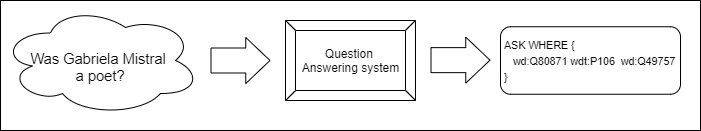
\includegraphics[scale=.5]{imagenes/1_intro/introQuestionAnsweringExample.png}
    \caption{Expected \SPARQL{} query example from a KGQA system.}
    \label{fig:introQAexample}
\end{figure}

The Query Template generator produces incomplete \SPARQL{} queries (which we call 
Query Templates) that contain \dquotesit{placeholders} in the position where entities are 
supposed to be (e.g. placeholders \texttt{<sbj\_1>} and \texttt{<obj\_1>} instead of entities 
\texttt{Q80871} and \texttt{Q49757} of the query shown in Figure~\ref{fig:introQAexample}). 
This module is built using the same model used to implement the baseline QAS. 
However, the training data is adapted to generate Query Templates instead of the complete 
query. This is achieved by removing the entities from the output \SPARQL{} queries included 
in the selected datasets such that the entities can rather be found by Entity Linking.

The role of the Entity Linking module is to recognize the relevant entities contained
in each question (e.g. identify that concepts \dquotesit{Gabriela Mistral} and \dquotesit{poet}
corresponds to the entities \texttt{Q80871} and \texttt{Q49757} in Figure~\ref{fig:introQAexample}) 
that are used to fill the Query Template. We implement various entity retrieval systems using 
one or more of the existing Entity 
Linking systems that have APIs available. The first variant is to use each EL system individually, 
which includes DBpedia Spotlight~\cite{EL:dbpedia-spotlight-MendesJGB11}, AIDA~\cite{EL:aida-tool-YosefHBSW11}, 
TAGME~\cite{EL:tagme-FerraginaS10}, and OpenTapioca~\cite{EL:opentapioca-Delpeuch19}. 
All of these systems, except for OpenTapioca, only work for DBpedia; therefore an 
extra mapping layer is implemented to map DBpedia entities to Wikidata entities. Two ensemble 
EL approaches are then proposed: one that prioritizes systems with higher Precision 
and another that implements a voting mechanism. We keep the variant that performs best 
according to the experiments that are explained in the \textit{Experimental results} subsection.

Additionally, a Slot Filling module is built by combining a Sequence Tagger model of the Flair 
library~\cite{seqlab:flair-AkbikBBRSV19} and a filling algorithm proposed in this work. Training 
the Sequence Tagger model requires building training data based on the selected datasets. 
Intuitively speaking, a Query Template may have multiple slots and multiple entities, where the 
Slot Filling module decides which entity should fill which slot (e.g. to infer that the concept 
\dquotesit{Gabriela Mistral} corresponds to the placeholder \texttt{<sbj\_1>}, therefore the 
entity \texttt{Q80871} should replace the occurrences of \texttt{<sbj\_1>} in the Query Template).

\subsection*{Experimental results}
\label{cap1:intro/contributions/expResults}
We conduct several experiments for validating each implemented module (Entity Linking, 
Slot Filling, and Query Template Generation) along with experiments over the defined 
benchmark for the end-to-end Question Answering process.

The Entity Linking systems are compared using Precision, Recall, and F1-score on the 
entities for each case on the dataset used for training. Testing is conducted over \QALDseven{} and 
our proposed dataset. The slot filling system is validated using Precision, Recall, and F1-score 
over the identified BIO labels (a common tagging format for sequence labeling tasks) over 
\LCQuADtwo{} and the mapped \DBNQA{} dataset. The query generator system is validated 
using BLEU score, Perplexity, and Accuracy over \LCQuADtwo{} and the mapped \DBNQA{} 
dataset. When training the query generator system, many split methods are tested according 
to the methodology proposed by Finegan-Dollak et al.~\cite{semPar:txt-to-sql-RadevKZZFRS18} for Text-to-SQL systems. 
The end-to-end Question Answering system is tested over all the datasets using the metrics 
described in the \textit{Benchmark on Question Answering over Wikidata} subsection.	
	%   Estructura del trabajo
	\section{Work Structure}
This worked is divided into the following chapters:

\begin{enumerate}
    \item In Chapter~\ref{cap2:theoFrame}, we describe the theoretical framework 
    enclosed on this work. This chapter covers concepts about what is the Semantic 
    Web, Information Extraction methods and how they relate with Semantic Web 
    technologies, Semantic Parsing applied on translating natural language to 
    \SPARQL, and the current state and challenges of the Question Answering over 
    Knowledge Graphs task.
    \item In Chapter~\ref{cap3:system}, we give an overview of the proposed Question 
    Answering system for this work. This includes a general explanation on the 
    pipeline proposed to generate a SPARQL query, and more specific details on how 
    each component is designed.    
    \item In Chapter~\ref{cap4:experimentalDesign}, we go into details about the 
    experiments we run on this work. We present the research questions we aimed to answer, 
    the baseline we compare our system with, and the metrics used to quantify the 
    performance of each system.    
    \item In Chapter~\ref{cap5:results}, we present the results derived from running the 
    proposed experiments. Aside from that, we include a brief discussion and analysis of 
    the results.    
    \item In Chapter~\ref{cap6:conclusions}, we summarize the conclusion of this work, 
    discuss its limitations and the future work regarding Question Answering over 
    Knowledge Graphs.
    
\end{enumerate}
	
\end{intro}
% Marco teorico
%   RDF y SPARQL
%   Entity Linking
%   Slot Filling
%   Redes Neuronales
%   Question Answering
\chapter{Theorical Framework}
	\label{cap2:theoFrame}
	% Semantic Web
	\section{Semantic Web}
\label{cap2:semWeb}

\subsection{Web of Data}
\label{cap2:semWeb/webOfData}
During the short history of the World Wide Web, we have greatly benefited from how its 
content has been increasing every day while serving multiple purposes. This vast amount of 
knowledge has become humanly impossible to traverse, so we rely on machines to 
process the content of documents automatically. As Hogan mentions, machines require the 
data to fulfill two primary requirements in order to be able to process them automatically 
in a meaningful way: to have a machine-readable structure and semantics~\cite{key:linked14-Hogan}. 
Unless a more \dquotes{formal} notion of structure and semantics is provided, machines can not 
be used to their full potential.

Various standards have emerged to partially structure the Web’s content, such as XML, CSV, 
or JSON. However, structured content without some semantics does not permit machines to do 
much more than split the content up by its delimiters and load its structure. Some other 
standards define semantic meaning for their structure, where some prominent examples are 
HTML, RSS or XML Schema (XSD), but often the semantics are defined in a human-readable way, 
for example, to describe how certain HTML elements should be rendered in a browser. Though 
these markup-based specifications provide a set of terms that often serve a singular purpose 
within the context of a given application, their interpretation tends to differ significantly 
for the respective consumer applications. 

The multiple purposes that standards like HTML can serve are not able to address some of the 
shortcomings of the current Web. Since content is often created to serve specific functionalities 
in the context of a given site, much of this content ends up not being directly reusable, 
high levels of redundancy appear or it cannot be integrated with other sites. In an effort 
to address these limitations, the Semantic Web was proposed.

The Semantic Web is designed as an extension of the current World Wide Web so as to enable 
the creation, sharing, and intelligent re-use of machine-readable content on the Web. The 
inception of the modern notion of the Semantic Web is founded on two major milestones: the 
original W3C recommendation of the first Resource Description Framework (\RDF{}) standard 
defining the core data model~\cite{key:oldrdf}, and the introduction of the vision for the 
Semantic Web outlined by Berners-Lee et al.~\cite{key:semwebsa}.

The vision of the Semantic Web can be represented through the Semantic Web Stack, first 
conceived by Berners-Lee et al., as seen in Figure~\ref{fig:semanticWebStack}. The lower levels describe the 
foundational elements of the Semantic Web which are aligned with the Web itself. First, 
the Web needs some standard to map from binary-streams and storage to textual information, 
so it relies on \textbf{Characters} from the standard Unicode character-set. Then, \textbf{Identifiers} 
respond to the main purposes of denoting any concept or concrete thing. The natural choice is to 
use Uniform Resource Identifiers (URI), which is the native standard for identification on 
the Web, or a recently adopted generalization of URI, Internationalized Resource 
Identifiers (IRI), which additionally support unescaped Unicode strings. The \textbf{Syntax} layer 
serves the objective of allowing machines to automatically parse content into its elementary 
components by defining syntaxes with formally defined grammars. For example, one of the most 
common syntaxes used to encode Semantic Web data is the Terse RDF Triple Language (Turtle) 
syntax~\cite{key:turtle}, based on the Notation3 (N3) syntax~\cite{key:n3}.

\begin{figure}[!h]
    \centering
    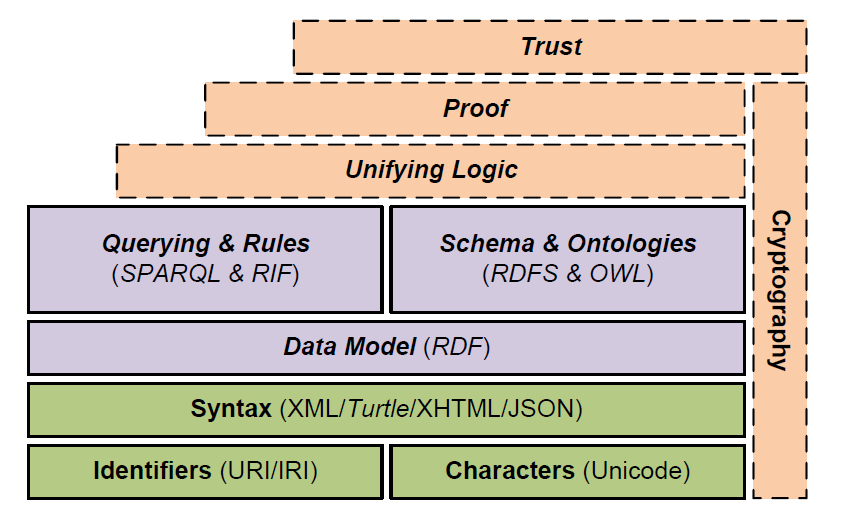
\includegraphics[scale=.65]{imagenes/2_theorical_framework/semanticWebStack.png}
    \caption{Semantic Web Stack~\cite{key:linked14-Hogan}}
    \label{fig:semanticWebStack}
\end{figure}

The next set of layers forms the core of the Semantic Web. The \textbf{Data Model} layer 
provides a canonical representation where machines can exchange machine-readable data in 
a generic framework. The core data-model for the Semantic Web is the Resource Description 
Framework (\RDF{})~\cite{key:rdfprimer}. In order to bring some meaning to the \RDF{} content, 
it requires formal languages whose meta-vocabulary complement the \RDF{} data-model by providing 
well-defined semantics. These languages correspond to the \textbf{Schema \& Ontologies} layer, 
where the RDF Schema (RDFS)~\cite{key:oldrdf} and Web Ontology Language (OWL)~\cite{key:owloverview, key:owl2rationale} 
standards are the essential languages integrated as part of the current Semantic Web. 
Eventually, the content described in \RDF{} needs to be processed by declarative querying 
and rules languages that serve many purposes, like generating results for user interfaces 
or inferring novel \RDF{} data. The \textbf{Querying \& Rules} layer is where the querying 
and rules standards for the Semantic Web are defined. In this case, the \textit{SPARQL Protocol 
and RDF Query Language}~\cite{key:sparql,key:sparql11protocol,key:sparql11} 
defines the querying standards and the Rule Interchange Format (RIF)~\cite{key:rifframework} 
defines the rules standards.

The top and side of the stack in Figure~\ref{fig:semanticWebStack} are layers yet to be realized. Though many 
proposals have been made in the research literature, no mature standards or tooling have 
emerged. The remaining top layers aim to combine the described low-level technologies into 
a unifying language to execute queries and rules over knowledge represented in \RDF{} 
(Unifying Logic), provide proofs to validate procedures or information used (Proof), and 
determine the trustworthiness of information sources (Trust). The Cryptography side layer 
is centered on cryptographic techniques for verifying and allowing access control mechanisms.

Providing more details on this broad overview of the Semantic Web, we start by focusing on 
how data is represented and how querying the content is described by any selected source. 
Then, in the following sections, we go deeper into understanding the Semantic Web data-model, 
\RDF{}, and its querying standard, \SPARQL{}.

\subsection{Resource Description Framework}
\label{cap2:semWeb/rdf}
The \textbf{Resource Description Framework} (\RDF{}) standard~\cite{key:rdfprimer} provides 
a data-model on the Semantic Web, which can be serialized using the Turtle syntax~\cite{key:turtle}. 
Having this data-model allows for any content framed in \RDF{} to be generically processed 
and indexed by external systems, whatever its topic or origin. The atomic elements that 
constitute the \RDF{} data-model are called \textbf{\RDF{} Terms}. \RDF{} does not follow the Unique 
Name Assumption (UNA), so two \RDF{} terms can refer to the same referent. The set of \RDF{} terms 
are divided into three disjoint subsets: URIs, Literals and Blank Nodes.

As mentioned previously, \textbf{Uniform Resource Identifiers} serve as identification for 
any resource. An example to identify the country Chile in DBpedia~\cite{KG:dbpedia} is 
the URI \url{http://dbpedia.org/resource/Chile}. A shorter version can be used 
by using the CURIE-style shortcuts~\cite{key:prefixes}, where a re-usable prefix can be 
defined: \texttt{@prefix dbr: <\url{http://dbpedia.org/resource/}>}. This way, the 
identifier of Chile can be abbreviated to \texttt{dbr:Chile}.

% note: ^ is \textasciicircum, ~ is \textasciicircum, \ is \textbackslash
\textbf{Literal} values represent lexical values and are divided into two categories. 
Plain literals are a set of plain strings, such as \texttt{\dquotes{Hello World}}, and can 
include an associated language tag, such as \texttt{\dquotes{Hello World}@en}. Typed 
literals are literals that include a datatype, such as 
\texttt{\dquotes{8}\textasciicircum\textasciicircum xsd:int}. Datatypes are identified by 
URIs (such as \texttt{xsd:int}) and borrow most of the datatypes defined for XML 
Schema~\cite{key:xsd}. Datatypes are often used for data validation or mapping.

\textbf{Blank Nodes} are used as existential variables that denote the existence of some 
resource without having to explicitly reference it using a URI or literal. The scope of a 
blank node is limited to the local \RDF{} document where it is defined, so it cannot be 
referenced elsewhere. In Turtle, blank nodes can be referenced explicitly with an 
underscore prefix \texttt{\_:bnode1} or implicitly in a variety of other manners.

\RDF{} terms are then combined together to form \RDF{} Triples. As its name suggests, a triple 
is a 3-tuple of \RDF{} terms. The three components of a triple are commonly called subject, 
predicate and object. \RDF{} triples can be seen as an atomic representation of a 
\dquotes{fact} or \dquotes{claim}, e.g. \dquotesit{Santiago is the capital city of Chile}. 
Typically each \RDF{} triple position fulfills a certain role: the subject is the primary 
resource that is being described (either a URI or a blank node), the predicate is the 
relation between the subject and the object (must be a URI), and the object is the value 
of the relation (any of the mentioned \RDF{} terms). For instance, we illustrate the Turtle 
representation of a set of \RDF{} triples from DBpedia in Listing~\ref{lst:dbpediaRdfExample}.

\begin{sparqlcode}[caption={Set of \RDF{} triples about Gabriela Mistral in DBpedia using Turtle syntax.},label={lst:dbpediaRdfExample}]
# PREFIX DECLARATIONS
@prefix dbr: <http://dbpedia.org/resource/>
@prefix dbo: <http://dbpedia.org/resource/>
@prefix dbp: <http://dbpedia.org/resource/>
@prefix rdfs: <http://www.w3.org/2000/01/rdf-schema#>

# RDF TRIPLES
dbr:Gabriela_Mistral rdfs:label "Gabriela Mistral"@en .
dbr:Gabriela_Mistral dbp:occupation dbr:Poet .
dbr:Gabriela_Mistral dbo:birthPlace dbr:Vicuña,_Chile .
dbr:Gabriela_Mistral dbo:awards dbr:Nobel_Prize_in_Literature .
dbr:Gabriela_Mistral dbo:awards dbr:National_Prize_for_Literature_(Chile) .
dbr:Vicuña,_Chile rdfs:label "Vicuna, Chile"@en .
dbr:Vicuña,_Chile dbo:populationTotal 25085 .
dbr:Vicuña,_Chile dbo:isPartOf dbr:Elqui_Province .
dbr:Vicuña,_Chile dbo:isPartOf dbr:Coquimbo .
dbr:Vicuña,_Chile dbo:country dbr:Chile .
\end{sparqlcode}

Listing~\ref{lst:dbpediaRdfExample} shows facts about Gabriela Mistral, a famous Chilean poet, 
and how those facts are structured as a set of \RDF{} triples, where each triple is separated by a 
dot symbol. The use of CURIE-style prefixes helps to simplify the content and make it easier to 
understand for a human reader~\cite{key:prefixes}. Moreover, Listing~\ref{lst:dbpediaShortRdf} 
shows how Turtle allows for abbreviating the content by grouping triples with common subjects 
(using the \squotestt{;} symbol) or predicates (using the \squotestt{,} symbol).

\begin{sparqlcode}[label={lst:dbpediaShortRdf},caption={Set of \RDF{} abbreviated triples about Gabriela Mistral in DBpedia.}]
...
# RDF TRIPLES
dbr:Gabriela_Mistral rdfs:label "Gabriela Mistral"@en ;
    dbp:occupation dbr:Poet ;
    dbo:birthPlace dbr:Vicuña,_Chile ;
    dbo:awards dbr:Nobel_Prize_in_Literature, dbr:National_Prize_for_Literature_(Chile) .
dbr:Vicuña,_Chile rdfs:label "Vicuña, Chile"@en ;
    dbo:populationTotal 25085 ;
    dbo:isPartOf dbr:Elqui_Province , dbr:Coquimbo ;
    dbo:country dbr:Chile .
\end{sparqlcode}

Given the triple-based structure of \RDF{} triples, it is possible to represent entire 
datasets as an \RDF{} graph, also known as a \textbf{Knowledge Graph} (KG): a directed labeled 
graph where subjects and objects are represented by nodes, and predicates are represented 
by the directed edges that bond two nodes. The \RDF{} graph of the example shown above can be 
drawn as in the diagram of Figure~\ref{fig:dbpediaGraphExample}, where by convention 
ellipses correspond to URIs or blank nodes, and rectangles symbolize literals.

\begin{figure}[!h]
    \centering
    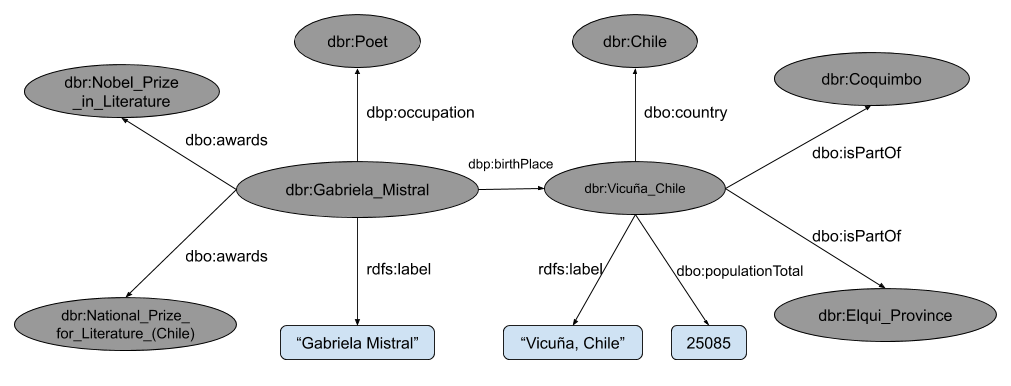
\includegraphics[scale=.55]{imagenes/2_theorical_framework/exampleDbpediaGraph.png}
    \caption{\RDF{} graph representing facts about Gabriela Mistral from Listing~\ref{lst:dbpediaRdfExample}.}
    \label{fig:dbpediaGraphExample}
\end{figure}

Besides \RDF{} triples and \RDF{} graphs, \RDF{} standards provide a rich set of built-in 
vocabulary terms under a core \RDF{} namespace, which helps to standardize frequently used 
\RDF{} patterns. One popular term is \texttt{rdf:type}, which helps to assign resources 
sharing certain commonalities into \textbf{classes}. For example, we can denote 
\texttt{dbr:Vicuna\_Chile} as a city by combining it with the predicate \texttt{rdf:type} 
and the object \texttt{dbr:City}. Another example is the term \texttt{rdfs:label} that 
comes from RDF Schema~\cite{key:rdfsold}, which provides other resources for describing 
relations such as \textbf{subproperties} or \textbf{subclasses}. Though our work is not 
focused on the use of the Web Ontology Language (OWL)~\cite{key:owl2rationale, key:owloverview}, 
it is worth mentioning that it also adds a wealth of new vocabulary to describe new 
relations between resources like equivalences, disjointness, inverse properties, among others.

Ultimately, there are numerous syntaxes for writing \RDF{} apart from Turtle~\cite{key:turtle}, among 
which we can name RDF/XML~\cite{key:rdfxml}, N-Triples~\cite{key:testcases}, RDFa~\cite{key:rdfa11p, key:rdfa}, 
and JSON LD~\cite{key:jsonld}. However, no matter what syntax is chosen, every one is 
represented in the same \RDF{} data model; thus it is possible to convert any \RDF{} content 
in one syntax to another while keeping the same \RDF{} data.

\subsection{SPARQL Query Language}
\label{cap2:semWeb/sparql}
The \textbf{SPARQL} protocol defines how \SPARQL{} queries retrieve results over the \RDF{} 
data-model~\cite{key:sparql11protocol}. These standards became W3C Recommendations in 
2008~\cite{key:sparql} and then were extended in 2013 in the SPARQL 1.1 version~\cite{key:sparql11} 
superseding the previous W3C Recommendations. Some \SPARQL{} query features and keywords are similar 
to the ones found in the Structured Query Language (SQL), though \SPARQL{} is designed for interacting 
with \RDF{} data.

\begin{sparqlcode}[%
    caption={\SPARQL{} query for getting awards won by people who were born in Vicuña.},
    label={lst:dbpediaSparqlExample}]
# PREFIX DECLARATIONS
PREFIX dbr: <http://dbpedia.org/resource/>
PREFIX dbo: <http://dbpedia.org/ontology/>
# DATASET CLAUSE
FROM <http://dbepdia.org/data/Gabriela_Mistral.ttl>
# RESULT CLAUSE
SELECT ?people ?award
# QUERY CLAUSE
WHERE {
    ?people dbo:birthPlace dbr:Vicuña,_Chile ;
        dbo:award ?award .
}
# SOLUTION MODIFIERS
LIMIT 2
\end{sparqlcode}

There are five main components that describe a \SPARQL{} query. First, \textbf{Prefix Declarations} 
serve as shortcuts for later in the query, similar to the Turtle shortcuts. Following prefixes, 
the \textbf{Dataset Clause} allows for specifying one or more \RDF{} graphs over which the query 
should be executed. When no dataset clause is specified, query patterns are matched against the 
default graph which usually corresponds to all of the data loaded and indexed. The 
\textbf{Result Clause} indicates what type of query is being executed and what results are expected. 
The most relevant part is the \textbf{Query Clause}, where the query patterns to match against the 
data are specified and used to generate variable bindings. Finally, the \textbf{Solution Modifiers} 
permit to order, slice or paginate the results. Note that the only mandatory part is the result 
clause, though most queries also include at least one query clause. An example of a \SPARQL{} query is 
represented in Listing~\ref{lst:dbpediaSparqlExample}, where we are looking for which awards 
people who were born in Vicuña have won.

For example, if the \RDF{} triples shown in Listing~\ref{lst:dbpediaRdfExample} were contained in the 
\RDF{} graph \texttt{<\url{http://dbpedia.org/data/Gabriela\_Mistral.ttl}>}, the results 
expected from the \SPARQL{} query in Listing~\ref{lst:dbpediaSparqlExample} would be as shown 
in Table~\ref{table:dbpediaExampleResults}.

\begin{table}[h!]
    \centering
    \begin{tabular}{ |c|c| }        
        \hline
        ?people & ?award \\ 
        \hline
        dbr:Gabriela\_Mistral & dbr:Nobel\_Prize\_in\_Literature \\
        dbr:Gabriela\_Mistral & dbr:National\_Prize\_for\_Literature\_(Chile) \\
        \hline
    \end{tabular}
    \caption{Results from \SPARQL{} query example in Listing~\ref{lst:dbpediaSparqlExample}.}
    \label{table:dbpediaExampleResults}
\end{table}

There are four types of \SPARQL{} queries, which are defined by the first keyword used in the 
\textit{Result Clause}. The example shown above is a \texttt{SELECT} query, which requests a list 
of bindings for variables specified in the \textit{Query Clause}. Since a \texttt{SELECT} query 
returns duplicate results by default, it can include either the \texttt{DISTINCT} keyword to filter 
duplicate results, or the \texttt{REDUCED} keyword that may allow duplicates such that the engine 
can choose whatever it deems to be more efficient. An \texttt{ASK} query returns a boolean value 
indicating whether or not the query’s results are non-empty. A \texttt{CONSTRUCT} query provides 
an \RDF{} template with placeholders to be filled later, thus returning an \RDF{} graph according to 
those inserted variables. The last type is the \texttt{DESCRIBE} query, which provides an \RDF{} 
description for a particular \RDF{} term. For this work we only focus on \texttt{SELECT} and 
\texttt{ASK} type queries.

Knowing how to define the content inside a \textit{Query Clause} is crucial in order to specify what results 
a \SPARQL{} query should return. There are many core features defined over the basic graph patterns 
that are used to create complex query patterns in query clauses. Among these patterns, we highlight 
the \texttt{FILTER} keyword that serves to establish conditions that a query solution should match. 
These conditions can be constructed from a broad arsenal of tools: arithmetic operators and 
comparators, built-in functions, casting, boolean connectives and even user-defined functions. 
We also mention the \texttt{UNION} operator, that allows joining results from two groups of query 
patterns. Another important feature is the \texttt{OPTIONAL} feature, which allows for matching 
data if available (if not, the corresponding result is still returned, where the variables 
exclusive to the \texttt{OPTIONAL} clause are left unbound).

After retrieving results from the \textit{Query Clause}, such results can be divided or modified. 
The \texttt{ORDER BY} operation sorts results in ascending (\texttt{ASC}) or descending (\texttt{DESC}) order based 
on one or more variables; and the \texttt{LIMIT} keyword restricts the amount of results to return. 
Finally, the \texttt{OFFSET} clause allows the query to skip a certain number of results.

Besides the basic operations provided by the original \SPARQL{} standard, the later update to 
SPARQL 1.1~\cite{key:sparql11} brought a wide-range of new features that increase the expressiveness 
and capabilities of this query language. Some core additions are property paths, aggregation, 
binding variables, subqueries, updates, new format outputs (CSV, TSV, JSON), among others. 
For this work we want to highlight the use of \textit{property paths} and \textit{aggregation} 
that will be often used. \textit{Property paths} allow the user to match paths of arbitrary 
length in an \RDF{} graph using regular expressions. \textit{Aggregation} techniques include 
operations like count, max, min, sum, etc.; and can be applied over query results grouped 
by common terms.

Though many other \SPARQL{} features are left to be mentioned, we focused on the features described 
above since those are the important ones for the development of this work.

\subsection{Linked Open Data Cloud}
\label{cap2:semWeb/linkedData}
Having briefly mentioned some core components of the Semantic Web, we have scratched just a tiny 
portion of what the Semantic Web concept means, and how it can be deployed on the Web. Most of 
what defines the use of the Semantic Web on the Web itself resides in understanding 
\textbf{Linked Data}. The early attempts to publish \RDF{} on the Web tended to produce large dumps 
of data rarely interlinked with other \RDF{} datasets and using different conventions. These issues 
ended up leaving entire isolated islands of \RDF{} datasets that were difficult to access and with 
little chance of being discovered by other communities. Therefore, \textit{Linked Data} emerged as 
a set of principles and best practices~\cite{key:ldprinciples} to provide an environment where 
Semantic Web standards can be effectively deployed on the Web.

The four Linked Data principles arise from the Web Design Issues document published by 
Berners-Lee~\cite{key:ldprinciples}. According to this document, these principles are: (1) use URIs 
as names for things, (2) use HTTP URIs so those names can be looked up, (3) return useful 
information upon lookup of those names, and last (4) include links by using URIs that dereference 
to remote documents. 

Besides these principles, there is an emphasis on publishing data that can be easily processed, 
reused and exchanged between machines. As an approach to bootstrap Semantic Web publishing, 
a 5-star system~\cite{key:ldprinciples} was promoted to describe the quality of published \RDF{} data. 
Each star corresponds to one of the following considerations: (1) publish data under an open license, 
(2) publish structured data, (3) use non-proprietary formats, (4) use URIs to identify things, and 
(5) link the published data to other data.

A community project named \dquotesit{Linking Open Data}, supported by W3C and inspired by the growth 
in Open Data, emerged to promote these Linked Data principles~\cite{key:ldbook}. The community 
project aims to introduce the benefits of Semantic Web technologies to the Open Data movement and 
to bootstrap the Web of Data by including many emerging open datasets. The community published 
guidelines are based on the core principles mentioned before. Among those guidelines, the main 
ones are:

\begin{itemize}
    \item \textbf{Dereferencing practices}: describes how to identify and perform lookups 
    for either entities or documents. This includes recommendations on indirect URIs to signify 
    distinctions on a HTTP level or providing as detailed an \RDF{} description as possible when 
    dereferencing resources. 
    \item \textbf{Linking Aliases}: allow the use of multiple URI aliases that refer to the same 
    thing. For example, \texttt{owl:sameAs} links can be used to specify equivalence between 
    resources in different datasets.
    \item \textbf{Describing Vocabularies Terms}: promotes the shared use of common vocabularies 
    of class and property terms. A common example is to use FOAF to describe people.
    \item \textbf{Provision of SPARQL Endpoints}: though not required, providing a \SPARQL{} endpoint 
    for a given Linked Data site gives consumers a single-point-of-access to query over the merge 
    of contributions on that site.
\end{itemize} % TODO: check why itemize put so much space between items (removing following section line reduces the space to normal)

Based on these standards and guidelines, the \textbf{Linking Open Data Cloud}, a set of more than 
300 different interlinked \RDF{} datasets, has been constantly growing and including a wider range of 
topics. Some of the most relevant datasets are DBpedia~\cite{KG:dbpedia}, whose content is mostly 
based on Wikipedia articles, Freebase~\cite{KG:freebase}, a dataset previously supported by Google, 
and Wikidata~\cite{KG:wikidata}, a large dataset supported by its community. Our work is mainly 
focused on the latter knowledge graph, which we will introduce in the next section.

\subsection{Wikidata}
\label{cap2:semWeb/wikidata}
As described by Vrandečić and Krötzsch~\cite{KG:wikidata}, \textbf{Wikidata} is a free 
collaborative Knowledge Graph founded by the Wikimedia Foundation\footnote{\url{https://wikimediafoundation.org/our-work/wikimedia-projects/}} 
in October 2012. Given the constant growth of its sister project Wikipedia, one of the most 
popular online encyclopedias, Wikidata is introduced as a new multilingual 
\dquotesit{Wikipedia for data}. 

Despite Wikipedia’s rich amount of data, consisting of more than 30 million articles in at least 
287 languages, it started to face serious limitations in terms of providing data easily to the 
community~\cite{KG:wikidata}. There was the lack of direct access through query services or 
downloadable data exports, the same information often needed to be manually maintained in the 
same articles across many languages and across many articles within a single language, among 
others limitations. Wikidata aims to overcome many of Wikipedia’s limitations by managing its 
data centrally.

Wikidata offers many features that make it an attractive and potentially useful resource for 
sharing information and connecting communities. Some aspects to consider about Wikidata are:

\begin{itemize}
    \item \textbf{Openly editable}: allows any user to extend and edit the stored information.
    \item \textbf{Community control}: contributor community control that not only supervises the 
    data being published but also the schema of the data. 
    \item \textbf{Plurality}: though many facts can be disputed or be uncertain, Wikidata provides 
    mechanisms to organize conflicting data for coexisting together.
    \item \textbf{Secondary data}: gathers facts published in primary sources including references 
    to these sources.
    \item \textbf{Multilingual data}: all data have universal meaning and most of it is not tied 
    to a single language. There is only one universal version of Wikidata.
    \item \textbf{Easy access}: data published under liberal legal terms are made  easily 
    accessible through web services, allowing the widest possible reuse.
    \item \textbf{Continuous evolution}: Wikidata grows with its community of editors and 
    developers, so new features are constantly being added.
\end{itemize}

Wikidata has its own data model but further offers exports that follow the Semantic Web 
standards~\cite{key:wikidataErxlebenGKMV14}. To identify items, Wikidata provides unique IDs, 
which are highly reusable and provide unambiguous definitions that do not depend on language 
labels. The same example of the entity Chile mentioned before is now represented in Wikidata as 
\texttt{\url{http://www.wikidata.org/wiki/Q298}}. 

\begin{sparqlcode}[%
    caption=Set of RDF triples about Gabriela Mistral in Wikidata., 
    label=lst:wikidataRdfExample]
# PREFIX DECLARATIONS
@prefix wd: <http://wikidata.org/wiki/>
@prefix wdt: <http://wikidata.org/prop/direct/>
@prefix p: <http://wikidata.org/prop/>
@prefix pq: <http://wikidata.org/prop/qualifier/>
@prefix rdfs: <http://www.w3.org/2000/01/rdf-schema#>

# RDF TRIPLES
# Gabriela Mistral
wd:Q80871 rdfs:label "Gabriela Mistral"@en ;
    wdt:P106 wd:Q49757 ;
    wdt:P19 wd:Q201007 ;
    wdt:P166 wd:Q37922, wd:Q860699 .
# Vicuna
wd:Q201007 rdfs:label "Vicuña"@en ;
    p:P1082 _:population2017 ;
    wdt:P131 wd:Q721224 ;
    wdt:P17 dbr:Chile .
_:population2017 pq:P1082 25085
# Elqui Province
wd:Q721224 wdt:P131 wd:Q2121 .
\end{sparqlcode}

Since some facts cannot be directly expressed by simply using the property-value convention, 
like the population of Chile across different years, Wikidata also provides additional 
subordinate property-value pairs called \dquotesit{qualifiers}. \textbf{Qualifiers} can be used 
to state contextual information such as validity time or ternary relations (e.g. cast members of 
a movie with their role). Another way to understand qualifiers is by looking at Wikipedia 
infoboxes which have a similar data representation.

\begin{figure}[!h]
    \centering
    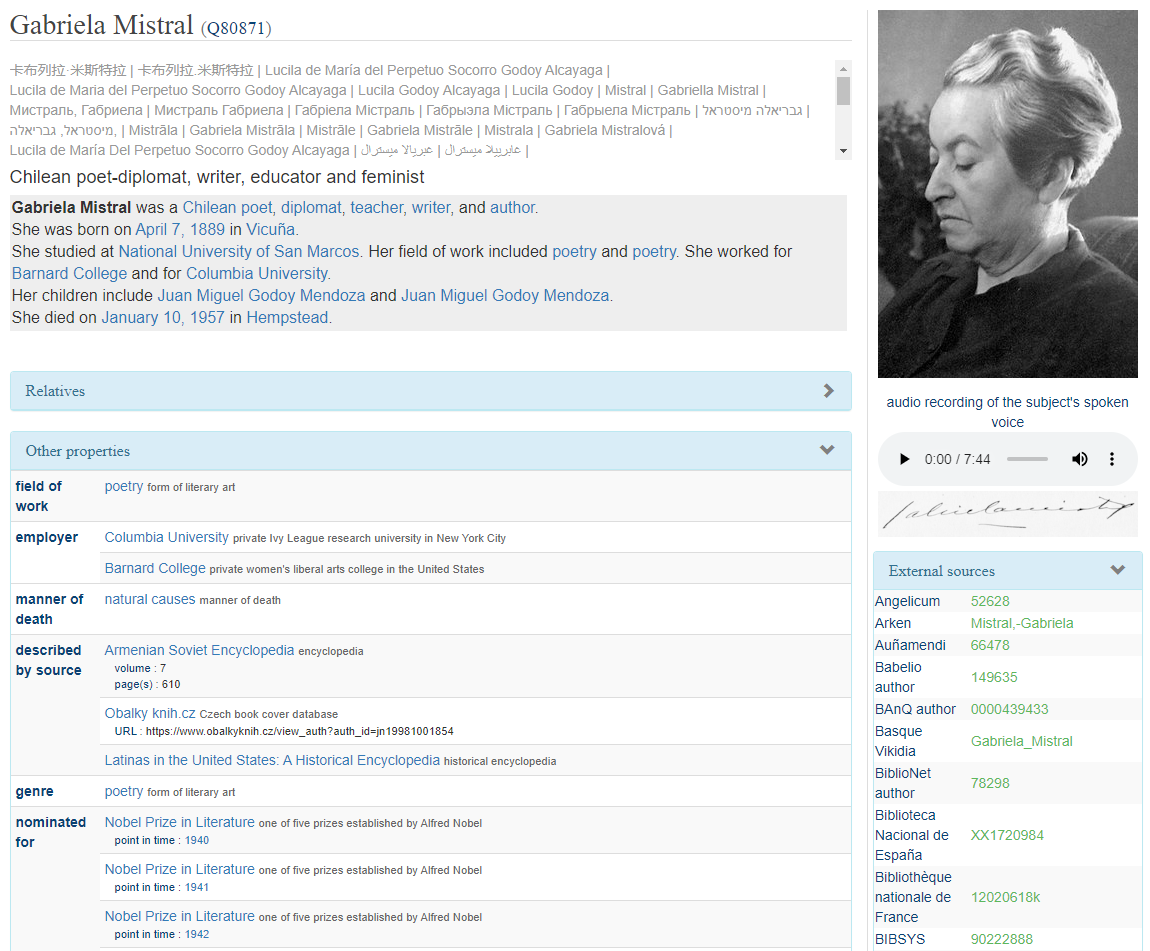
\includegraphics[scale=.5]{imagenes/2_theorical_framework/wikidataReasonatorExample.PNG}
    \caption[Example of an external application of Wikidata using Reasonator.]{Example of an external application of Wikidata using Reasonator\footnotemark.}
    \label{fig:wikidataReasonator}
\end{figure}

\footnotetext{\url{https://reasonator.toolforge.org/?&q=80871}}

For a better understanding, let us recall the same data about Gabriela Mistral, but now using 
Wikidata resources, as shown in Listing~\ref{lst:wikidataRdfExample}. Since different knowledge 
graphs do not necessarily represent the same information in the same way, we can appreciate slight 
differences like how the city Vicuña is described. In this case, Vicuña is not directly represented 
as part of Coquimbo but instead only the Elqui Province. Nevertheless, both representations are 
intrinsically correct since both are portraying the same fact. Another difference is the use of 
a Wikidata property qualifier to denote that the population for Vicuña shown in 
Listing~\ref{lst:wikidataRdfExample} is the population of 2017, in contrast to the DBpedia 
representation, shown in Listing~\ref{lst:dbpediaShortRdf}, which does not show that fact.

Ultimately, the data in Wikidata lends itself to numerous applications on very different levels 
of data integration. Wikidata provides many language labels and descriptions for many terms in 
different languages, which allows any service to present and/or or translate information for 
various audiences. Some applications are built to access Wikidata’s data more conveniently and 
effectively. One example is illustrated by Figure~\ref{fig:wikidataReasonator}, showing 
information about Gabriela Mistral retrieved by the data browser 
\textit{Reasonator} using the Wikidata API. Additionally 
applications can be enriched with information provided by Wikidata, such as how Google Maps 
uses Wikidata’s geographical labels to enhance its application interface. 

On a more advanced level, many research analyses can be performed over the information in 
Wikidata in order to derive new insights beyond its surface data. A couple of potential examples 
are analyses using logical reasoning to understand intrinsic meaningful relationships among 
entities, or statistical evaluations over the data to analyze biases like the ones that involve 
language coverage~\cite{key:wikidataHale13} or gender balance~\cite{key:socialWikidataWagner16}. 
Wikidata is already an important platform and has the potential to be a major resource for both 
researchers and developers~\cite{wikidata:GeneWikiInitiative, wikidata:RiseWikidataVrandecic6682924}.
	
	% Information Extraction
	\section{Information Extraction}
\label{cap2:theoFrame/infExtr}
\subsection{Information Extraction methods with Semantic Web technologies}
\label{cap2:theoFrame/infExtr/methods}
As the Semantic Web aims to make structured data available enabling high levels of 
automation, there are still some challenges regarding the increasing demand for information. 
There is still a gap between the coverage of structured and unstructured data on the 
Web~\cite{infExtr:PolleresHHD10}. However, making high-quality annotations on unstructured 
data is not a trivial task because it requires processing vast amounts of information that 
is constantly changing. 

Thus, automatic techniques for extracting and annotating information have gotten more 
attention in the context of the Semantic Web. As described by Martinez et. al., Information 
Extraction (IE) refers to the automatic extraction of implicit information from unstructured 
or semi-structured sources~\cite{infExtr:MartinezHL19}. IE methods are used to identify 
entities, concepts and/or semantic relations implicit in an input source, typically a text 
in natural language. 

Many systems have been developed to automate the extraction or enrichment of Semantic Web 
resources such as ontologies, knowledge graphs, etc. These systems are often based on 
Information Extraction methods which usually rely on techniques from areas such as Natural 
Language Processing, Machine Learning and Information Retrieval. 

The combination of tools from the Semantic Web and Information Extraction areas presents two 
perspectives: using Information Extraction to populate the Semantic Web, or using Semantic 
Web resources to improve Information Extraction processes. In this work we focus on the last 
perspective mentioned, in particular how to extract and link entities over unstructured input 
sources (such as natural language questions).

An entity is understood as an atomic element within a Semantic Web knowledge base or ontology. 
Entity Extraction \& Linking (EEL) is then the task of identifying mentions in a text or 
document, and linking them as entities to one or more reference knowledge graphs. EEL is 
typically divided into two main steps: a recognition stage where relevant named entities are 
identified, and a disambiguation stage, where entities are mapped to candidate resources in 
the knowledge graph and subsequently ranked. Entity extraction often uses off-the-shelf Named 
Entity Recognition (NER) tools to recognise relevant entities. After extraction, Entity 
Linking follows, where the disambiguation of the spotted mentions links each mention to an 
identifier in a target knowledge graph, and may include a score or weight calculation that 
denotes the confidence or support over the output annotations. We now discuss the Entity 
Linking process in more detail.

\subsection{Entity Linking}
\label{cap2:theoFrame/infExtr/entityLinking}
Entity Linking is the task of linking mentions in text to their corresponding entities in a 
knowledge graph (e.g. Wikipedia, Wikidata, DBpedia)~\cite{EL:survey-WuHH18}. Aside from 
extracting entities from a knowledge graph, a disambiguation step is also needed. For example, 
for the question \textit{“Has Claudio Bravo played for Manchester City FC?”}, Entity Linking 
with respect to Wikidata should link the mention \textit{“Claudio Bravo”} to the Chilean 
football goalkeeper Claudio Bravo (wd:Q313161) instead of the Chilean painter Claudio Bravo 
(wd:Q491787), given the context of the sentence (a person playing in a football club). Some 
applications of Entity Linking involve fields such as information 
retrieval~\cite{infExtr:CornoltiFCRS16, infExtr:BlancoOM15, infExtr:BollegalaMI07} knowledge 
fusion~\cite{infExtr:DongGHHMSZ15, infExtr:BohmFHLMNEHHS12}, or knowledge base 
population~\cite{infExtr:RaoMD13, infExtr:DredzeMRGF10, infExtr:FreedmanMM17}.

Commonly, the entity linking process is divided into three modules: candidate entity 
generation, candidate entity disambiguation and linking the result. A formal description of 
Entity Linking according to Wu and He~\cite{EL:survey-WuHH18} is the following: Given a set of 
documents $d=\{d_1,d_2,\ldots\}$ and a knowledge base $K$, we can get a mention set 
$M=\{m_1, m_2,\ldots\}$ using a Named Entity Recognition tool. For each $m_i \in M$, we can 
get a candidate set $C=\{c_1, c_2,\ldots\}$ from a knowledge base. The goal of Entity Linking 
is to choose an entity from $c \in C$ for each mention $m \in M$. If $score(m,c)$ is below 
$\tau$ ($\tau$ is a threshold) for all $c \in C$, then the target entity of m is 
\textit{Not In Lexicon} (NIL); otherwise, $m$ will be linked to $c'$ such that 
$score(m,c')=max\{score(m,c) \mid c\in C \}$. Figure~\ref{fig:entitylinkingGeneralModel} shows a 
general model including each phase and the formal description mentioned.

\begin{figure}[!h]
    \centering
    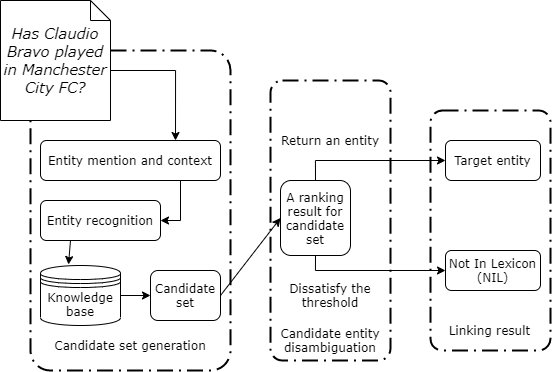
\includegraphics[scale=.5]{imagenes/2_theorical_framework/information_extraction/entityLinkingModel.PNG}
    \caption{A general model of Entity Linking based on Wu and He~\cite{EL:survey-WuHH18}}
    \label{fig:entitylinkingGeneralModel}
\end{figure}

The first module selects the candidate entities for each mention identified in the text and 
finds related entities in the knowledge base. For example, \textit{Claudio Bravo} is related 
to the entities \textit{Claudio Bravo (football goalkeeper)} and \textit{Claudio Bravo (painter)}.

The second module ranks the candidate entities by combining different features of 
entities and assigning scores to each candidate. Some features could be entity popularity, 
entity type, similarity between names or context in the query, topic similarity and a 
combination of several features. In the example, \textit{Claudio Bravo (football goalkeeper)} 
should have a higher score than \textit{Claudio Bravo (painter)} due to the football-related 
context of the sentence. 

The last module selects the target entity for each mention according to the ranking derived 
from the previous module. The candidates with the highest score per mention are selected 
among the candidates whose scores are above the threshold. If scores from all candidates are 
below the threshold, some systems return a NIL clustering~\cite{infExtr:ji2010overview}, 
although we will work with systems that directly discard results that do not satisfy the 
threshold.

There are various existing methods for addressing candidate entity generation and 
disambiguation. The methods for candidate entity generation can be divided into methods 
based on dictionaries~\cite{infExtr:ZhangSTW10, infExtr:HanSZ11}, 
direct search~\cite{infExtr:McNameeMLOD11, infExtr:DredzeMRGF10} and 
probabilistic methods~\cite{infExtr:ganea2016, infExtr:PanCHJK15}. On the other hand, the 
methods for candidate entity disambiguation can be divided into methods based on 
similarity computation~\cite{infExtr:Cucerzan07, infExtr:BunescuP06}, 
machine learning~\cite{infExtr:ganea2016, infExtr:ZhangSTW10} 
and graphs~\cite{infExtr:GongFLSH17, infExtr:HanSZ11}.

One of the main difficulties in Entity Linking is the high ambiguity of entity mentions, 
which make it more difficult to understand the meaning of entity mentions. These ambiguities 
include polysemies, which refer to mentions that correspond to many entities (e.g. 
\textit{Claudio Bravo}) or multiword synonyms, which refer to entities that may have many 
kinds of surface forms (e.g. \textit{Manchester City FC} is also known as \textit{The Citizen} 
or \textit{The Sky Blues}). Another problem happens when selecting entities in the linking 
results phase since the threshold is selected manually and can lead to the problem that 
correct targets can be below the threshold, thus being discarded.

Entity linking evaluation criteria are usually based on Precision, Recall and 
F1-score. For each of these metrics there is a micro measure and a macro 
measure~\cite{entlin:CornoltiFC13}. The macro measure gives equal importance to each 
document since it first calculates the relevant measure over each document, and then 
calculates the arithmetic average. On the other hand, the micro measure considers all 
mentions as part of one document when calculating the relevant measure, thus giving more 
importance to documents with more mentions. The following equations represent the micro and 
macro measures of Precision and Recall:
% E --> G, G --> S
\begin{align*} 
    Precision_{micro} = \frac{|S \cap G|}{|S|} \\
    Recall_{micro} = \frac{|S \cap G|}{|G|} \\
    Precision_{macro} = \frac{\sum_{i=1}^{|D|} \frac{|s_i \cap g_i |}{|s_i|}}{|D|} \\
    Recall_{macro} = \frac{\sum_{i=1}^{|D|} \frac{|s_i \cap g_i |}{|g_i|}}{|D|}
\end{align*}
\noindent where $D$ represents a document containing a number of texts, $G$ is the set of annotated 
entities that should be linked in a document ($g_i$ is the equivalent for each document), 
$S$ the set of linked entities generated by a system in a document ($s_i$ is the equivalent 
for each document). The precision is the ratio of entities correctly linked to a Knowledge 
Graph over the linked entities generated by a system, while the recall is the ratio of 
entities correctly linked to a knowledge graph over the entities that should be correctly 
linked. Then, the F1-score is a measure that combines Precision and Recall as two 
interacting values and is calculated with the following formula (based on the harmonic 
mean of both measures):

\[
    F1_x = 2 \frac{Precision_x \cdot Recall_x}{Precision_x + Recall_x}
\]
\noindent where $x$ corresponds to the micro or macro version of the F1-score. Aside from Precision, 
Recall and F1-score, some systems also include an Accuracy measure that includes NIL entities, 
though we will not consider this metric in our evaluations as NIL entities in questions 
cannot generate results for queries.

There are many datasets used for evaluation such as KORE50~\cite{entlin:HoffartSNTW12}, 
AIDA-CoNLL~\cite{EL:aida-HoffartYBFPSTTW11}, NEEL~\cite{entlin:RizzoBPV15}, and 
OKE2016~\cite{entlin:Plu0T16}, which can be evaluated over knowledge bases such as Wikipedia, 
DBpedia~\cite{KG:dbpedia}, and YAGO~\cite{KG:yago}. To the best of our knowledge, there is 
no dataset for evaluating Entity Linking over Wikidata, but since Wikidata, DBpedia and 
Wikipedia are all interlinked, we can use datasets with labels for any such resource.

In this work we will use several Entity Linking systems that we will briefly describe later. 
The criteria to choose these systems were: 

\begin{enumerate}
    \item have a public API available that allows at least 10,000 requests per day; 
    \item have references/papers explaining how the system functions; and 
    \item work over either Wikipedia, Wikidata, DBpedia or YAGO. 
\end{enumerate}

Given these criteria, the selected systems are: \textit{DBpedia Spotlight}, \textit{AIDA}, 
\textit{TAGME} and \textit{OpenTapioca}.

% TODO: check EL explanations
\subsubsection{DBpedia Spotlight}
\label{cap2:theoFrame/infExtr/entityLinking/dbpediaSpotlight}
DBpedia Spotlight~\cite{EL:dbpedia-spotlight-MendesJGB11} is a system that automatically 
annotates text documents with DBpedia URIs. The system allows users to configure annotations 
to their specific needs through the DBpedia Ontology and quality measures provided by the 
system. Their approach is divided into four phases.

The \textbf{spotting stage} identifies the phrases in a sentence that may contain a mention 
of a DBpedia resource. Before performing the spotting process, the system builds a lexicon 
of labels extracted using a graph of labels, redirects and disambiguation pages in 
DBpedia. The labels of DBpedia resources are created from Wikipedia page titles, which are 
seen as community-approved surface forms. Redirects to URIs indicate synonyms or alternative 
surface forms (including common misspellings and acronyms) whose labels also become surface 
forms. Disambiguation pages provide links from ambiguous surface forms to the resources they 
potentially link to. The resulting collection of surface forms composes the set of labels for 
the target resources.

As an additional resource for the later disambiguation stage, a collection of occurrences for 
each resource based on wikilinks (page links in Wikipedia associated with one resource) is 
stored as a document in a Lucene\footnote{\url{http://lucene.apache.org}} index.

A \textbf{candidate selection} is then employed to map resource names to candidate 
disambiguations spotted in the previous phase. The DBpedia Lexicalization dataset is used to 
determine candidate disambiguations for each surface form. This phase aims to reduce the 
number of disambiguation possibilities keeping a trade-off between time performance and 
system recall. 

Following candidate selection is the \textbf{disambiguation stage}, where the system uses 
the context gathered from surface forms to choose the best choice amongst candidates. 
DBpedia resource occurrences are modeled in a Vector Space Model (VSM)~\cite{infExtr:SaltonWY75} 
where each DBpedia resource is a point in a multidimensional space of words. The \textit{Term 
Frequency} (TF) weight and the \textit{Inverse Candidate Frequency} (ICF) weight are 
used to score each candidate. 

The TF weight represents the relevance of a word for a given resource. The ICF weight is 
proposed given that the standard \textit{Inverse Document Frequency} (IDF) 
weight~\cite{infExtr:Jones04} only identifies the global importance for a word, and thus 
fails to capture the importance of a word for a specific set of candidate resources. Instead, 
the ICF weight aims to weight words based on their ability to distinguish between candidates 
for a given surface form. The intuition behind the ICF formula is that the discriminative power 
of a word is inversely proportional to the number of DBpedia resources it is associated with. 

Having the VSM representation of DBpedia resources with $TF \ast ICF$ weights, the 
disambiguation process is performed by ranking candidate resources using the cosine 
similarity score between their context vectors and the context surrounding the surface form.

Finally, annotations can be customized through \textbf{configuration parameters} in order to 
tune parameters to a specific task. The offered configuration parameters can be used to 
allow/deny URIs with some classes or its subclasses, set a required minimum of inlinks, 
establish thresholds to prioritise resources relevant to the topic, reduce highly ambiguous 
resources, and configure a disambiguation confidence to keep a good trade-off between avoiding 
incorrect annotations and losing correct annotations.

A web-service\footnote{\url{https://www.dbpedia-spotlight.org/}} is available for integration with 
external web processes. The service is implemented through RESTful and SOAP web services for 
the annotation and disambiguation processes, and supports various output formats (HTML, XML, 
JSON or XHTML+RDFa).

\subsubsection{AIDA}
\label{cap2:theoFrame/infExtr/entityLinking/aida}
The Accurate Online Disambiguation of Named Entities (AIDA)~\cite{EL:aida-HoffartYBFPSTTW11,EL:aida-tool-YosefHBSW11} 
is an online tool that performs entity detection and disambiguation over the YAGO Knowledge 
Graph. The system's approach combines the use of a Named Entity Recognition (NER) tool with a 
graph-based mapping. 

The system automatically detects mentions using the Stanford NER 
Tagger\footnote{\url{https://nlp.stanford.edu/software/CRF-NER.shtml}} based on a Conditional Random 
Fields (CRF) Classifier~\cite{entLin:FinkelGM05}. Their approach uses Gibbs sampling to identify 
non-local structures while preserving tractable inference by simulated annealing in place of 
Viuterbi decoding in sequence models. They use this technique to improve an existing CRF-based 
information extraction system with long-distance dependency models.

The collection mapping relies on a graph constructed with mentions and their candidate entities 
as nodes and two types of edges: \textit{mention-entity edges} and \textit{entity-entity edges}. 
The \textbf{mention-entity edges} are weighted edges between mentions and their candidates 
entities (one edge per candidate) and represent the similarity between the context of each node. 
The \textbf{entity-entity edges} are weighted edges between different entities and represent the 
coherence, i.e. the semantic relatedness between both nodes.

The \textit{similarity} between a mention and a candidate entity is defined as the linear 
combination of the \textit{prominence} of an entity and the \textit{context similarity} between 
a mention and a candidate entity. The \textbf{prominence} (or popularity) of an entity is 
calculated using the frequency of Wikipedia-based link href anchor texts and links referencing 
the entity. The \textbf{context similarity} is calculated in different ways for a mention's 
context and an entity's context. 

The context of a mention simply considers all tokens in the document as the 
context~\cite{infExtr:ThaterFP10}. For the context of an entity, the system considers entity 
keyphrases, which are pre-computed phrases derived from link anchors in Wikipedia articles that 
entities connect to~\cite{infExtr:ThaterFP10}. These include phrases in the entity article that 
contain category names, citation titles, external references or titles of incoming links. This 
process forms a keyphrase set $KP(e)$ for each entity $e$. 

The \textit{Mutual Information} (MI) measure, which quantifies the ``amount of information'' one 
random variable obtained from observing another one, is used to quantify the specificity weight 
of a keyword with regard to an entity. In this context, the MI for each keyword $w$ is based on 
a joint probability $P(e, w)$ that reflects the probability of $w$ to be contained in either the 
keyphrase $KP(e)$, or any of the keyphrase sets of entities linked to $e$. 

Since keyphrases can rarely match multi-word keyphrases (e.g. the phrase ``Nobel Prize winner'' 
may occur in the form of ``Nobel winner''), a partial-match model is added to 
improve coverage~\cite{infExtr:taneva2011}. This model match individual words and rewards their
proximity. Following this approach, a phrase's cover is computed for each keyphrase, which 
consists of the shortest window of words that maximize the number of words of the keyphrase. 
For example, the text ``winner of many prizes including a Nobel'' the cover length of the 
keyphrase ``Nobel award winner'' is 7. Then, the partial-match score of a phrase in a text is
calculated using the MI weights of the keyphrase words contained in the phrase and the ones
included on the phrase's cover.

Lastly, the similarity score between a mention and a candidate entity is computed by summing all 
the partial matching scores of the phrases that are part of the keyphrase $KP(e)$.

The \textbf{coherence} weight between a pair of entities is calculated using the number of 
incoming Wikipedia links that both entities share in their Wikipedia articles, which are denoted 
using crossreferencing properties such as \textit{same-as}. This approach is polished up by 
considering the total number of entities in the Wikipedia collection~\cite{infExtr:MilneW08}.

Having built the weighted graph, the system aims to provide an output graph which consists of 
the graph reduced to a dense subgraph where each mention is connected to only one candidate 
entity. The concept of density refers to the minimum weighted degree in the subgraph. The 
calculation of this subgraph is computed using a greedy algorithm where its main loop performs 
two main steps in each iteration: (1) identify the entity node with the lowest weighted degree 
and (2) remove this node and its incident edges only if it is not the last remaining candidate 
entity for one of the mentions. 

AIDA provides a HTTP JSON web service\footnote{\url{https://www.mpi-inf.mpg.de/departments/databases-and-information-systems/research/ambiverse-nlu/aida}} 
for annotating texts. It can be accessed via CURL requests and only needs to be provided by the 
text that needs to be annotated.

\subsubsection{TAGME}
\label{cap2:theoFrame/infExtr/entityLinking/tagme}
The TAGME system permits augmenting plain-text with hyperlinks to Wikipedia 
pages~\cite{EL:tagme-FerraginaS10}. It can work over short and poorly composed texts. The system 
annotation is divided into three phases.

The first stage includes generating an anchor dictionary based on Wikidata pages. An anchor 
(also referred to as a spot) for a page $p$ is defined as the text used in the hyperlink of 
another page to refer to $p$. These anchors are extracted from Wikipedia pages and also include 
titles of redirect pages and other variants~\cite{entLib:Cucerzan07}. The anchors composed by 
one character or just numbers and anchors with low-frequency are removed. The set of all 
Wikipedia pages linked by a given anchor $a$ is denoted as $Pg(a)$. The final anchor dictionary 
is indexed using Lucene. 

Then, each annotation of an anchor $a$ with some page $p_a \in Pg(a)$, denoted 
$a \rightarrow p_a$, forms what the authors refer to as a \textit{sense}\footnote{For example, 
a mention of Gabriela Mistral on any given Wikipedia article, \textit{“Gabriela Mistral”} is the 
anchor, and two possible senses are \url{https://en.wikipedia.org/wiki/Gabriela\_Mistral} or 
\url{https://en.wikipedia.org/wiki/Museo\_Gabriela\_Mistral.}}. These senses are built using all 
Wikipedia pages but discarding disambiguation pages, list pages and redirect pages, also indexed 
by Lucene. These results are indexed in a link-graph using 
Webgraph\footnote{\url{http://webgraph.dsi.unimi.it}}.

Often an anchor $a$ has more than one candidate sense, so a disambiguation process is performed. 
Having the set of all anchors contained in a text $T$ denoted by $A_T$, the system tries to 
disambiguate each anchor $a \in A_T$ by computing a score for each possible sense 
$p_a \in Pg(a)$. This process is implemented using a voting scheme that computes for each other 
anchor $b \in A_T \backslash \{a\}$ its vote for the annotation $a \rightarrow p_a$.

To disambiguate the anchor $a$, a ranking process is designed to select its best annotation 
$a \rightarrow p_a$. The TAGME system presents two variants for the ranking algorithm: one based 
on a classifier (DC) and the other based on a threshold (DT). DC uses as features the score 
$rel_a(p_a)$ and the commonness $Pr(p_a|a)$ to train a classifier to calculate the 
\textit{“probability of correct disambiguation”} for all senses $p_a \in Pg(a)$. The $p_a$ 
reporting the highest classification score is selected. The other approach, DT, computes the 
top-$\epsilon$ best senses $p_a' \in Pg(a)$ according to their $rel_a(p_a')$ score and then 
annotates $a$ with the sense that obtains the highest commonness amongst them. For time 
performance optimization, both variants discard senses with a commonness below a certain 
threshold $\tau$.

Finally, in the anchor pruning stage, the set $M(A_T)$ of candidates produced in the previous 
stage are pruned to avoid meaningless anchors. A \textit{bad anchor} is defined by a score 
computed using two features: the link probability $lp(a)$ of the anchor $a$ and the coherence of 
its candidate senses with respect to the candidate senses of other anchors in 
$M(A_T)$~\cite{infExtr:MilneW08}. This link probability $lp(a)$ corresponds to the ratio between 
the number of times the phrase $a$ occurs as an anchor in Wikipedia, and the frequency with which 
this phrase occurs in both anchor and non-anchor occurrences.

The \textit{coherence} between two candidate annotations is equivalent to the process followed 
in the AIDA system. A score $\rho(a \rightarrow p)$ is then calculated per candidate annotation, 
which is compared to a threshold $\rho_{NA}$, so annotations with a score lower than the given 
threshold are pruned by setting $a \rightarrow NA$ (a fake page to denote pruned annotations). 
Two approaches that combine $lp$ and coherence are presented to compute this score: one is an 
average between the two features and the second is a linear combination trained via linear 
regression.

A web-service hosted by D3Science Infrastructure\footnote{\url{https://sobigdata.d4science.org/web/tagme/tagme-help}} 
is available to annotate text. The system allows to set a threshold $p$ used for discarding 
annotations.

\subsubsection{OpenTapioca}
\label{cap2:theoFrame/infExtr/entityLinking/openTapioca}
OpenTapica is a lightweight Named Entity Linking system that works over 
Wikidata~\cite{EL:opentapioca-Delpeuch19}, and is restricted to people, locations and 
organizations. Let D be a document; a spot $s$ is a pair of start and end positions in $D$. 
This spot defines a phrase $d_s$ in $D$, and a set of candidate Wikidata entities $E_s$. The 
OpenTapioca system is based on a binary classifier that predicts for each spot $s$, and each 
candidate entity $e$ linked to that spot, if $s$ should be linked to $e$. This approach 
combines \textit{local compatibility} and \textit{semantic similarity} to classify entities 
according to their context.

The \textbf{local compatibility} for an entity $e$ with a phrase $d_s$ is represented by a 
vector of features that considers the popularity of the entity and the commonness of the 
phrase. The popularity of an entity is estimated by a log-linear combination of its number of 
statements $n_e$, site links $s_e$ and its PageRank $r(e)$ (calculated using Wikidata 
statement values and qualifiers as edges). The commonness of a phrase is estimated using a 
unigram language model trained from Wikidata item labels.

Since the aforementioned features do not consider the context of the mention, a graph is defined 
whose nodes are the candidates entities and edges link semantically related entities. The 
approach consists of finding a combination of candidate entities which are both highly 
compatible and densely related in the graph.

Along these lines, the \textbf{semantic similarity} measure is used to make the process 
context-sensitive. An adaptation of the Han et al.'s~\cite{infExtr:HanSZ11} approach is 
proposed, where a similarity metric $sim(e,e')$ is defined for each pair of entities $(e,e')$ 
that defines the probability that two random walks starting from $e$ and $e'$ end up on the 
same item.

Next, a weighted graph $G_D$ is built where each vertex is a pair $(s,e)$ such as $d_s \in D$ 
and $e \in E_s$. A maximum distance $\rho_{max}$ is fixed for edges so a pair of vertices can 
only be linked if its distance is less than or equal to $\rho_{max}$, and both vertices are 
referring to a different mention. The weight is defined for each edge, which is proportional to
the smoothed similarity between entities, discounted by the distance between mentions. The 
weighted graph $G_D$ is represented by a column-stochastic matrix $M_D$ which is an adjacency 
matrix normalized by its columns to sum to one.

The resulting matrix $M_D$ defines a Markov chain on the candidate entities that is used to
propagate the local evidence, which helps to classify entities according to the context. A 
Markov chain is a mathematical model used to model transitions from one state to another, 
usually in a stochastic way. One particularity of Markov chains is that the stochastic 
process is “memoryless”. That is, the probability of transitioning to any particular state 
depends solely on the current state and time elapsed\footnote{One example of a Markov chain 
process is the probability question of getting a certain color ball from a bag of balls, when 
replacement is allowed each time a ball is drawn.}.

Then, instead of combining the local features into a local evidence score as done by 
Han et al.~\cite{infExtr:HanSZ11}, each local compatibility feature is propagated 
independently along the Markov chain. This allows for recording the features at each step, 
which defines a vector of features more sensitive to the context while keeping the number of 
features small. Finally, a linear support vector classifier is trained on these features, 
which defines the final score of each candidate entity. For each spot, the system picks the 
highest scoring candidate that the classifier predicts, if any.

OpenTapioca is available through a web-service\footnote{\url{https://opentapioca.org/}} 
implemented using Solr\footnote{\url{https://lucene.apache.org/solr/}} and some Python libraries. 
Its service keeps synchronous with Wikidata in real time.

\subsection{Sequence Labeling}
\label{cap2:theoFrame/infExtr/sequenceLabeling}
Another application of Information Extraction methods is Sequence Labeling~\cite{seqlab:Graves2012-385, seqlab:MaH16}, 
also known as Semantic Role Labeling~\cite{seqlab:GildeaJ02}. Sequence Labeling is a 
semantic analysis tool that can be used to detect meaningful entities, relationships or 
semantic properties in a given sentence. For example, for the sentence \textit{“Barbara lives 
in Santiago”}, the name \textit{Barbara} could be identified as the subject of the sentence 
or as a person, while the name \textit{Santiago} could be recognized as the object of the 
sentence or as a location.

Some traditional sequence labeling models are based on linear statistical models such as 
Hidden Markov Models~\cite{seqlab:RatinovR09} or Conditional Random 
Fields (CRF)~\cite{seqlab:PassosKM14, seqlab:LuoHLN15}, which mainly rely on hand-crafted 
features and thus are difficult to adapt to new tasks or new domains~\cite{seqlab:MaX14}. 
On the other hand, recent works that combine Neural Networks and Word Embeddings have been 
broadly used to enhance sequential data modeling~\cite{seqlab:ChoMBB14, seqlab:GersSC00}. 
The combination of these two components have shown better results on many Natural 
Languages Processing (NLP) tasks such as POS tagging~\cite{seqlab:MaH16,seqlab:HuangXY15}, 
Named Entity Recognition~\cite{seqlab:ChiuN15,seqlab:HuMLHX16} or Speech 
Recognition~\cite{seqlab:GravesMH13}, mainly due to its capacity to learn and generalize 
with information learned from unlabeled data, which reduces the ambiguity issues that 
previous statistical models suffer from~\cite{seqlab:MaX14}.

In particular, we are interested in Sequence Tagger systems which, given a sequence of 
words, provide a semantic meaning to words or composed words in the context of a given 
corpus. This semantic meaning varies depending on the task. For example, in Part-of-Speech 
(POS) tagging, words in a sentence are usually tagged as nouns, verbs, adjectives, adverbs, 
etc. Another area of use is Name Entity Recognition (NER), where the sequence tagger can 
identify entity names and tag them as person, location, organization, etc. 

Then, the information output by the tagger can be used in other IE methods such as Entity 
Linking. The task fulfilled by the tagger can be adapted depending on the labels used 
(e.g. provide more entity types for NER) but the process of training and learning such 
labels should not change. We will apply these methods later to identify which sequences of 
terms in the question text refer to which elements of the query. The labels output by the 
system are usually known as BIO labels (where BIO means beginning-inside-outside) and 
demark a tag for a word and whether a word is the beginning of a tag, an inside part of a 
tag, or a word outside a tag. An example of a BIO label output can be seen in 
Figure~\ref{fig:flairArchitecture}.

The performance of a Sequence Tagger is measured using a per-word accuracy~\cite{seqlab:MarcusSM94}. 
Let $W=(w_0,\ldots,w_n)$ denote a sequence of words, $(l_0,\ldots,l_n)$ a sequence of 
expected BIO labels and ($(l_{0}',\ldots,l_{n}')$ a sequence of BIO labels output by a Sequence 
Tagger; a word $w_i$ would be labeled correctly if its expected label $l_i$ matches with the label 
$l_{i}'$ delivered by the Sequence Tagger. Then, the accuracy over $W$ will be:

\[accuracy(W)=\frac{\mbox{\#words correctly labeled}}{\mbox{total \# words}}\]

In this work, we will use the Flair Framework~\cite{seqlab:flair-AkbikBBRSV19}, which provides 
up-to-date state-of-the-art language models and word embeddings in a simple interface. Flair is 
implemented on Python using the Pytorch framework for implementing Neural Network based models. 
One of the tools Flair provides is a Sequence Tagger model, which includes pre-trained models or 
the capacity of training a new model by providing training data. In order to understand how the 
Flair Sequence Tagger works, we will explain its two main components: Contextual String 
Embeddings~\cite{seqlab:contextual-emb-AkbikBV18} and its main architecture based on a 
Bidirectional LSTM-CRF model.

\subsubsection{Contextual String Embeddings}
\label{cap2:theoFrame/infExtr/sequenceLabeling/contextualEmbeddings}
The construction of Contextual String Embeddings (aka Flair embeddings) is based on two 
Language Models (LM) where each one captures semantic-syntactic information for each word in 
the sentence; one model captures information from the \textit{“past”} and the other model from 
the \textit{“future”} of each word. The information from both models is combined to construct 
representations of words based on their surrounding context.

% TODO: add breakline after paragraph command
\paragraph{Language Models}
\label{cap2:theoFrame/infExtr/sequenceLabeling/contextualEmbeddings/languageModel}
A Language Model (LM) is a probability distribution over sequences of words~\cite{seqlab:PonteC98}. 
Language models can be character-level or word-level, where the difference lies in the atomic 
unit selected for the language model~\cite{seqlab:PonteC98}. For a character-level language model, 
the goal is to predict the expected character given a set of characters as context, i.e., to 
provide a good distribution $P(x_{0:T})$  over sequences of characters 
$(x_0, x_1,\ldots,x_T)$~\cite{seqlab:Graves13}. For example, if the objective is to predict the 
next character given the previous characters, we will train a language a model to learn 
$P(x_t|x_0,..., x_{t-1})$, for $0 < t <= T$, which gives an estimate of the predictive 
distribution over the next character given the previous characters.

Recent work on language models prefer architectures based on Recurrent Neural Networks~\cite{seqlab:contextual-emb-AkbikBV18}. 
Language models based on Neural Networks, also known as Neural Language Models, have shown 
better results than statistical language models~\cite{seqlab:Graves13}, mainly because 
statistical models decrease their performance when dealing with large vocabulary size, which 
causes a data sparsity problem~\cite{seqlab:Egghe07a}. Among the many applications of neural 
language models, a key application is the creation of word embedding, which are vector 
representations of words typically based on the trainable weights within the Neural Networks 
used in the language model. In this case, the architecture used to construct Flair embeddings 
is the LSTM variant~\cite{seqlab:HochreiterS97,seqlab:Graves13,seqlab:ZarembaSV14} which 
enhances the ability to encode long-term dependencies with its hidden states (weights in an LSTM 
architecture).

\paragraph{Extracting Flair Embeddings}
\label{cap2:theoFrame/infExtr/sequenceLabeling/contextualEmbeddings/flairEmbeddings}
As mentioned earlier, the goal of a character-level language model is to estimate the 
distribution $P(x_{0:T})$ over a sequence of characters $x_0:T =(x_0, x_1,\ldots, x_T)$. This 
results in a joint distribution over the entire sentence, which is the product of the 
conditional probability $P(x_t|x_0,..., x_{t-1})$ of each character of the sentence:

\begin{equation} \label{eq:flairProb}
    P(x_0) = \prod_{t=0}^{T} P(x_T|x_{0:t-1})
\end{equation}

In an LSTM architecture, the conditional probability $P(x_i|x_0,\ldots,x_{i-1})$ is approximated 
as a function of the network output $h_t$:

\[
    P(x_T|x_{0:t-1}) \approx \prod_{t=0}^{T} P(x_T|h_t;\theta)    
\]

where $h_t$ represents the past context of the character sequence and is computed recursively 
using an additional memory cell $c_t$:

\begin{align*}
    h_t(x_{0:t-1})=f_h(x_{t-1},h_{t-1},c_{t-1};\theta) \\
    c_t(x_{0:t-1})=f_c(x_{t-1},h_{t-1},c_{t-1};\theta)    
\end{align*}

where $\theta$ denotes all the parameters of the model. The proposed model includes a fully 
connected softmax layer on top of $h_t$, so the likelihood of every character is given by:

\[
    P(x_t|h_t;V) = \frac{exp(V h_t+b)}{\| exp(V h_t+b) \Vert }
\]

where $h_t^b$ is denoted as the hidden states of the backward model calculated the same way as 
Equation~\ref{eq:flairProb}. We also denote $h_t^f$ as the hidden states ht of the forward model. 

Finally, output hidden states from both models are concatenated to form the final embedding 
which represents the surrounding context of a word itself. Formally, the contextual string 
embedding of a word-string that begins at character inputs with indices $t_0,t_1,\ldots,t_n$ 
is defined as:

\[
    w_i^{CharLM} := \begin{bmatrix} h_{t_{i+1}-1}^f \\ h_{t_{i}-1}^b \end{bmatrix}
\]

The result are Contextual String Embeddings capable of producing different representations for 
the same lexical word string in different contexts while capturing the semantics of contextual 
use together with the word itself. These embeddings are then used to boost standard Sequence 
Labeling models as explained next.

\subsubsection{Sequence Labeling Architecture}
\label{cap2:theoFrame/infExtr/sequenceLabeling/architecture}
Though the Flair framework supports various sequence tagging models, the default is to use the 
model based on a Bidirectional LSTM with a Conditional Random Field layer on top of the final 
BiLSTM layer, also known as BiLSTM-CRF\cite{seqlab:HuangXY15}. Let us denote by $w_o,w_1,\ldots,w_n$ 
the input of the model; then we have that:

\[
    r_i := \begin{bmatrix} r_i^f \\ r_i^b \end{bmatrix}
\]

where $r_i^f$ and $r_i^b$ are the forward and backward output states of the model. The final 
sequence probability is then given by a CRF over the possible labels $y$:

\[
    \widehat{P}(y_{0:n}|r_{0:n})\propto \prod_{i=1}^n exp(W_{(y_{i-1},y_i)} r_i +b_{(y_{i-1},y_i)})
\]

The component that improves the performance of these BiLSTM-CRF models is the addition of 
stacked embeddings, which are a combination of different types of embeddings. The way to combine 
each embedding vector is by concatenating them to form a final word vector representation. The 
final word representation chosen in this work is given by:

\begin{equation} \label{eq:flairWordRepr}
    w_i := \begin{bmatrix} w_i^{CharLM} \\ w_i^{GloVe} \end{bmatrix}
\end{equation}

where $w_i^{GloVe}$ is a precomputed GloVe embedding~\cite{seqlab:PenningtonSM14}. Note that 
these word representations are the input words for the BiLSTM-CRF. An example is shown in 
Figure~\ref{fig:flairArchitecture}, where the Character Language Model mentioned before is fed 
the sentence \textit{“George Washington was born”} as a sequence of characters. The output 
delivered by the Language Model corresponds to the vector representation of each word following 
Equation~\ref{eq:flairWordRepr}. Then, these sequences of words are taken by the Sequence 
Labeling Model, which gives an output of a sequence of BIO labels such as to indicate that 
the phrase \textit{“George Washington”} is tagged as a person (PER).

\begin{figure}[!h]
    \centering
    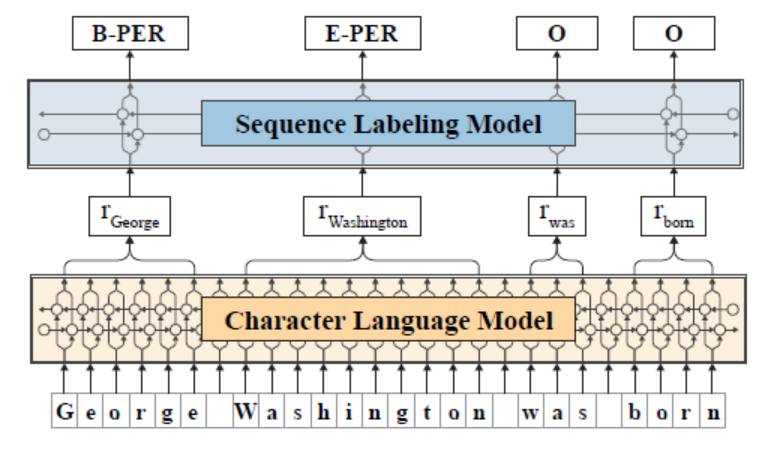
\includegraphics[scale=.5]{imagenes/2_theorical_framework/information_extraction/sequenceLabelingModel.PNG}
    \caption{Flair Sequence Labeling architecture~\cite{seqlab:flair-AkbikBBRSV19}}
    \label{fig:flairArchitecture}
\end{figure}		
	% Semantic Parsing
	\section{Semantic Parsing}
As mentioned by Kamath and Das~\cite{semPar:KamathD19}, Semantic Parsing is defined as the 
mapping from a natural language utterance into a semantic representation. These 
representations usually refer to logical forms, meaning representations or programs, which 
are executed over an underlying context such as relational tables or knowledge graphs. This 
execution yields a desired output like an answer to a question. For example, given a question 
in natural language, a semantic parser can aim to generate a valid SPARQL query based on the 
Wikidata’s ontology grammar that produces the correct answer when executed over a Wikidata 
endpoint.

The first component of a Semantic Parsing framework is the \textbf{language} to represent 
logical forms or meaning representations such as 
logic based formalisms~\cite{semPar:LiangBLFL16,semPar:ArtziFZ13}, 
graph based formalisms~\cite{semPar:BanarescuBCGGHK13,semPar:OepenKMZCFHU15} 
or programming languages~\cite{semPar:FeurerKESBH15}. In particular, we focus on query 
languages such as SQL or SPARQL. Another component is the \textbf{grammar}, which is a set of 
rules used to decide the expressivity of a semantic parser. Some examples are the Combinatory 
Categorial Grammar for complex structured queries~\cite{semPar:steedman1996}, or the Abstract 
Syntax Tree associated with a programming language’s defined grammar on general purpose code 
generation [ref]. A last component is the \textbf{underlying context}, which is the 
environment over which the output mappings are interpreted or executed. Knowledge Graphs such 
as Wikidata or DBpedia serve as examples of an underlying context.

The early attempts for Semantic Parsing were systems based on rules or statistical techniques. 
Among the rule-based systems, systems could be based on pattern matching~\cite{semPar:Johnson84a} 
or syntax-based systems~\cite{semPar:Woods73}. Though their implementation is simple, 
rule-based systems tend to be domain specific, thus hard to adapt to other domains. On the 
other hand, statistical models are able to train given examples of input-output pairs from 
any domain. Many approaches require a lexicon as a-priori 
knowledge~\cite{semPar:ZelleM96, semPar:ThompsonM03}, which is used to extract relevant 
semantic or syntactic information. Since these examples are usually manually annotated or 
require complex annotations, statistical models are hard to scale. There is also an issue 
with data sparsity, so these models only work in narrow domains.

Some of the most recent approaches that have emerged are based on Sequence-to-Sequence (Seq2seq) 
models, which usually uses an encoder-decoder framework based on neural networks. Some 
approaches implement an end-to-end paradigm where an intermediate representation is not 
needed to deliver a meaning representation; thus they do not rely on lexicons, templates or 
manually generated features. Though traditional approaches are able to better model and 
leverage the in-built knowledge of logic compositionality, approaches based on sequence 
models outperform traditional approaches due to the fact that Seq2seq-based models generalize 
better with more complex and longer sentences~\cite{semPar:JiaL16}. Furthermore, Seq2seq-based 
models can also generalize across domains~\cite{semPar:KamathD19}.

In the following subsections, we discuss in more depth how systems based on 
Sequence-to-Sequence models work. First, we will briefly explain Sequence-to-Sequence models 
along with the approach we will use in this work: the Convolutional Sequence-to-Sequence model. 
Then, we will introduce Neural Machine Translation systems and how these models can be used 
for the task of translating natural language questions to SPARQL queries.

\subsection{Sequence to Sequence models}

The Sequence-to-Sequence (Seq2seq) model was first introduced by 
Cho et al.~\cite{seqlab:ChoMBB14} [ref] for statistical Machine Translation. 
They proposed a neural network work model based on an encoder-decoder framework 
which is based on recurrent neural networks 
(RNNs)~\cite{semPar:werbos1990, semPar:rumelhart1986,seqlab:HochreiterS97}. More details 
about RNNs can be found in Appendix~\ref{appendix:neuralNetworks}.

In a Seq2seq architecture, the encoder converts a variable-length sequence into a fixed-length 
vector representation (i.e., it encodes the input sequence into a context vector) which is 
passed through to the decoder that transforms this fixed-length vector representation back 
into a variable-length sequence (i.e. decodes a context vector back to another output 
sequence). Figure~\ref{fig:seq2seqModel} illustrates graphically how a Seq2seq looks, where 
the length $T$ of the input sequence does not necessarily equal the length $T'$ of the output 
sequence.

\begin{figure}[!h]
    \centering
    
\includegraphics[scale=.5]{imagenes/insertImage.png}
    \caption{Sequence to Sequence model.}
    \label{fig:seq2seqModel}
\end{figure}

Technically, the model is learning a conditional distribution over a variable-length sequence 
conditioned on yet another variable-length sequence $p(y_1,\ldots,y_T'|x_1,\ldots,x_T)$. The 
encoder is an RNN that reads each symbol of an input sequence $x$ sequentially. While it is 
reading the current symbol on each step $t$, the hidden state $h_{<t>}^e$ of the RNN changes are
described as:

\[
    h_{<t>}^e= f(h_{<t-1>}^e,x_t)
\]

After reading the end of the sequence, the hidden state of the RNN is the summary $c$ of the 
whole input sequence, also known as its context vector. Then, the decoder is another RNN 
trained to generate the output sequence by predicting the next symbol $y_t$ given the hidden 
state $h_{<t>}^d$. This prediction is also conditioned on the previous predicted symbol 
$y_{t-1}$ and on the context vector $c$. Then, the hidden state of the decoder is defined 
for the step $t$, where $f$ is usually the \textit{sigmoid} function:

\[
    h_{<t>}^d= f(h_{<t-1>}^d,y_{t-1},c)
\]

Similarly, the conditional distribution of the next symbol, where $g$ is commonly a 
\textit{softmax} function since a valid probability must be produced, is defined as follows:

\[
    P(y_t|y_{t-1},y_{t-2},\ldots,y_1,c) = g(h_{<t-1>}^d,y_{t-1},c)
\]

Both components of the sequence model are jointly trained to maximize the following 
conditional log-likelihood function:

\[
    max_{\theta} \: \frac{1}{N} \sum_{n=1}^N log \; p(y_n|x_n)
\]

Once the model is trained, it can be used to generate a target sequence given an input 
sequence. Though Seq2seq models were originally designed based on RNNs, other variants have 
emerged~\cite{semPar:SutskeverVL14,nmt:DongL16}; among the more modern ones, a recent work 
introduces a sequence learning approach based on convolutional neural networks, which has 
shown to outperform many RNN-based models in the task of NL-to-SPARQL~\cite{nmt:nl-to-sparql-Yin19}.

\subsubsection{Convolutional Sequence to Sequence Model}
A Sequence-to-Sequence model based completely on convolutional neural networks (CNNs) is 
proposed by Gehring et al.~\cite{nmt:convS2S-GehringAGYD17}, called the Convolutional 
Sequence-to-Sequence model (ConvS2S). For this subsection we will assume a basic 
understanding of CNNs, where more details about this topic can be found on 
Appendix~\ref{appendix:neuralNetworks}.

Since CNNs do not receive the input as a sequence like RNNs do, a \textbf{position embedding} 
is proposed. First, the input elements $x=(x_1,\ldots,x_m)$ are embedded in distributional 
space as $w=(w_1,\ldots,w_m)$, where $w_j$ is a column in an embedding matrix $D$. These 
embeddings are combined with an absolute position vector $p=(p_1,\ldots, p_m)$, which 
indicates the position of the word in the sequence, in order to establish a sense of order in 
the input. From this combination the input element representation $e=(w_1+p_1,\ldots, w_m+p_m)$ 
is obtained. The output elements generated by the decoder are built using a similar 
representation.

To compute intermediate states, a simple convolutional block structure is used for both 
encoder and decoder, where such blocks are also referred to as layers. These intermediate 
states are based on a fixed number of input elements whose output for the l-th block are 
denoted as $z^l=(z_1^l,\ldots,z_m^l)$ for the encoder network and $h^l=(h_1^l,\ldots,h_m^l)$ 
for the decoder network. Each block contains a one dimensional convolution followed by a 
non-linearity.

Each convolution kernel is parameterized as $(W, b_w)$ and takes as input $X$, which is a 
concatenation of $k$ input elements embedded in $d$ dimensions, and maps them to a single 
output element $Y$. Subsequent blocks operate over the k output elements of the previous 
block. The gated linear unit (GLU)~\cite{semPar:DauphinFAG16} was chosen as the non-linearity 
to apply over the output of the convolution Y. This gating mechanism permit to control which 
input values of the current context are relevant. Aside from that, to enable deep convolutional 
networks, residual connections are added from the input of each convolution to the output of the 
block~\cite{semPar:HeZRS15}.

The input of the encoder network is padded to match the output length of the convolutional 
blocks for each block. The padding is done by adding $k - 1$ zero vectors on both the left 
and right side of the input to then remove k elements from the end of the convolution output. 
The same padding cannot be done for the decoder network since no future information is known 
beforehand~\cite{semPar:OordKK16}.

A linear mapping is added for projecting between the embedding size and the convolution 
outputs. This mapping is applied to $w$ when feeding embeddings to the encoder network, to the 
encoder output $z_j^u$, to the final block of the decoder just before the softmax $h^L$, and 
to all decoder blocks $h^l$ before computing the attention score, which is explained later. 

Lastly, a distribution is calculated over the $T$ possible next target elements $y_{i+1}$ by 
transforming the top decoder output $h_i^L$ via a linear layer with weights $W_o$ and bias 
$b_o$, as follows:

\[
    p(y_{i+1}|y_1,\ldots,y_i,x)=softmax(W_o h_i^L + b_o)
\]

Besides convolutional block structures, a separate \textbf{attention mechanism} is implemented 
for each decoder layer. Attention allows the model to focus on the relevant parts of the 
sentence for each time step. The entire process is illustrated in 
Figure~\ref{fig:convBlockStruct}. The calculation of the attention starts in the bottom left 
part of Figure~\ref{fig:convBlockStruct} with a combination between the current decoder state 
$h_i^l$ and the embedding of the previous target element $g_i$, which is defined as:

\[
    d_i^l= W_d^l h_i^l + b_d^l + g_i
\]

Then looking at the center part of Figure~\ref{fig:convBlockStruct}, for a decoder block $l$, 
the attention $a_{ij}^l$ of state $i$ and source element $j$ is computed as a dot-product 
between the decoder state summary $d_i^l$ and each output $z_j^u$ of the last encoder block $u$:

\[
    a_{ij}^l = \frac{exp(d_i^l \cdot z_j^u)}{\sum_{i=1}^m exp(d_i^l \cdot z_j^u)}
\]

Subsequently, the conditional input $c_i^l$ to the current decoder block is a weighted sum of 
the encoder outputs as well as the input element embeddings $e_j = w_j + p_j$ which corresponds 
to the center right part of Figure 1, and is defined as:

\[
    c_i^l = \sum_{j=1}^m a_{ij}^l (z_j^u + e_j)
\]

Finally, the conditional input $c_i^l$ is added to the output of the corresponding decoder layer 
$h_i^l$, as seen in the bottom right part of Figure~\ref{fig:convBlockStruct}. Compared with the 
classical single step attention, this proposal is named a multi-step attention mechanism since 
each step takes into account the attention history of the previous time steps, based on how 
conditional inputs are computed. Thus, information does not struggle to survive several steps 
as happens with recurrent networks.

\begin{figure}[!h]
    \centering
    
\includegraphics[scale=.5]{imagenes/insertImage.png}
    \caption{Convolutional block structure with a multi-step attention mechanism~\cite{nmt:convS2S-GehringAGYD17}}
    \label{fig:convBlockStruct}
\end{figure}

Some \textbf{normalization strategies} are applied to stabilize the learning process. First, 
the input and output of a residual block are summed with $\sqrt{0.5}$ to halve the variance of 
the sum. Second, the conditional input $c_i^l$ are scaled by $m\sqrt{1/m}$ to counteract any 
change in variance. Lastly, for convolutional decoders with multiple attention, the gradients 
for the encoder blocks were scaled by the number of attention mechanisms used, excluding source 
word embeddings.

Besides scaling, a \textbf{weight initialization} is also done to keep variance retained. 
Embeddings are initialized from a normal distribution with mean 0 and standard deviation 0.1. 
Weights from layers whose output is not directly fed to a GLU are initialized from 
$\mathcal{N}(0, \sqrt{1/n_l})$, where $n_l$ is the number of input connections to each neuron. 
This helps to maintain a variance of the input with a normalized distribution. Layers followed 
by a GLU are initialized from $\mathcal{N}(0, \sqrt{4/n_l})$, which is a weight initialization 
scheme based on works by He et al.~\cite{semPar:HeZRS15} and Glorot \& Bengio~\cite{semPar:GlorotB10}. 
Biases are uniformly set to zero. Lastly, dropout is applied to the input on some layers with a 
probability of p of being retained and so scaled by $1/p$, or setting them to zero 
otherwise~\cite{semPar:SutskeverVL14}.

\subsection{Natural Language to SPARQL}
Though most works have focused on translating text to SQL queries~\cite{nmt:CaiXZYLL18,nmt:ZhongCoRR17}, 
recent work has also addressed the translation of natural language to SPARQL. In particular, 
Neural Machine Translation (NMT), which involves Machine Translation systems based on Neural 
Networks, has been used to develop systems that translate questions to SPARQL queries. An 
evaluation of eight different NMT models was performed by Yin et al.~\cite{nmt:nl-to-sparql-Yin19}]. 
The NMT models included in this work were based on the aforementioned encoder-decoder Seq2seq 
architecture. Among these models, six of them are based on recurrent neural networks (RNN), 
while the remaining two are based on the ConvS2S model~\cite{nmt:convS2S-GehringAGYD17} and 
the Transformer model~\cite{semPar:VaswaniSPUJGKP17} respectively.

The systems based on RNNs include a baseline and many variants of the same LSTM architecture 
and different types of attention mechanisms. As a baseline, a Neural SPARQL Machine 
(NSpM)~\cite{nmt:nspm-SoruMMPVEN17, nmt:CoRRSoru18} is used, which consists of a 2-layer LSTM 
model with no attention mechanisms. Then, two variants of the NSpM are used with two different 
types of attention: global attention and local attention. Global attention uses the entire 
input sentence to calculate an attention vector, which complements the context vector output by 
the encoder~\cite{nlToSparql:BahdanauCB14}. On the other hand, local attention only uses a 
fixed size window around every word of the sequence to calculate a scoped attention vector per 
word~\cite{nlToSparql:LuongPM15}. Another model is based on a proposal from 
Luong et al.~\cite{nlToSparql:LuongPM15}, which consists of a 4-layers LSTM model with local 
attention. Lastly, the Google Machine Translation (GNMT) architecture~\cite{nlToSparql:WuSCLNMKCGMKSJL16} 
is included with two different variants: a 4-layer LSTM and a 8-layer LSTM, both with local 
attention. The only difference between Luong’s model and the GNMT is that the second model 
includes residual connections from the third layer and uses a bidirectional LSTM in the first 
layer of the encoder.

\subsubsection{Neural Machine Translation}

Though the architecture of each model varies, the encoding of SPARQL queries used in all 
approaches is the same as that proposed by Soru et al.~\cite{nmt:nspm-SoruMMPVEN17}. Their 
encoding suggests that URIs are abbreviated using their prefixes  followed by an underscore; 
brackets and dots are replaced by their verbal description, and SPARQL keywords are lower-cased. 
For example, a query over Wikidata is shown in Listing~\ref{lst:decodedWikidataSparqlExample}, 
when after an encoding conversion, it is converted to an encoded query as seen in 
Listing~\ref{lst:encodedWikidataSparqlExample}.

\begin{lstlisting}[captionpos=b, 
    caption=SPARQL query before encoding., 
    label=lst:decodedWikidataSparqlExample,
    basicstyle=\ttfamily,frame=single]
PREFIX wd: <http://wikidata.org/wiki/>
PREFIX wdt: <http://wikidata.org/prop/direct/>

SELECT ?sbj 
WHERE {
    ?sbj wdt:P19 wd:Q201007 .
    ?sbj wdt:P166 wd:Q37922 .
}
\end{lstlisting}

After training, the system will output an encoded form that can be transformed back to the 
original SPARQL representation. 

\begin{lstlisting}[captionpos=b, 
    caption=SPARQL query after encoding (note it excludes the PREFIX clauses)., 
    label=lst:encodedWikidataSparqlExample,
    basicstyle=\ttfamily,frame=single]
select var_sbj where brack_open var_sbj wdt_p19 
wd_q201007 sep_dot var_sbj wdt_p166 wd_q37922 
sep_dot brack_close
\end{lstlisting}

The evaluation metrics typically used to compare these systems are string-matching accuracy, 
BLEU score and perplexity. The string-matching accuracy is used to measure the amount of exact 
matches delivered by each system. The global accuracy is then the percentage of cases that are 
syntactically equal to the expected answer. This metric is particularly useful when measured 
over a dataset based on SPARQL templates, giving insights into whether or not the expected 
SPARQL form is being correctly generated.

The Bilingual Evaluation Understudy (BLEU) score is used to measure how similar two sentences 
are by using a geometric average of modified n-gram precision~\cite{nlToSparql:PapineniRWZ02}, 
which is represented by the following formula:

\[
    BLEU = BP \cdot exp(\sum_{n=1}^N w_n \; log \: p_n)    
\]

The modified precision $p_n$ for each candidate counts the number of times an n-gram occurs in a 
reference translation(s), takes the maximum count of each n-gram among the reference(s), and 
then clips the count of each n-gram in the candidate translation to the maximum count. To avoid 
short candidate translations getting higher scores than desired, a brevity penalty (BP) is 
applied which is set to 1 if the candidate length $c$ is larger than the maximal reference 
length $r$ or set to $exp(1-r/c)$ otherwise. The wn represents weights for each modified 
precision. By default $w_n=\frac{1}{N}$ and $N=4$. In this case, the BLEU score goes from 0 to 
100, where a score closer to 100 means the model is performing better. Note that BLEU does not 
account for word order. 

\textbf{Perplexity} is used to understand the model’s intrinsic behavior based on a cross 
entropy H(p,q) which is defined as follows:

\[
    H(p,q)= -\sum_x p(x) \; log \: q(x)
\]

where $p$ represents the target probability distribution and q is the estimated probability 
distribution. Their similarity is defined by all possible values $x$ in the distribution. In 
this case, $p$ is the one-hot encoding vector of the target vocabulary and q is deduced from 
the result of the output softmax layer. Then the perplexity is defined as the exponentiation 
of the cross entropy:
\[
    perplexity(p,q)=2^{H(p,q)}
\]

According to the experiments conducted by Ying et al.~\cite{nmt:nl-to-sparql-Yin19}, the model 
that performs best was the ConvS2S model. Although many datasets were used in their experiments, 
we are only interested in LC-QuAD~\cite{dataset:lcquad2-DubeyBA019} and 
DBNQA~\cite{dataset:dbnqa-hartmann-marx-soru-2018}, two datasets that represent opposite traits 
of a Question Answering Dataset: the LC-QuAD dataset contains few questions (5000) but with high 
complexity and high variance of its questions while the DBNQA dataset contains a huge volume of 
questions (nearly 900,000) but it lacks variety in its questions. We explain with more details 
what we understand by a “good dataset” in the \textit{Question Answering} section. The results 
of the three best models among the eight selected over the mentioned datasets are shown in 
Table~\ref{table:nmtYinResults}.

\begin{table}[h!]
    \centering
    \resizebox{\textwidth}{!}{%
    \begin{tabular}{|l|l|l|l|l|l|l|l|l|l|l|l|l|}
    \hline
    \multirow{2}{*}{} & \multicolumn{4}{c|}{Perplexity}                           & \multicolumn{4}{c|}{BLEU Score}                           & \multicolumn{4}{c|}{Accuracy}                             \\ \cline{2-13} 
                    & \multicolumn{2}{c|}{LC-QuAD} & \multicolumn{2}{c|}{DBNQA} & \multicolumn{2}{c|}{LC-QuAD} & \multicolumn{2}{c|}{DBNQA} & \multicolumn{2}{c|}{LC-QuAD} & \multicolumn{2}{c|}{DBNQA} \\ \hline
    Models            & Train         & Valid        & Train        & Valid       & Valid         & Test         & Valid        & Test        & Valid         & Test         & Valid        & Test        \\ \hline
    LSTM\_Luong       & 1.12          & 4.92         & 1.9          & 2.15        & 52.43         & 51.06        & 77.64        & 77.67       & 0             & 0            & 34           & 34          \\ \hline
    ConvS2S           & 1.14          & 3.25         & 1.12         & 1.25        & 61.89         & 59.54        & 96.05        & 96.07       & 8             & 8            & 85           & 85          \\ \hline
    Transformer       & 1.16          & 3.15         & 2.21         & 3.34        & 58.99         & 57.43        & 68.68        & 68.82       & 7             & 4            & 3            & 3           \\ \hline
    \end{tabular}%
    }
    \caption{Performance comparison of three models included in Yin et al.\cite{nmt:nl-to-sparql-Yin19}}
    \label{table:nmtYinResults}
\end{table}

Based on the perplexity results, there is a serious overfit for all models over the LC-QuAD 
dataset which Yin et al. attributes to the small size of the dataset and its complex questions. 
No evident overfit is spotted over DBNQA, and the ConvS2S shows better results which is 
reflected in the other results as well. The BLEU score results reflect that ConS2S again 
outperformed all other models and shows a correlation between perplexity and BLEU, especially 
when looking at DBQNA results. Finally, accuracy results clearly show that RNN based models and 
the Transformer do not perform positively in any case when compared to the ConvS2S model. 
However, the results over the LC-QuAD again shows there is still a challenge to handle more 
complex questions among all NMT models.

	
	% Question Answering over Knowledge Graphs
	\section{Question Answering over Knowledge Graphs}
\label{cap2:qakg}
Question Answering systems respond to the need to access information on the Web without 
detailed knowledge of Semantic Web technologies such as how data is structured (RDF) or how to 
access data (SPARQL). In particular, Question Answering systems (QAS) provide end-users with an 
intuitive and easy-to-use user interface, which hides the complexity behind the Semantic Web 
standards~\cite{qa:intro-UngerFC14}. These systems differ from traditional search engines such 
as Google in that search engines only return documents in which the answer can be potentially 
found, whereas a Question Answering system aims to return precise answers~\cite{qa:LopezUSM11}.

When we mention the task of Question Answering over Knowledge Graphs (QAKG), we refer to 
receiving a natural language question and returning an answer retrieved from one or more 
Knowledge Graphs (e.g. the first man to walk on the moon is Neil 
Amstrong\footnote{\url{https://www.wikidata.org/wiki/Q1615} in Wikidata}). Though there is work which 
includes a wider context along with the question, such as hybrid questions or chain of questions, 
we focus only on the problem of responding to an individual question without further context 
besides the question itself.

Another consideration for defining the scope of Question Answering is the question and answer 
type a system aims to respond to/with. Among the types of questions for which a Question 
Answering system usually provides an answer are:

\begin{itemize}
    \item \textbf{Definition question}, refers to a definition of a subject or object (e.g. 
    \textit{“Who was Violeta Parra?”}).
    \item \textbf{Factoid questions}, which are related to facts. This type of questions 
    includes three different variants:
    \begin{itemize}
        \item \textbf{Predicative questions} that refer to a specific object related to a predicate 
        such as who, what, where, how (e.g. \textit{“Who was the first man in space?”}, 
        \textit{“What is the highest mountain in Chile?”}).
        \item \textbf{List questions} that refer to all the answers that fulfill the fact being 
        asked (e.g. \textit{“Give me all the countries in America“}).
        \item \textbf{Boolean questions} that refer to whether the fact being questioned is true 
        or not (e.g. \textit{“Was Gabriela Mistral a poet?”}).
    \end{itemize}
\end{itemize}

In the context of Linked Data, a Question Answering system is limited to the information the 
available knowledge graphs can represent. For instance, questions not based on specific facts 
such as process questions (e.g. \textit{“How do I make a lemon pie?”}) or opinion questions 
(e.g. \textit{“What do most Chileans think of global warming?”}) cannot be answered.

Questions can also be classified depending on the answer type expected. One example is the work 
of Xin Li et al.~\cite{qa:LiR02}, which classify questions given five high-level categories: 
\textbf{entities} (e.g. event, color, animal, plant), \textbf{descriptions} (e.g. definition, 
manner, reason), \textbf{humans} (e.g. individual, group), locations (e.g. city, country, 
mountain) and numbers (e.g. count, date, distance, size). Another way is to classify questions 
according to its \textbf{focus} and \textbf{topic}, representing what the question is about. 
For instance, the question \textit{“What is the height of Aconcagua mountain?”} focuses on the 
property height in the topic of geography while the question \textit{“What is the best 
height-increasing drug?”} focuses on the same property, but a different topic, which is medicine.

According to Fu et al.~\cite{qa:FuQTLYS20abs-2007-13069}, current systems do not struggle with 
answering simple questions, i.e. questions that only require one subject-predicate-object 
triple fact, but complex questions are still a challenge for QAKG. A complex question usually 
is referred to as three types: questions under specific conditions (e.g. \textit{“Who was the 
president of Chile during the Great Recession of 2008?”}), questions with more intentions (e.g. 
\textit{“Give the names of the Chilean national football team and the number of goals they have 
scored”}), and questions requiring constraint inference (e.g. \textit{“What is the most 
expensive movie starring Pedro Pascal?”}).

\subsection{QAKG approaches}
\label{cap2:qakg/approaches}
Though there is no standard approach for QAKG, most techniques or methods proposed follow a 
similar four-stage pipeline~\cite{qa:core-techniques-DiefenbachLSM18}. First, a question 
analysis stage includes techniques that extract information from the current question using 
purely syntactic features. Then, the phrase mapping stage defines techniques that identify KG 
resources for each named entity and its dependencies. Next, the disambiguation stage 
encapsulates techniques that rank and determine for each named entity the most relevant 
resources according to the context of the question. Lastly, the query construction stage 
considers techniques used to construct the SPARQL query that should retrieve the final answer. 
In summary, most Question Answering systems are a combination of these four steps and vary with 
respect to which techniques are used to address each phase of the Question Answering process.

On the other hand, QAKG approaches can be classified according to which techniques their models 
are based on. The traditional QAKG models rely on predefined templates and manuals to parse 
questions [ref]. However, these traditional approaches require a certain level of knowledge of 
linguistics, and tend to be difficult to scale. Therefore, recent work has focused more on two 
kinds of approaches: methods based on Information Retrieval methods and other ones based on 
Neural Semantic Parsing.

\subsubsection{Information Retrieval-based methods}
\label{cap2:qakg/approaches/infRetrieval}
Information Retrieval (IR) based models reduce the QA task to binary classification or sorting 
over candidate answers. An IR-based method usually begins by identifying relevant entities 
mentioned in the question. Then, it extracts topic-entity-centric subgraphs where all nodes are 
considered candidate answers. Next, candidates are scored using features that provide semantic 
relevance and help to select the final answers. Depending on how the feature representations 
are built, IR-based methods can be divided into those based on feature engineering and those 
based on representation learning.

Methods based on feature engineering rely on manually defined and extracted features. For 
example, Yao et al.~\cite{qa:YaoD14} extract four types of features based on the question’s 
syntactic information, which includes question words, question focus words, topic words, and 
central verbs. These features are used in a classification model to determine the final answer. 
However, building these features is time-consuming and is not able to capture the entire 
semantic information of questions.

Methods based on representation learning convert questions and candidate answers into vector 
representations and reduce QAKG to a semantic matching computation between representations of 
questions and their candidate answers. Some methods incorporate external knowledge to complement 
the representation information and address the incompleteness that the KG might 
have~\cite{qa:XuRFHZ16,qa:SunDZMSC18,qa:TrouillonWRGB16}. Some other methods incorporate a 
multi-hop reasoning process to handle more complex questions~\cite{qa:SukhbaatarSWF15,qa:MillerFDKBW16,qa:QiuWJZ20}.

Overall, IR-based models get rid of manually defined templates and rules, and can follow an 
end-to-end training. However, these methods lack model interpretability and are not able to 
handle complex questions that require constraint inference.

\subsubsection{Neural Semantic Parsing-based methods}
\label{cap2:qakg/approaches/neuSemParsing}
In this context, methods based on Semantic Parsing aims to convert natural languages into 
executable query languages. Methods based on Neural Semantic Parsing (NSP) rely on Neural 
Networks to enhance the parsing capacity and scalability, instead of relying on predefined 
templates or rules. Thus, these models aim to map unstructured questions to intermediate 
logical forms which are later converted to structured queries.

One approach is to use query graphs, which are graphs that encoded questions, have strong 
representation ability and share topological commonalities with knowledge graphs. One example 
is GraphParser, proposed by Reddy et al.~\cite{qa:ReddyLS14} which frames the Semantic Parsing 
problem as a Graph Matching problem. Derived from GraphParser, the Staged Query Graph 
Generation~\cite{qa:YihCHG15} (STAGG) and the Multiple Constraint Query Graph~\cite{qa:BaoDYZZ16} 
(MultiCG) were proposed. While STAGG proposed a different construction of the query graph based 
on a restricted subset of lambda-calculus in the graph representation, MultiCG extends STAGG to 
include more constraint types and operators in order to cover more complex questions. Since all 
these proposals rely on Entity Linking tools to initialize the query graph construction, 
Yu et al.~\cite{qa:YuYHSXZ17} assumes a poor performance of such tools and proposes a 
Hierarchical Residual BiLSTM with the goal of improving entity recognition accuracy.

On the other hand, other work proposes to use encoder-decoder models to reduce the Semantic 
Parsing task into a Sequence-to-Sequence problem. One example is the Seq-to-Tree model proposed 
by Dong et al.~\cite{nmt:DongL16} that uses a hierarchical tree-structured decoder to capture 
the structure of logical forms. Then, in order to take more advantage of the syntactic 
information of the input question, the Graph-to-Seq model was proposed by Xu et al.~\cite{qa:XuWWYCS18} 
to encode the question as a syntactic graph. A last example is the Neural Symbolic Machine 
proposed by Liang et al.~\cite{qa:LiangBLFL17}, which proposed a lighter supervision approach 
by training a Seq-to-Seq model with reinforcement learning. Nevertheless, none of the examples 
mentioned above have been evaluated in the context of QAKG.

In general, the results of NSP-based models tend to be slightly better than the results from 
IR-based models. Nevertheless, it is still challenging to train a Neural Semantic Parser due to 
the lack of training data.

\subsection{Main Challenges}
\label{cap2:qakg/challenges}
The QAKG task is still an open problem, where many challenges have partially been addressed. 
Some of these challenges are related to the question being asked and others to the answers that 
can be returned. 

There are different ways to express the same question, as there are different ways to represent 
information within Knowledge Graphs. The \textbf{lexical} gap is the difference between the 
vocabulary used in a question and how information is expressed in the Knowledge 
Graph~\cite{semPar:lexical-gap-HakimovUWC15}. The bigger this gap is, the more difficult it is 
for QA systems to locate the correct resources for each named entity identified. 

Some work has tried to address the lexical gap, where most techniques are based on string 
normalization, pattern matching or entailment. For example, string normalization methods such 
as converting to lower case or stemming (e.g. convert \textit{“writing”} to its base form 
\textit{“write”}) help to reduce the search space when mapping entities. Another example are 
pattern libraries, such as PATTY~\cite{qa:NakasholeWS12} or BOA~\cite{qa:GerberN12}, that 
support pattern matching from a phrase to a resource. Nevertheless, most techniques proposed 
are based on manually defined rules, which is hard to scale or to transfer to other Knowledge 
Graphs.

Another challenge related with input expressivity is the \textbf{ambiguity} bound to each 
question, in other words, questions with different semantic meaning but with similar syntactic 
structure. There two main types of ambiguities: homonymy, when different concepts are 
represented by a string with the same spelling (e.g. the word \textit{“right”} can refer to 
\textit{“correct”} or \textit{“direction opposite to left”}), and polysemy, when one string can 
represent different but related concepts (e.g. \textit{“newspaper"} can refer to a 
\textit{”printed publication”} or to a \textit{”media company”}). 

Among the approaches used to address ambiguity are corpus-based methods or resource-based 
methods. Usually the corpus-based methods use statistical models from unstructured text 
corpora~\cite{qa:shirai1997,qa:ShenYYJLC11}. On the other hand, resource-based methods take 
advantage of the RDF properties of candidate resources. A score is calculated for each entity 
following the assumption that a better score applies a higher probability of a resource to be 
chosen. Some examples are RVT, which uses Hidden Markov Models~\cite{qa:GiannoneBB13}; CASIA, 
which relies on Markov Logic Networks~\cite{qa:shizhu2014casia}; or Treo~\cite{qa:freitas2011treo,
qa:FreitasOOSC13}, which uses Wikipedia-based semantic relatedness.

Unlike the lexical gap, which affects the recall of a QA system, ambiguity negatively affects 
its precision. While some methods aim to reduce the lexical gap, these same methods can make it 
difficult to address ambiguity. It is customary that in the disambiguation stage the systems 
try to balance the effects of both issues.

From challenges that are related to the query construction, the needs of \textbf{complex operators} 
affect the capability of a QA system to respond to more complex questions. The difficulty to 
handle a question increases when several facts have to be identified. Some examples that have 
tried to addresses these issue are YAGO-QA~\cite{qa:AdolphsTSUW11}, which tries to address 
nested questions; PYTHIA~\cite{qa:UngerC11}, which can answer question involving quantifiers, 
comparatives, superlatives and others; and IBM Watson~\cite{qa:GliozzoK12}, which can respond 
to indirect questions and multiple sentences.

As mentioned before, there are certain types of questions that current QA systems struggle to 
handle. One example is that of \textbf{procedural questions} (i.e. describe a procedure), which 
no QA system has been able to solve. Another example relates to \textbf{temporal questions} 
which refer to questions that require inferring temporal relation between events, though some 
works have tried to address temporal questions~\cite{qa:Allen83,qa:FerrandezSKDFNITONMG11,
qa:MeloRN11}. A last example relates to \textbf{spatial questions} that include questions 
referring to locations. The capability of answering spatial questions depends on how the schema 
of the knowledge represents locations (e.g. latitude and longitude), and how QA systems can use 
that information to enrich semantic data~\cite{qa:YounisJTA12,qa:graph-2-ZouHWYHZ14}.

The use of \textbf{templates} is thus more common to construct SPARQL queries that include 
complex operators such as aggregation or filter functions. These SPARQL query templates can be 
either manually or automatically created. One template-driven approach is Casia~\cite{qa:shizhu2014casia} 
that uses the question type, named entities and POS tagging techniques to generate graph 
pattern templates from which a SPARQL query is built. Other approaches use manually created 
templates combined with machine learning methods~\cite{qa:AbachaZ12}. 

\subsection{Benchmark \& Datasets}
\label{cap2:qakg/benchmarkDatasets}
In order to measure a Question Answering system performance, the most common parameters used 
across all benchmarks are \textbf{Precision}, \textbf{Recall} and \textbf{F1-score}. These 
three metrics usually are based on a gold standard set per question, which are the entities or 
values expected to be returned by the QA system. Given a question $q$, the formulas for Recall, 
Precision and F1-score are represented in the following formulas:

\begin{equation}
    \begin{aligned}
    Recall(q) &= \frac{\mbox{number of correct system answers for q}}{\mbox{number of gold standard answers for q}} \\
    Precision(q) &= \frac{\mbox{number of correct system answers for q}}{\mbox{number of system answers for q}} \\
    F1(q) &= \frac{2 \ast Precision(q) \cdot Recall(q)}{Precision(q)+Recall(q)}
    \end{aligned}
\end{equation}

As an example, given the question \textit{“Which are the primary colors?”}, the gold standard 
answer would be [\textit{“red”}, \textit{“green”}, \textit{“blue”}]. If a system answer is [
\textit{“brown”}, \textit{“green”}], the Precision would be 0.5 since \textit{“green”} is the 
only color part of the correct answers among the two colors returned, while the Recall would be 
0.33 because the only color correctly returned among the golden standard set is \textit{“green”}.

Similar to Entity Linking system evaluations, the global precision or global recall can be 
reported in two ways: as a micro average or a macro average. The F1-score is also used to 
combine  precision and recall into one measure.

In recent years, many datasets have been developed to include complex questions. In particular, 
we will briefly describe the datasets used in this work whose questions often require complex 
query construction and provide the expected query and result.

\subsubsection{QALD}
\label{cap2:qakg/benchmarkDatasets/qald}
The series of QALD datasets are part of the Question Answering over Linked Data (QALD) challenges, 
which aim to provide an up-to-date benchmark for measuring performance and comparing Question 
Answering systems~\cite{qa:qald-Lopezetal2013}. The QALD challenge is divided into multiple 
tasks that invite QA systems to address different challenges of Question Answering: 
multilinguality, hybrid questions, large-scale question answering and adaptability to other 
data sources. Though most versions of QALD contain questions that can be only answered over 
DBpedia, one of the versions of QALD did contain questions over Wikidata for the task of 
adaptability.

That being said, the $7^{th}$ version of QALD (QALD-7)~\cite{dataset:qald7-UsbeckNHKRN17} includes a 
dataset of 150 questions over Wikidata, divided into 100 questions for training and 50 for 
testing. The questions comes from a real-world question and query logs, where each question is 
manually annotated and includes a manually specified SPARQL query. Regarding the complexity of 
the questions, about 38\% are considered complex, including questions with counts, superlatives, 
comparatives, and temporal aggregations.

Despite the good quality of the questions of QALD-7 and its proximity to real-world questions, 
its limited size means that it is insufficient for training NSP-based models, which require a 
considerable amount of annotations to undergo a successful learning process

\subsubsection{LC-QuAD}
\label{cap2:qakg/benchmarkDatasets/lcquad}
The Large-Scale Complex Question Answering Dataset (LC-QuAD) is a dataset based on 
DBpedia~\cite{dataset:lcquad-TrivediMDL17}, where 82\% of its questions are considered complex. 
Differently from QALD, the SPARQL queries are built using a relatively small number of 
predefined templates, thus generating a large high-quality dataset with low domain-expert 
intervention. This results in a dataset that contains a total of 5000 questions with their 
corresponding queries.

Their dataset construction pipeline follows a different proposal to the standard one, where 
instead of writing the natural language question and then its logical form (aka the SPARQL 
query), the process is inverted. Thus the process starts by filling 38 hand-made SPARQL 
templates with seed entities and relations from a preferred predicate list to generate specific 
SPARQL queries. After that, a natural language question (NLQ) is deduced, for each generated 
SPARQL query, following a three-step process: a generation of a normalized NLQ by filling a 
Normalized Natural Question Template (NNQT) with the entity and relations names used to 
generate the current query, a verbalisation of the normalized NLQ using crowdsourcing tools, 
and a final validation done by an independent reviewer.

The proposal of LC-QuAD was a first step to allow NSP-based models to be applied to the field 
of Question Answering in the RDF/SPARQL setting, though most works~\cite{qa:FuQTLYS20abs-2007-13069} 
show that a larger amount of examples are still required to train models properly.

\subsubsection{DBNQA}
\label{cap2:qakg/benchmarkDatasets/dbnqa}
The DBpedia Neural Question Answering (DBNQA) [ref] dataset is thus far the largest dataset for 
Neural Question Answering over DBpedia, with 894,499 annotated pairs. The process to construct 
this dataset is similar to the one proposed for LC-QuAD, though its templates are extracted 
from the multilingual QALD-7 train dataset that includes 215 questions (not the same dataset as 
the Wikidata QALD-7 dataset mentioned before) and the same LC-QuAD dataset. This extraction 
process provides 5217 SPARQL templates. Another difference is the approach to generate natural 
language questions. This dataset originated from the purposes of training Neural SPARQL 
Machines, mentioned in the \textit{Semantic Parsing} section.

The template extraction process for each case consisted of replacing the concrete entities 
with placeholders. This is the case for the original question, where resource labels are 
replaced, and the query, where entities are replaced. This process functioned differently for 
the two datasets used. For the QALD-7-Train~\cite{dataset:qald7-UsbeckNHKRN17} dataset the 
resources were manually replaced, while for LC-QuAD an automatic script was implemented taking 
advantage of the fact that the resources were marked in the questions. As an example, given the 
question \textit{“What are the artists that are born in Stockholm?”} which generates the query 
in Listing~\ref{lst:dbnqaSparqlExample}, the template extraction process would return a 
question template \textit{“What are the artists that were born in <A>?”}, replacing the 
resource Stockholm, and would generate the query template shown in Listing~\ref{lst:dbnqaTemplateExample}.

\begin{lstlisting}[captionpos=b, 
    caption=SPARQL query for the question: \textit{"What are the artists that are born in Stockholm?"}., 
    label=lst:dbnqaSparqlExample,
    basicstyle=\ttfamily,frame=single]
SELECT DISTINCT ?sbj WHERE {
    ?sbj dbp:placeOfBirth dbr:Stockholm .
    ?sbj rdf:type dbo:MusicalArtist .
}
\end{lstlisting}

\begin{lstlisting}[captionpos=b, 
    caption=Query template for the question: \textit{"What are the artists that are born in <A>?"}., 
    label=lst:dbnqaTemplateExample,
    basicstyle=\ttfamily,frame=single]
SELECT DISTINCT ?sbj WHERE {
    ?sbj dbp:placeOfBirth <A> .
    ?sbj rdf:type dbo:MusicalArtist .
}
\end{lstlisting}

Then, the dataset is constructed following a similar approach to the one used for LC-QuAD. 
First, a set of entities is chosen per query template, where the entities selected are the ones 
that contain the relations contained in the query (e.g. if the property location is contained 
in the query, places would be selected accordingly). Then the selected entities are used to 
generate each SPARQL query with its corresponding NLQ. 

Since the construction of each case does not include a paraphrasing stage, there is almost no 
variation of questions that comes from the same template, i.e. there was no syntactic 
difference for questions with the same purpose. This lack of variation negatively affects the 
generalisation capabilities of NSP-based models trained on this dataset~\cite{qa:BerantL14}.

\subsubsection{LC-QuAD-2}
\label{cap2:qakg/benchmarkDatasets/lcquad2}
Taking into account all the advantages and disadvantages of the aforementioned datasets, a 
second version of the Large-Scale Complex Question Answering Dataset (LC-QuAD-2) was 
proposed~\cite{dataset:lcquad2-DubeyBA019}. In particular, this dataset provides around 30,000 
questions over Wikidata which contains complex questions and high diversity among its questions. 
The dataset generation workflow combines semi-automatic question generation along with a 
crowdsourced-based paraphrasing phase.

SPARQL queries are generated given a set of entities, predicates and templates) do not differ 
much compared to the first version of LC-QuAD. Nevertheless, the SPARQL templates used are 
different from the ones used before. Now the templates are based on one of the 10 types of 
question LC-QuAD-2 aims to address:

\begin{enumerate}
    \item \textbf{Single fact}: use a single (S-P-O) triple query, e.g. \textit{"Who is the 
    screenwriter of Mr. Bean?"}.
    \item \textbf{Single fact with type}: the fact is focused on the type of constraint, e.g. 
    \textit{"Billie Jean was on the tracklist of which studio album?"}.
    \item \textbf{Muti-fact}: use two connected facts, e.g. \textit{"What is the name of the 
    sister city tied to Kansas City, which is located in the county of Seville Province?"}.
    \item \textbf{Fact with qualifiers}: includes more informative facts stored in qualifier 
    properties, e.g. \textit{"What is the venue of Barack Obama’s marriage ?"}.
    \item \textbf{Two intentions}: consider questions with two intentions and also rely on 
    qualifiers, e.g. \textit{"When and where did Barack Obama get married to Michelle Obama?"}.
    \item \textbf{Boolean}: ask whether a fact is true or false, including questions with 
    number as an object, e.g. \textit{"Did Breaking Bad have 5 seasons?"}.
    \item \textbf{Count}: uses the COUNT keyword to perform a numeric count over a certain fact, 
    e.g. \textit{"What is the number of Siblings of Edward III of England ?"}.
    \item \textbf{Ranking}: requires counting and sorting in order to rank entities regarding a 
    certain property, e.g. \textit{"What is the binary star which has the highest color index?"}.
    \item \textbf{String Operation}: applies string operations at a work or character level, 
    e.g. \textit{"Give me all the Rock bands that start with the letter R?"}.
    \item \textbf{Temporal aspect}: covers temporal properties where various time facts are 
    included in qualifier properties, e.g. \textit{"With whom did Barack Obama get married in 1992?"}.
\end{enumerate}

Considering that some types of questions might have more than one SPARQL template variation, a 
total of 22 templates are used. 

\begin{figure}[!h]
    \centering
    
\includegraphics[scale=.45]{imagenes/insertImage.png}
    \caption{Example of LC-QuAD 2 question workflow generation.}
    \label{fig:lcquad2Pipeline}
\end{figure}

Then, a set of relevant entities and a predicate list is selected based on each SPARQL template, 
meaning that each question type includes different entities and properties (e.g. the property 
\textit{“birthPlace”} might not be used for questions that require counting). For each case, a 
subgraph is built based on three factors: an entity, the SPARQL template, and one or more 
suitable predicates. From each subgraph a SPARQL query is generated. Next, each SPARQL query is 
transformed to a normalized natural language question, called a Question Template (QT), which is 
then verbalised and paraphrased in a three-step pipeline based on human turkers from the Amazon 
Mechanical Turk tool (a crowdsourcing tool to perform simple tasks on a large scale). 

The first step is to convert each QT into Verbalised Question (QV), where most of the 
grammatical errors and semantic inconsistencies of the QT are fixed. The second step is to 
paraphrase each QV, where the resulting Paraphrased Question (QP) should preserve the overall 
semantic meaning while changing its syntactic content and structure. An example of the entire 
generation of one case is illustrated in Figure~\ref{fig:lcquad2Pipeline}. The last step is a 
human verification where a comparison is done between each QT with its corresponding QP in 
order to measure the quality of the final result in terms of semantic similarity.

After the entire generation process, a dataset is provided with around 52\% complex questions 
and significant variation in their  question structure. There is, however, a small percentage 
of error derived from using a crowdsourcing tool [ref], with questions losing part of their 
semantic intent or questions that are poorly verbalized/paraphrased, which should be taken into 
consideration when using this dataset to train NSP-based models. 
	
% Sistema propuesto
\chapter{System Overview}
\label{cap3:system}
In this chapter we describe the main components of the proposed Question Answering system. 
First we briefly provide a general overview of the proposed system structure, and then explain 
in more detail each of the modules implemented for this work.

\section{Question Answering general overview}
\label{cap3:system/qaPipeline}
The Question Answering pipeline is divided into different stages, as seen in 
Figure~\ref{fig:questionAnsweringOverview}, which do not differ much from the standard 
Question Answering pipeline described by Lopez et al.~\cite{qa:core-techniques-DiefenbachLSM18}. 
We assume that the target Knowledge Graph is Wikidata for the purposes of the example, but 
the architecture can be applied more generally to any Knowledge Graph. For the question 
\dquotesit{Was Gabriela Mistral a poet?}, the expected answer can be retrieved from the 
Wikidata query service by executing an ASK-type \SPARQL{} query. In other cases a SELECT query may be 
required.

\begin{figure}[!h]
    \centering
    \includegraphics[scale=.5]{imagenes/3_system_overview/QuestionAnsweringPipeline.png}
    \caption{Question Answering system pipeline.}
    \label{fig:questionAnsweringOverview}
\end{figure}

In order to build this \SPARQL{} query, the Question Answering system starts with 
a Query Template Generation stage to generate \SPARQL{} Query Template candidates with 
placeholders to be filled with entities in a later stage. These entities are first annotated 
in the Entity Linking stage, where relevant labels are identified (e.g., \dquotesit{Gabriel 
Mistral} or \dquotesit{poet}) and linked to their corresponding entity Knowledge Graph. 

The process of filling the annotated entities on the placeholders of a Query Template is not a 
straightforward process. In the example provided in Figure~\ref{fig:questionAnsweringOverview},
the entity of \dquotesit{Gabriel Mistral} (\texttt{Q80871}) should be the subject 
of a triple in a \SPARQL query, but in other contexts this entity could be the object of a triple. 
Sometimes Entity Linking may recognize more entities than placeholders to be filled, 
thus adding another layer of complexity that an Entity Linking system cannot exclusively address.
Therefore, the Slot Filling stage aims to identify which entities should be used to 
fill which placeholders of the Query Template candidates. 

The Question Answering pipeline described in the Figure~\ref{fig:questionAnsweringOverview} 
is implemented by building three modules that execute each one of the described stages. 

\section{Query Generation Module}
\label{cap3:system/queryGenModule}
In this section we describe the Query Generation Module, which is used by the Baseline system 
and adapted for the system proposed in this work. Given a Natural Language (NL) question, the 
goal is to generate its logical form in terms of \SPARQL{} grammar, which can be either a 
complete \SPARQL{} query representation (baseline) or an intermediate Query Template 
representation (our system).

We now explain the main components that encapsulate the Query Generation module. First, we 
describe the Query Generation pipeline, which does not differ much between the generation of 
an entire \SPARQL{} query or its Query Template. Then, we explain the Query Encoding used to 
deliver a normalized expression of the expected output for the model that performs the 
generation process. Finally, we describe in more detail how the model is trained and used to 
generate queries based on the FairSeq library for implementing Sequence to Sequence models in 
Python.

\subsection{Query Generation pipeline}
\label{cap3:system/queryGenModule/pipeline}
This module addresses two different tasks: translation from NL to \SPARQL{} queries, and 
generation of Query Templates from NL. 

On one hand, when we refer to \SPARQL{} queries, we refer to complete queries with all the 
entities, properties, \SPARQL{} keywords and operators necessary to be executable on any 
Wikidata endpoint. Previous works on this task are usually based on Sequence-to-Sequence 
models, where many have SQL as their target language~\cite{nmt:DongL16, nmt:CaiXZYLL18, 
nmt:ZhongCoRR17}. Most recent works apply similar models targeting \SPARQL{}~\cite{nmt:CoRRLuz18, 
nmt:nspm-SoruMMPVEN17, nmt:CoRRSoru18}.

On the other hand, Query Templates refer to intermediate representations of \SPARQL{} queries, 
which instead of containing the necessary entities included in a complete \SPARQL{} query, 
contain placeholders that will be later filled using the entities obtained in the Entity 
Linking stage. An example of both cases can be found in Figure~\ref{fig:queryGenerationOverview}, 
where the left side shows a \SPARQL{} query, and the right side its Query Template. 

\begin{figure}[!h]
    \centering
    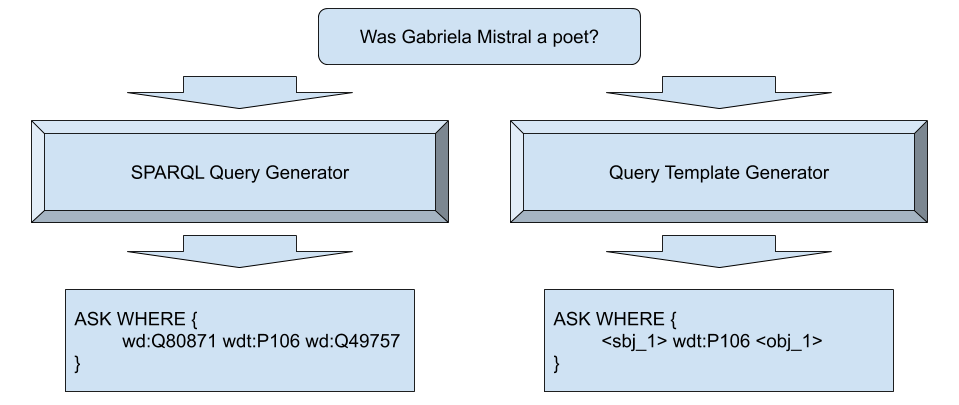
\includegraphics[scale=.5]{imagenes/3_system_overview/queryGenerationPipeline.png}
    \caption{Query Generation pipeline example.}
    \label{fig:queryGenerationOverview}
\end{figure}

In Figure~\ref{fig:queryGenerationOverview}, we can see the Query Generation pipeline and 
expected output for both tasks given the input NL question \dquotesit{Was Gabriela Mistral a 
poet?}. On the left, the \SPARQL{} query pipeline outputs an ASK-type \SPARQL{} question with two 
entities involved. On the other side, a Query Template is returned, which looks like an 
ASK-type \SPARQL{} query but it replaces the entities for two placeholders indicating that there 
is a subject entity and an object entity expected in the first triple of the Query Clause. 
The idea of the Query Template is that these placeholders will later be filled by the Slot 
Filling module.

As we mentioned before, the Query Generation pipeline does not change whether the model is 
generating an entire \SPARQL{} query or just an intermediate Query Template, and there are two 
reasons that explain this. First, both tasks can be seen as translating NL to a meaning 
representation, where such representations only vary on the information they are displaying. 
While generating a \SPARQL{} query includes the entities involved in the query, the generation 
of a Query Template replaces those entities for placeholders indicating that in those places 
an entity or a plain value will be needed, without specifying which ones. The second reason 
is that both models rely on the same data: a set of pairs of NL questions and \SPARQL{} queries. 
The only difference is that the output data used for the Query Template model is adapted to 
fit the Query Template generation task, where entities and plain values (e.g. numbers or 
strings values) are replaced by a placeholder that keeps a certain degree of information for 
the replaced value (e.g. placeholder type, query triple position, etc). This dataset 
adaptation process is explained in more detail in the \textit{Experimental Design} chapter~\ref{cap4:experimentalDesign}.

Aside from the input and output process, there are some intermediate steps performed over the 
input and output data. In the case of the input NL questions, a normalization process is 
conducted where the question string is lower-cased and non-relevant symbols are removed. On 
the output side, an encoding process is performed over the data used for training, and a 
decoding process is done for the query string output by the Query Generator system. The Query 
Encoding is done by tokenizing the \SPARQL{} grammar, allowing to treat it as a target wordy 
language, following the idea of reducing this problem to a Machine Translation task used in 
previous works~\cite{semPar:ChoMGBBSB14, semPar:sempar-as-mt-AndreasVC13, nmt:nl-to-sparql-Yin19}. 
Then, each of the two Generator models shown in Figure~\ref{fig:queryGenerationOverview} 
corresponds to a previously trained Fairseq model, which receives a normalized NL question 
and returns an encoded meaning representation that has to be later decoded to obtain the 
final \SPARQL{} query or Query Template output.

\subsection{Query Encoding}
\label{cap3:system/queryGenModule/encoding}
Following the same encoding approach used by Soru et al.~\cite{nmt:nspm-SoruMMPVEN17}, we 
encode the \SPARQL{} queries into tokens that describe entities, keywords, symbols, and 
operations. One difference is that we are using a dataset that includes new query components 
such as numbers or string values; thus we propose novel tokens to encode those values. An 
example of this encoding can be seen in Listing~\ref{lst:encodingSPARQLSoru}. The main advantage of 
this encoding is that it allows the system to express chunks of commonly used patterns (e.g. 
order by asc/desc, or filter patterns) in a simpler way, thus reducing the complexity of the 
translation task.

\begin{sparqlcode}[%
    caption={\SPARQL{} query example with its encoded form.}, 
    label={lst:encodingSPARQLSoru}]
ASK WHERE { wd:Q658 wdt:P1108 ?obj FILTER(?obj < 1.2) }

ask where brack_open wd_q658 wdt_p1108 var_obj filter attr_open var_obj math_lt 1_dot_2 attr_close brack_close
\end{sparqlcode}

Query Templates are encoded in a similar way, but instead of encoding entities, numbers or 
string values, placeholders are used to replace those values. Besides those components, there 
is no other difference in the encoding process. Listing~\ref{lst:encodingTemplateSoru} shows 
the Query Template of Listing~\ref{lst:encodingSPARQLSoru} and its encoded form.

\begin{sparqlcode}[%
    caption={\SPARQL{} query example with its encoded form.}, 
    label={lst:encodingTemplateSoru}]
ASK WHERE { <sbj_1> wdt:P1108 ?obj FILTER(?obj < <num>) }

ask where brack_open placeholder_sbj_1 wdt_p1108 var_obj filter attr_open var_obj math_lt placeholder_num attr_close brack_close
\end{sparqlcode}

Note that instead of using letters for naming each placeholder as done by Ying et al.~\cite{nmt:nl-to-sparql-Yin19} 
(e.g. \texttt{A}, \texttt{B} or \texttt{C}) we use labels that provide more information about 
placeholders. For example, we identify placeholder type (subject, object, string value or 
numeric value) and position for entities placeholder (e.g. \texttt{sbj\_1} corresponds to the 
subject of the first triple in the Query clause).

These placeholder labels are also used in the Slot Filling system mentioned later in order to 
identify which entities output by the Entity Linking system corresponds to each one of the 
Query Template placeholders. 

\subsection{Fairseq Model}
\label{cap3:system/queryGenModule/fairseqModel}
The Query Generation model is implemented using the \textit{Facebook AI Research Sequence-to-Sequence 
Toolkit} (Fairseq), which implements various Seq2seq models based on Pytorch. Fairseq 
provides various off-the-shelf implementations and other settings to configure user 
experiments. 

In particular, we use the Convolutional Sequence to Sequence model (ConvS2S)~\cite{nmt:convS2S-GehringAGYD17} 
implementation to build the Query Generator model. The decision to use the ConvS2S is based 
on the work done by Yin et al.~\cite{nmt:nl-to-sparql-Yin19}, where eight Sequence-to-Sequence 
models were implemented and compared regarding the NL-to-SQL task. From this comparison, 
the ConvS2S model ended up having the best performance in terms of Perplexity, BLEU score, 
and string-match Accuracy. This model has to be trained and can be used later to generate an 
output depending on the given data. If we need to build a \SPARQL{} Query generator, we have to 
feed the system with pairs of NL questions and \SPARQL{} queries. In the same way, for a Query 
Template generator we instead use Query Templates as our output examples for training.

We now explain the main components of the ConvS2S architecture, the hyperparameters used with 
their values, and other training settings relevant to comprehend the training process. Note 
that the architecture used and its configuration is done following the work from 
Yin et al.~\cite{nmt:nl-to-sparql-Yin19}.

The ConvS2S architecture components used are based on the best-performance settings for 
natural language NMT~\cite{nmt:nl-to-sparql-Yin19}. In particular, the most relevant 
hyperparameters are the followings:

\begin{itemize}
    \item The number of \textbf{layers} used for the convolutional encoder and decoder is 15. 
    From these layers, the first 9 layers use $3 \times 3$ kernels with 512 units, the next 4 layers 
    use $3 \times 3$ kernels with 1024 units, and the final 2 layers uses a $1 \times 1$ kernel with 2028 units.
    \item The \textbf{optimizer}, i.e. the learning algorithm used, is Stochastic Gradient 
    Descent with minibatches. The default minibatch size is 64.
    \item The \textbf{learning rate} is set to fixed value of 0.5, which is maintained during 
    the entire training session.
    \item As a regularizer, \textbf{dropout} is applied with a fixed value of 0.2.
\end{itemize}

Besides those parameters, the Multi-step Attention mechanism is applied to some layers. The 
loss function used is the cross-entropy function mentioned in the \textit{Theoretical 
Framework} chapter~\ref{cap2:theoFrame/semPar/seq2seq}.

The training process is performed using Google Colaboratory, an online research tool that 
allows for writing and executing Python code and provides free computational resources, such 
as GPUs, to boost the training process. It is mainly focused on developing machine learning 
tasks. We also follow the same dataset split used by Yin et al.~\cite{nmt:nl-to-sparql-Yin19}: 
80\% for training and 20\% for dev/test. One difference is we only use train and dev sets, 
since other datasets are proposed as test sets. We chose this strategy as some of the 
existing datasets we use contain related or paraphrased questions, where creating an 
independent test set ensures that test questions are not derived from, or variants of, 
training questions. Each model is trained for a maximum amount of 40 epochs, where after 
every epoch a checkpoint is saved. Then, the checkpoint that achieves the lowest loss value 
for the validation set is kept.

The best values obtained from the training process can be imported later to the same Fairseq 
model implementation to perform new evaluations. When decoding on the evaluation stage, beam 
search is applied with a beam width of 5. As a last note, the same normalization process done 
for the training data has to be done with every new NL question. On the other hand, to obtain 
the \SPARQL{} query or the Query template it is always necessary to perform the decoded process 
over the Query Generator output.

\section{Entity Linking Module}
\label{cap3:system/entLinModule}
Two types of Entity Linking systems are considered for this work: Individual Entity Linking 
systems and Ensemble Entity Linking systems. First we discuss the pipeline that these systems 
follow.

\subsection{Entity Linking pipeline}
\label{cap3:system/entLinModule/pipeline}
An example for the Entity Linking pipeline is shown in Figure~\ref{fig:entityLinkingPipeline}, 
for the question \dquotesit{Was Gabriela Mistral a poet?}. We assume that the Entity Linking 
module is available through an API; the Entity Linking system first retrieves the annotations 
by querying the API service, which returns annotations along with extra information (e.g. scores, 
second ranking entities, etc). In the case that the Entity Linking system targets a different 
Knowledge Graph to the one over which questions are answered, in a second (optional) phase the 
entities are mapped from the former to the latter (we do not compute the mapping in this work 
but rather assume that a mapping is made available).

\begin{figure}[!h]
    \centering
    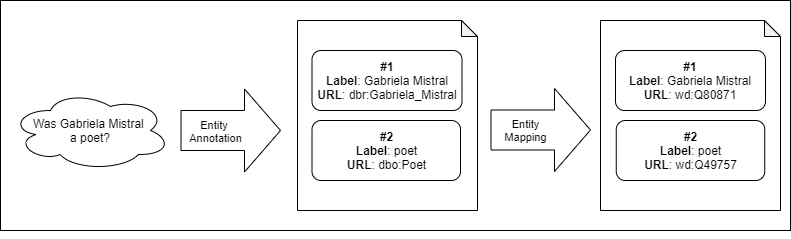
\includegraphics[scale=.5]{imagenes/3_system_overview/individualEntityLinkingPipeline.png}
    \caption{Entity Linking pipeline example.}
    \label{fig:entityLinkingPipeline}
\end{figure}

In this example, we show for each spotted mention: the start and end position, the annotation 
label and its associated resource. Then, an entity mapping process is performed to convert 
the DBpedia resources (\texttt{dbr:Gabriela\_Mistral} and \texttt{dbo:Poet}) into Wikidata 
resources (\texttt{Q80871} and \texttt{Q49757} respectively). As we mentioned, this 
mapping is optional and it depends on the target Knowledge Graph we are interested in, which 
in this case is Wikidata, and whether the system returns entities on that target Knowledge 
Graph.

The API service input parameters and output format is different for each web service, though 
the final output annotations from the Entity Linking module is always the same. An additional 
piece of information that is also returned are the scores each system gives to each annotation. 
Though these scores cannot be compared across systems, such scores are used to establish 
which entities are more relevant for each system. 

The Entity Mapping process assumes an existing mapping between the entities of both Knowledge 
Graphs. In this particular case, we can take advantage of the fact that many DBpedia resources 
and Wikidata resources are both bound to Wikipedia articles via the \texttt{schema:about} property. 
This information can be found on Wikidata, thereby, given a set of DBpedia entities, a \SPARQL{} 
query can be performed to retrieve their corresponding Wikipedia article and their related 
Wikidata entities, if any. An example of a \SPARQL{} query to map DBpedia entities to Wikidata 
ones can be seen in Listing~\ref{lst:entityMappingExample}.

\begin{sparqlcode}[%
    caption={\SPARQL{} query example to map DBpedia resources to Wikidata ones.}, 
    label={lst:entityMappingExample}]
SELECT ?article ?wikidata ?dbpedia WHERE {
    ?article schema:about ?wikidata .
    BIND(IRI(CONCAT("https://en.wikipedia.org/wiki/", SUBSTR(STR(?dbpedia),29))) AS ?article)
    VALUES ?dbpedia { <http://dbpedia.org/resource/Gabriela_Mistral> <http://dbpedia.org/ontology/Poet> }
}
\end{sparqlcode}

Following the same logic, Wikipedia articles can be mapped to their associated Wikidata resources. 
The opposite mapping from Wikidata resources to DBpedia ones can be easily performed as well. 
If any entity cannot be mapped from the results of the Entity Linking system to the target 
Knowledge Graph, it is discarded.

A final note about the entity mapping process is that it is performed over batches of entities, 
which means that a set of entities are mapped at the same time. This batch entity mapping is 
used to minimize the amount of queries done to the Wikidata query service. The final output 
values are returned in a JSON format.

\subsection{Individual Entity Linking systems}
\label{cap3:system/entLinModule/individualSystems}
We consider an Individual Entity Linking system as one of the Entity Linking systems mentioned 
in the Information Extraction chapter~\ref{cap2:theoFrame/infExtr/entityLinking}: 
DBpedia Spotlight~\cite{EL:dbpedia-spotlight-MendesJGB11}, 
AIDA~\cite{EL:aida-tool-YosefHBSW11, EL:aida-HoffartYBFPSTTW11}, TAGME~\cite{EL:tagme-FerraginaS10}, 
and OpenTapioca~\cite{EL:opentapioca-Delpeuch19}. These systems were selected because they 
provide public APIs that can be invoked over the Web. The annotation process is reduced to 
making a request on the corresponding API’s web service. We will briefly describe some details 
of the implementation and mention some aspects to take into consideration for each one of the 
aforementioned systems.

The \textbf{DBpedia Spotlight} system~\cite{EL:dbpedia-spotlight-MendesJGB11} aims to 
annotate DBpedia entities, so it requires a mapping process to convert the output annotations 
into Wikidata entities. The input parameters for the API request are the query text, a 
confidence value, and a support value. The confidence parameter is a threshold for disambiguation, 
and the support parameter is used to filter resources with a small number of Wikipedia 
inlinks. On the output side, DBpedia Spotlight assigns two scores to each entity: a 
similarity score, which represents how similar are the mention and the entity, and a 
percentage of second rank, which is the ratio of similarity scores between the second and the 
first candidates of the corresponding mention (used to measure the level of ambiguity for the 
mention).

The \textbf{AIDA} system~\cite{EL:aida-tool-YosefHBSW11, EL:aida-HoffartYBFPSTTW11} works over 
YAGO entities, though all YAGO entities map to a Wikipedia article. The annotations of this 
system can thereby be expressed as Wikipedia resources without the need for an extra query to 
the Wikidata query service. Nevertheless, the mapping process is done to map Wikipedia resources 
to Wikidata ones. Besides the text input parameter, the AIDA system does not require any other 
parameter. Each output annotation includes a disambiguation score which is the score assigned 
in the candidate ranking stage.

The \textbf{TAGME} system~\cite{EL:tagme-FerraginaS10} makes annotations over Wikipedia. As 
per AIDA, it requires a mapping stage to convert Wikipedia resources into Wikidata ones. 
Aside from the query text input parameter, TAGME requires a token parameter for authentication, 
which can be retrieved from its API website. Each entity annotation has a \dquotesit{rho} score 
assigned, which is derived from the candidate ranking stage.

The \textbf{OpenTapioca} system~\cite{EL:opentapioca-Delpeuch19} is the only one that works 
directly over Wikidata. It does not require any extra parameter besides the query text. In 
the output annotation, a logarithmic likelihood score is assigned to each annotation, which 
points out how prominent the entity is in the Wikidata Knowledge Graph.

As a general aspect, the GET requests of most of the systems’ web services are done using the 
\texttt{request}\footnote{\url{https://pypi.org/project/requests/}} Python library, except for AIDA 
where \texttt{curl}\footnote{\url{https://curl.haxx.se/}} requests are done using the subprocess 
Python library. Then, the mapping queries performed on the Wikidata query service are done 
using the \texttt{SPARQLWrapper}\footnote{\url{https://pypi.org/project/SPARQLWrapper/}} Python 
library.

\subsection{Ensemble Entity Linking system}
\label{cap3:system/entLinModule/ensembleSystems}
Besides each individual Entity Linking system, we propose an ensemble of Entity Linking systems 
in order to improve the performance in terms of recognizing all the entities in a given 
question. Since each individual system relies on different techniques or prioritizes different 
features, they can identify entities that are either very prominent or quite rare. In the 
context of Question Answering, if an Entity Linking system cannot identify all of the entities 
needed to build the required \SPARQL{} query, the Question Answering system will fail to provide 
the right answer. The inability to identify all entities is more prone to happen when little 
context is provided in the given text, which is a common situation in Question Answering 
settings.

An ensemble Entity Linking system aims to make the most of all individual Entity Linking 
systems by combining their results together to achieve better Recall and Precision. Then, an 
ensemble system is given the annotations of each individual system as the system input and 
returns a final output annotation set. We present two variants to combine the individual 
annotations: Precision Priority system and Voting system. To better illustrate the variants 
proposed in this work, let us assume that each individual 
Entity Linking system returns the following annotations, for the question \dquotesit{Does FC 
Barcelona have Juan Jose Ibarretxe as a chairperson?}:

\newpage

\noindent \textbf{AIDA}\\
\mbox{}\\
\begin{sparqlcode}[]
FC Barcelona - wd:Q7156
\end{sparqlcode}

\noindent \textbf{OpenTapioca}\\
\mbox{}\\
\begin{sparqlcode}[]
Juan Jose Ibarretxe - wd:Q351738  
\end{sparqlcode}

\noindent \textbf{TAGME}\\
\mbox{}\\
\begin{sparqlcode}[]
Juan Jose Ibarretxe - wd:Q351738    
chairperson - wd:Q140686  
\end{sparqlcode}

\noindent \textbf{DBpedia Spotlight}\\
\mbox{}\\
\begin{sparqlcode}[]
Does - wd:Q302057
FC Barcelona - wd:Q7156
Juan Jose Ibarretxe - wd:Q351738
chairperson - wd:Q140686    
\end{sparqlcode}

After the description of each variant, an example of the expected output annotations is given 
based on the results shown above.

In this example, the annotations expected to be recognized are the entities from \dquotesit{FC 
Barcelona} and \dquotesit{Juan Jose Ibarretxe}. Even though some systems recognized 
\dquotesit{chairperson} as an entity, the property \dquotesit{chairperson} (\texttt{wdt:P488}) 
is more likely to be used when building the \SPARQL{} query for this question, so its entity is 
not expected to be identified. Though this ambiguity issue (whether something is a property or 
an entity) can complicate building the \SPARQL{} query, it is not something that we address in 
the Entity Linking stage. Returning more entities than the number expected is still acceptable 
as long as the correct entities are included among the output annotations. However, we will 
see in the \textit{Slot Filling module} section~\ref{cap3:system/slotFillModule} that the more 
entities are passed from the Entity Linking stage, the more difficult it can be to find the 
correct entity-placeholder mapping. Thus, a threshold can be set to define the number of 
expected entities, which is commonly the number of slots contained in the predicted Query 
Template.

\subsubsection{Precision Priority system}
\label{cap3:system/entLinModule/ensembleSystems/pprior}
The Precision Priority (PPrior) ensemble system establishes that some individual Entity 
Linking systems are more likely to return the expected answers, which in this case are the 
individual systems that tend to return fewer entities but with a high level of confidence, 
i.e. systems that prioritize Precision over Recall.

Then, the PPrior system assigns a priority to each individual system according to their 
performance on the datasets we are interested in (\LCQuADtwo, \DBNQA, and \QALDseven). In 
particular, systems with better Precision have higher priority. These results can be found in 
the \textit{Results} chapter~\ref{cap5:results/entityLinking}, 
which establishes the following priority: AIDA, OpenTapioca, TAGME, and DBpedia Spotlight. Next, 
the PPrior system retrieves the annotations of each individual system following the established 
priorities until the number of unique expected entities is reached. 
For example shown above, the PPrior system would rank each entity in the following way:

\begin{sparqlcode}[]
1. FC Barcelona - wd:Q7156
2. Juan Jose Ibarretxe - wd:Q351738
3. chairperson - wd:Q140686
4. Does - wd:Q302057     
\end{sparqlcode}

The first entity (\texttt{Q7156}) comes from the AIDA system, the second one (\texttt{Q351738}) 
from OpenTapioca, the third one (\texttt{Q140686}) from one of the annotations output by 
TAGME (since the other entity has already been considered), and the remaining one (\texttt{Q302057}) 
comes from DBpedia Spotlight. Therefore, if the number of expected entities is two, the 
entities of the mentions \dquotesit{FC Barcelona} and \dquotesit{Juan Jose Ibarretxe} would be 
output as final annotations.

One advantage of this variant is that it would perform more efficiently in an online setting 
since it only requires to request annotations from the individual systems until it fulfills 
its expected number of entities. A disadvantage to take into consideration is that the PPrior 
system relies on the idea that systems with higher priority make fewer mistakes (e.g. 
recognize fewer false positives); thus incorrect entities from higher priority systems would 
have more value than correct entities from smaller priority systems.

\subsubsection{Voting system}
\label{cap3:system/entLinModule/ensembleSystems/voting}
The Voting ensemble system establishes a voting scheme where annotations from each individual 
system are considered to be a vote that is used to rank entities. This is based on the idea 
that if an entity is widely recognized across Entity Linking systems, that entity is more 
likely to be a correct annotation. Note that votes go for the entity identifier and not for 
the mention. Therefore, if two individual systems recognize the same entity but differ on the 
mentions linked, both systems are voting for the recognized entity (e.g. the \texttt{Q351738} 
entity could have been assigned to \dquotesit{FC Barcelona} or only to \dquotesit{Barcelona}, 
but votes go to the \texttt{Q351738} entity).

Given that ties are possible, the entities that come from more precise systems would have priority 
(following the same reasoning as with the PPrior system). For example, the Voting system 
would rank each entity in the following way:

\begin{sparqlcode}[]
1. (3) Juan Jose Ibarretxe - wd:Q351738
2. (2) FC Barcelona - wd:Q7156
3. (2) chairperson - wd:Q140686
4. (1) Does - wd:Q302057
\end{sparqlcode}

The most voted entity is \texttt{Q351738} with three votes, which comes from OpenTapioca, TAGME, 
and DBpedia Spotlight. Next, the entities \texttt{Q7156} and \texttt{Q140686} get the same 
amount of two votes. Since \texttt{Q7156} comes from a system with higher priority (AIDA), that 
entity ranks higher. The last entity \texttt{Q302057} only has one vote from the system with 
least priority (DBpedia Spotlight). Thereafter, if the number of expected entities is two, the 
entities of the mentions \dquotesit{Juan Jose Ibarretxe} and \dquotesit{FC Barcelona} would be 
output as final annotations.

The main advantage of the Voting system is that it can benefit from every system equally (all 
votes weigh the same regardless of their system’s Precision). Thus, it seems reasonable to 
assume that the more systems are included in the voting process, the greater the chances are 
that the correct entities will be among the top voted ones. Some disadvantages are that with 
few systems the voting system does not differ much from the PPrior system, and its process is 
more expensive to execute since it always requires retrieving the annotations from all 
individual systems included.

\subsubsection{Other optimizations}
\label{cap3:system/entLinModule/ensembleSystems/optimizations}
In order to improve the performance of Ensemble Entity Linking systems, a couple of heuristic 
optimizations are proposed to achieve better performance. These improvements are included in 
the two variants mentioned before, and are optional features that can be skipped if no 
significant improvement is perceived. 

First, some entities linked to stopwords (e.g. \dquotesit{Does} linked to \texttt{Q302057}) are 
filtered using an English stopwords list provided by the Natural Language Toolkit\footnote{\url{https://www.nltk.org/}}. 
Before performing any join annotation process, the annotations that contain stop words are 
discarded. The idea behind this filter is to avoid entities from systems with low Precision 
negatively affecting the identification of correct entities. However, some entities may 
include stopwords in their names (e.g. the rock band \dquotesit{The Who}), where this approach 
may negatively affect the results for such entities.

Lastly, a tiebreak system is implemented for entities that are ranked in the same position 
and come from the same system. Since each individual system assigns a score to each annotation, 
such scores can be used to break the tie and decide which entities will be considered in the 
final output. For example, if only two entities are expected but the second and third are 
tied (e.g. in the Voting system let us assume the entities from \dquotesit{Juan Jose Ibarretxe} 
and \dquotesit{chairperson} comes from OpenTapioca and have two votes each), we look at which 
has a higher score according to the individual Entity Linking system these annotations come from 
(i.e. which one has a higher \texttt{log\_likelihood} score according to OpenTapioca). 

\section{Slot Filling Module}
\label{cap3:system/slotFillModule}
In this section we describe the main components of the Slot Filling module, which is divided 
into two stages: the sequence labelling stage done by a Sequence Tagger, and the Query 
Filling stage where the spotted entities are filled into the given Query Template. We explain 
with details how the Slot Filling pipeline is structured, and then describe how the Sequence 
Tagger and the Query Filling algorithm are implemented.

\subsection{Slot Filling pipeline}
\label{cap3:system/slotFillModule/pipeline}
In Figure~\ref{fig:slotFillingPipeline}, we can see an overview of the Slot Filling process. 
Differently from the other modules, the Slot Filling system not only receives the input NL 
question, but also the outputs from the Entity Linking system and the Query Template generator. 
The expected output is a \SPARQL{} query which is based on the Query Template output by the 
Query Template generator, containing entities from the annotations returned by the Entity 
Linking system.

\begin{figure}[!h]
    \centering
    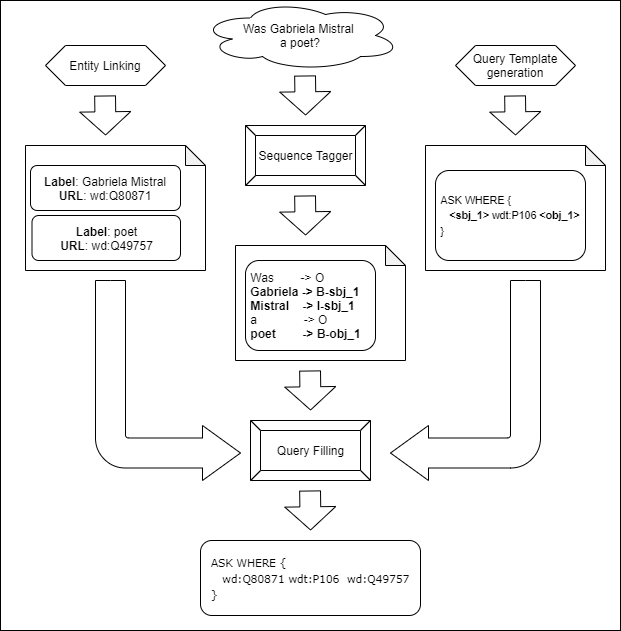
\includegraphics[scale=.5]{imagenes/3_system_overview/slotFillingPipeline.png}
    \caption{Slot Filling pipeline example.}
    \label{fig:slotFillingPipeline}
\end{figure}

Before the actual Slot Filling process, the input NL question is passed to a Sequence Tagger 
that identifies relevant named entities (or labels) and their 
corresponding placeholder tag. We understand a placeholder tag as a placeholder name in a 
Query Template. As seen in Figure~\ref{fig:slotFillingPipeline}, given the question 
\dquotesit{Was Gabriela Mistral a poet?}, the expected output for the Sequence Tagger is to 
identify \dquotesit{Gabriela Mistral} and \dquotesit{poet} as two relevant labels which 
are expected to have a Wikidata entity recognized by the Entity Linking system. For example, 
\dquotesit{Gabriela Mistral} is tagged as \dquotestt{sbj\_1}, meaning that the entity which 
corresponds to that label (\texttt{Q80871}) should be assigned to the placeholder 
\texttt{<sbj\_1>} in the Query Template. The same happened with the label \dquotesit{poet}, 
which should be assigned to the placeholder \texttt{<obj\_1>}. Note here that the goal is to 
infer label--placeholder annotations, whereas the Entity Linking system aims to produce 
label--entity annotations. 

Next, the labels tagged with their corresponding placeholder are passed to the Query Filling 
stage, along with the Entity Linking annotations and the generated Query Template. A filling 
algorithm is proposed to perform the Query Filling process. The algorithm will return a 
\SPARQL{} query only if the filling process is successful. As we will explain later, this filling 
process could fail due to the previous systems failing to recognize some entities, or due to 
a mismatch between the placeholders recognized in the tagging stage and the placeholder 
contained in the given Query Template.

\subsection{Sequence Tagger model}
\label{cap3:system/slotFillModule/seqTagger}
The Sequence Tagger identifies which labels are more likely to have an entity 
assigned to a certain placeholder in the Query Template. To implement this model, we use the 
Flair\footnote{\url{https://github.com/flairNLP}} framework for Natural Language Processing. Flair 
contains many off-the-shelf Sequence Labelling and Name Entity Recognition models implemented 
using Pytorch. It also supports  training a custom Sequence Labelling model if training data 
is provided.

We then adapt the same dataset used for generating the Query Template dataset to describe the 
expected output (more details in the \textit{Experimental design} chapter~\ref{cap4:experimentalDesign/datasets}). 
A Sequence Tagger model receives an NL 
question, and returns a sequence of tags where each tag is related to one word (or token) in 
the input question. These tags follow the BIO format, where each word is classified as the 
beginning of a tag, as the intermediate part of it, or as a non-tag token. For example, if 
given the question \dquotesit{Was Gabriela Mistral a poet?}, the expected output would be 
\texttt{(O, B-sbj\_1, I-sbj\_1, O, B-obj\_1)}. From this output we can infer that 
\dquotesit{Gabriela Mistral} is identified as one tag (\dquotesit{Gabriela} is the beginning of 
the tag and \dquotesit{Mistral} is an intermediate part of it), and \dquotesit{poet} is 
identified as another tag. On the other hand, the words \dquotesit{Was} and \dquotesit{a} are identified 
as non-tag tokens. Note that the length of the tagger output and the number of tokens in the 
input question are always the same amount, so every token is assigned with a BIO tag.

In this work three \textbf{types of placeholders} are chosen for three types of values: entities, 
numbers, and string values. The entity placeholder identifies entities from the Knowledge Graph 
resource (e.g. \texttt{Q80871}). Each entity placeholder identifies two aspects of the entity: 
1) its role in the query triple (subject or object), and its query triple position. For example, if 
an entity is tagged as \dquotestt{sbj\_1}, it means it is the subject of the first query triple. As 
their names may suggest, the number placeholder identifies numeric values, whereas the string value 
placeholder marks text relevant to the query (e.g. for filtering entities that contain a certain 
string label).

There are two main steps before training the Sequence Tagger model: preprocessing the 
dataset, and configuring the model architecture. The Sequence Labelling dataset has to be 
converted to a tag dictionary that fits the Flair model input. Each output value has to be 
expressed as a sequence of BIO tags. Whatever BIO tags are chosen determines the tags 
the Sequence Tagger will use. Next, the configuration of the model architecture is divided 
into embeddings and model settings. First, the embedding layer is set, where one or more 
types of embeddings can be joined into stacked embeddings. In this case, we use the GloVe 
embeddings along with contextual embeddings, also known as Flair embeddings~\cite{seqlab:flair-AkbikBBRSV19}. 
Lastly, the model architecture used is the same standard architecture used by 
Akbik et al.~\cite{seqlab:contextual-emb-AkbikBV18}, which is a BiLSTM~\cite{seqlab:HuangXY15} 
with the number of hidden layers set to 256, along with a CRF layer put on top of the final 
layer. 

Finally, there are some training parameters and settings that are defined by default and 
others that can be tuned for a particular task. Some default aspects include the learning 
algorithm (mini-batch stochastic gradient descent) and the loss function (cross-entropy 
function). Some relevant training parameters that can be tuned are the learning rate, the 
minibatch size, and the number of epochs. The model is trained until it has a fixed number of 
epochs without an improvement in terms of loss value.

\subsection{Slot Filling method}
\label{cap3:system/slotFillModule/fillingMethod}
The placeholder tags for each named entity, along with the annotations from the Entity 
Linking system and the Query Template from the Query Template generator, need to be combined 
together to build the final \SPARQL{} query output. The Slot Filling method decides which 
placeholder to replace with which entity, and is based on a novel filling algorithm divided 
into two filling stages. The first stage is a \textbf{Standard Filling} process that may not 
fill all the placeholders in the query, and the second stage is a \textbf{Force Filling} 
process that tries to complete the spots that the previous stage was not able to fill.

The first stage, the Standard Filling process, follows a straightforward process of comparing 
labels from the outputs of the Entity Linking system and the Sequence Tagger to identify 
entity-slot matches which are then inserted into the Query Template to form the \SPARQL{} query. 
Then, the algorithm that describes the standard filling process is shown in 
Listing~\ref{lst:standardFillingAlgorithm}. As an example from the input shown in 
Figure~\ref{fig:slotFillingPipeline}, the algorithm would first compare the label 
\dquotesit{Gabriela Mistral} with all the labels from the entity annotations. Then, it would 
be found that the placeholder \texttt{sbj\_1} should correspond to the entity 
\texttt{wd:Q80871} given that both labels are equal. Based on this match, the entity 
\texttt{wd:Q80871} should replace all the appearances of the placeholder \texttt{sbj\_1} in 
the current \SPARQL{} query that is being constructed.

\begin{sparqlcode}[%
    caption={Standard Filling algorithm.}, 
    label={lst:standardFillingAlgorithm}]
standard_filling(annotations, slots, query_template)
    sparql_query = query_template
    for s_label, placeholder in slots
        if placeholder has been used or placeholder not in sparql_query
            skip
        if placeholder is a <num> or <str_value>
            replace placeholder in sparql_query for the s_label value
        if placeholder is an <entity_type> (e.g. <sbj_1>)
            for e_label, entity in annotations
                if s_label equal to e_label
                    replace placeholder in sparql_query for the entity value
                    break
        mark placeholder and/or entity as used, if applies
    return sparql_query
\end{sparqlcode}

Some problems can arise from this algorithm, which are mainly due to previous systems passing 
incorrect or incomplete information (e.g. not all the entity annotations are identified, or 
the Sequence Tagger tag some mentions incorrectly). Consequently, some placeholders may not 
be filled by the standard filling process. In such cases, a second filling process, called 
Force Filling, is performed to address these issues.

Force Filling aims to fill all slots in a best-effort manner, and is performed based on some 
assumptions and heuristics. The first assumption is that since we usually deal with short 
questions, the number of entities to be identified and placeholders to be filled tend to be 
low, not having more than three spots to fill in average. We also assume that most of the 
mistakes made by the Sequence Tagger are due to incorrect tagging. Also, multiple word labels 
from annotations and from the Sequence Tagger might differ but if they share one or more 
words, it is more likely that both labels refer to the same value. Lastly, we assume that if 
one spot is left to be filled, and one entity is left to be used, it is likely that that 
entity should be placed there even if the slot label and the entity label are not the same. 
Considering all that, the mistakes made by previous systems can be mitigated by using simple 
heuristic rules. 

To summarize, a similar filling process to the one shown in Listing~\ref{lst:standardFillingAlgorithm} 
is executed, but adding the following rules:
\begin{itemize}
    \item If any slot label is contained in an entity label (or vice versa), it counts as a 
    match.
    \item When comparing entity type placeholders, if the slot placeholder is the same entity 
    type (subject or object) or is assigned to the same query triple (e.g. the first query 
    triple pattern on the \SPARQL{} query) as some of the remaining Query Template placeholders, 
    it counts as a match.
    \item Finally, if there is any remaining entity that was not identified by the Sequence 
    Tagger, and there are still placeholders to fill in the Query Template, the entities will 
    be inserted in order until all spots have been filled (where the order is defined by the 
    entity identifier number).
\end{itemize}

As an example, let us assume we have the outputs illustrated in Figure~\ref{fig:forceFillingExample} 
for the question \dquotesit{How many Nobel Prizes has Gabriela Mistral won?}, which requires a 
count operation. The expected slots state that the subject of the first query triple should 
be filled with the entity of the label \dquotesit{Gabriela Mistral}, while the object of the 
second query triple should be filled with the entity of the label \dquotesit{Nobel Prizes}. 
However, it may happen that a label is incorrectly associated with the wrong query triple 
(case 1), or the wrong entity type (case 2). In the first case, the \dquotesit{Nobel Prizes} 
entity would not be filled in the Standard Slot Filling stage due to the \texttt{<obj\_2>} 
not existing in the Query Template, but it would be recognized in the Force Slot Filling 
stage because it will identify that the remaining slot in the Query Template (\texttt{<obj\_1>}) 
is the same entity type as the slot incorrectly labeled (\texttt{<obj\_2>}). The same happens 
in the second case, where the incorrect label (\texttt{<obj\_1>}) is associated with the same 
query triple (the first triple) as the remaining slot in the Query Template (\texttt{<sbj\_1>}).

\begin{figure}[!h]
    \centering
    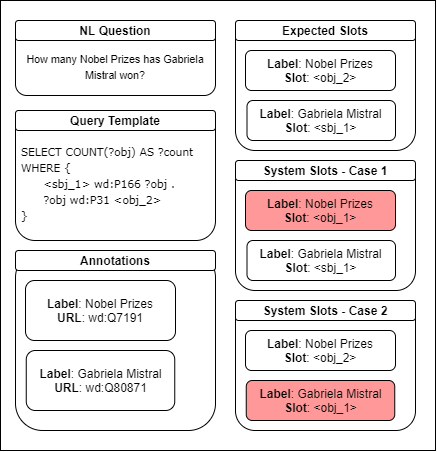
\includegraphics[scale=.5]{imagenes/3_system_overview/SlotFillingSpecialCases.png}
    \caption{Force Filling case examples.}
    \label{fig:forceFillingExample}
\end{figure}

Although more cases can be correctly filled by applying these rules, there are some other 
cases that are not possible to correctly fill. For example, the Sequence Tagger can identify 
the expected placeholder but it can wrongly associate each one to an incorrect mention (e.g. 
wrongly associate the subject entity and object entity of one query triple). A more serious 
case is when the Sequence tagger provides placeholders that have nothing to do with the ones 
found in the Query Template, usually because both systems identified a different intention in 
the given answer. In summary, the success rate of the filling process is strongly affected by 
the performance of the previous systems that deliver the input for this Slot Filling system.

% Disenho experimental
\chapter{Experimental Design}
\label{cap4:experimentalDesign}
We present an overview of the research questions we address in this work along with 
the details of the experimental design. The implementation of the system, experiments, and 
datasets used can be found in the following Github repository: \url{https://github.com/thesemanticwebhero/ElNeuKGQA/}.

\section{Question Answering general overview}
\label{cap4:experimentalDesign/QaOverview}
The task of Question Answering over Knowledge Graphs is far from being resolved, where one of 
the main challenges that still remains is answering complex questions. Current approaches rely 
mostly on hand-crafted rules, achieving decent performance over simple questions (that only 
require a few query triple patterns), but not for more complex questions. Complex questions are 
difficult to handle mainly because they may be structured in a more elaborate way, and most of 
them require the use of more advanced \SPARQL{} operations (such as aggregations, ranking, or the 
use of more complex graph patterns).

Some recent approaches based on Neural Networks have shown some potential for handling more 
complex questions. These Neural-based approaches usually aim to build the entire \SPARQL{} query 
given a natural question, reducing the problem of Question Answering to Semantic Parsing. The 
main weakness of these systems is that they are dependent on the vocabulary of the data used 
for training such models, so even though these systems can generalize to different question 
forms, they are not able to identify unknown entities that were not included in the training set.

In order to address this problem, we study the effectiveness of an approach that combines Neural 
Semantic Parsing with Entity Linking through a Slot Filling method proposed in this work. The 
research questions we propose are the following:

\begin{itemize}
    \item \textit{Can Entity Linking and Slot Filling improve the performance of Question 
    Answering systems over Knowledge Graphs based on Neural Semantic Parsing?}
    \item \textit{Which stages of the proposed Question Answering pipeline (Entity Linking, 
    Query Template Generation, Slot Filling) produce the most errors, what types of errors do 
    they produce, and how do they affect the overall performance of the Question Answering system?}
\end{itemize}

Note that all these questions are addressed specifically in the context of Wikidata as 
the target Knowledge Graph and for questions in English.

\section{Question Answering Dataset}
\label{cap4:experimentalDesign/QaDataset}
In this section we describe the dataset used for this work which includes the preprocessing 
required to improve the quality of the data used for training, validation and testing all of 
the modules (Query Generation, Entity Linking, and Slot Filling) and the final end-to-end 
Question Answering System. 

First, we describe the revision and cleaning performed over the \LCQuADtwo{} dataset, which is the 
main source we use to train the Neural Network-based models. Second, we explain the \SPARQL{} query 
encoding used for the training of the Query Template generation and the baseline \SPARQL{} Query 
Generation models. Third, we describe the process for generating the Query Templates used for 
training the Query Template generation model. Fourth, we describe the same process for the Slot 
Filling dataset. Finally, we present the normalized dataset format which we designed to handle 
all the datasets used.

\subsection{LC-QuAD 2 Dataset Cleaning}
\label{cap4:experimentalDesign/QaDataset/cleaning}
The \LCQuADtwo{} dataset requires a cleaning process where some cases were discarded or fixed due 
to various issues in either their question or \SPARQL{} query answer. First we mention which cases 
were discarded according to some problems found in their paraphrased or verbalized question. 
Next, we describe which cases were discarded according to problems found in their \SPARQL{} query. 
Since there are some queries with an easy fix, we explain briefly those cases. 

Given that the questions contained in the \LCQuADtwo{} dataset were built from a two-step 
question correction (a verbalization and a later paraphrasing), each dataset case contains 
three representations of the same question: a normalized question, a verbalized question and a 
paraphrased question. An example is shown in Listing~\ref{lst:questionExampleLcquad2}. Since 
this process was performed using a crowdsourcing tool, we found issues related with question 
verbalization (e.g., the human that performed the verbalization didn’t understand the normalized 
question) or loss of the question’s semantics through the conversion from normalized to 
paraphrased questions.

\begin{sparqlcode}[%
    caption={Example of questions contained in one case of the \LCQuADtwo{} dataset.}, 
    label={lst:questionExampleLcquad2}]
normalized question  -> Did {Alexander_Hamilton} {occupation} {lawyer}?
verbalized question  -> Is Alexander Hamilton a lawyer?
paraphrased question -> Did Alexander Hamilton practice law?
\end{sparqlcode}

A case is discarded if both the verbalized and the paraphrased questions present an issue. To 
define if a question is an invalid verbalization/paraphrase, the following issues are taken 
into account:

\begin{enumerate}
    \item The question is null, empty or not applicable (marked as \dquotestt{NA}). 
    \item The question has not been corrected, e.g., it still contains brackets from the normalized 
    question, or it is the same question as the normalized version without brackets.
    \item The question contains the answer to the previous normalized or verbalized question 
    instead of the verbalization or paraphrasing, respectively. 
    \item The length of the actual version compared with the previous version is too long or too 
    short, which for us is a way to identify the third issue or an indicator of a question that 
    did not maintain the semantic meaning of its previous version.
    \item The question is either too short or too long. We set a minimum of 4 tokens and a 
    maximum of 30, where each token is divided by whitespace characters.
\end{enumerate}

Note that given the large number of questions in the dataset, this validation was not performed 
manually but rather using a script to identify these issues as best as possible. Thus some 
undesirable cases may slip into the final preprocessed dataset, though we consider that as an 
acceptable amount of noise.

Other cases presented issues with their Wikidata \SPARQL{} query, where either the query was 
empty/null, or contained invalid entities or tokens. An entity is considered invalid if it does 
not present the common Wikidata pattern: a valid prefix (e.g. wd, wdt, etc) along with a valid 
identifier, which always is composed by a \texttt{Q} and a number (e.g. \texttt{Q80871}). A few 
queries contained invalid numbers such as \dquotestt{t1231} which are corrected by removing the 
\textit{t}. Some other queries presented syntax errors or had some clauses missing, which were 
corrected. Finally, a simple canonicalization process was performed over the variable names in 
order to follow similar conventions (e.g. use \texttt{sbj} and \texttt{obj} as base variable 
names).

Aside from that, some cases were duplicated due to the observation that they contained the same 
normalized question or the same \SPARQL{} query. Those with the same normalized question but 
different \SPARQL{} queries were merged into one case, though just one \SPARQL{} query is used later. 
Other cases with the same \SPARQL{} query (regardless of whether their normalized question is the 
same or not) were discarded.

% TODO: add explanation of complex cases
In summary, from the 30,226 cases contained in the \LCQuADtwo{} dataset, 2,520 cases were 
discarded: of these, 2,478 cases were discarded for having an invalid question or query, and 42 
cases were duplicate cases. Note that 52\% of this final preprocessed dataset is composed of 
complex questions (a deeper explanation of which cases are considered complex can be found in 
Appendix~\ref{appendix:qaDataset}). After preprocessing, this dataset is used to train the 
Neural-based models used in this work.

\subsection{Query Template Dataset}
\label{cap4:experimentalDesign/QaDataset/queryTemplate}
From the cleaned \LCQuADtwo{} dataset, a Query Template dataset was created for training the 
Query Template generator model. More specifically, a Query Template was inferred from each 
\SPARQL{} query by replacing every subject and object entity in the query with a placeholder. 
As explained in the System Overview chapter~\ref{cap3:system/slotFillModule/seqTagger}, in order 
to maintain some degree of the semantic meaning of the entity that is being replaced, we 
propose using several types of placeholder labels. For example, an entity that was the subject 
of the first query triple will be replaced by a placeholder labeled as \dquotestt{sbj\_1}. For 
numerical or string values, the placeholder would be \dquotestt{num} or \dquotestt{str\_value}, 
respectively. This is a different approach to generate Query Templates than the one followed by 
Yin et al.~\cite{nmt:nl-to-sparql-Yin19}, where instead they replaced entities by one-letter 
names such as \texttt{A}, \texttt{B} or \texttt{C}.

\begin{sparqlcode}[%
    caption={\SPARQL{} query and its Query Template version.}, 
    label={lst:queryTemplateExampleLcquad2}]
# SPARQL Query
SELECT ?obj WHERE { wd:Q14752155 wdt:P19 ?obj }

# Query Template
SELECT ?obj WHERE { <sbj_1> wdt:P19 ?obj }
\end{sparqlcode}

An example can be seen in Listing~\ref{lst:queryTemplateExampleLcquad2}, where in the \SPARQL{} 
query for the question \dquotesit{Where was Pedro Pascal born?} the entity \texttt{Q14752155} 
from Pedro Pascal was replaced for the \texttt{sbj\_1} placeholder. All queries from the cleaned dataset 
were able to be transformed into their Query Template version.

Since some cases may have issues with either the verbalized or the paraphrased question, we 
decided to maintain a one-to-one correspondence between question and query. Although it would 
be interesting to test whether having many variations of the same question might affect the 
system performance, we think such an experiment has to be done with a dataset where each case has 
the same amount of variations (which cannot be guaranteed with this dataset without having to 
discard an uncertain amount of valid cases). Then, in each case we first use the paraphrased 
question as the case’s question. However, if the paraphrased question is not valid, we use the 
verbalized question instead (if it is valid).

\subsection{Sequence Labeling Dataset}
\label{cap4:experimentalDesign/QaDataset/seqLabeling}
In order to train the Sequence Labeling model from the Slot Filling module, a dataset was 
needed. As per the Query Template dataset, the Slot Labeling dataset is based on the cleaned 
\LCQuADtwo{} dataset. The creation of this dataset is divided into two stages. 

The first stage consists of identifying the entity-label mapping in terms of which part of the 
question corresponds to each entity from the ones contained in the \SPARQL{} query. In the example 
of \dquotesit{Where was Pedro Pascal born?}, the label \dquotesit{Pedro Pascal} contained in the 
question should correspond to the entity \texttt{Q14752155} corresponding to the Chilean actor Pedro 
Pascal. This mapping identification was performed using the Wikidata labels found in the normalized 
question provided in the \LCQuADtwo{} dataset (see an example in Listing~\ref{lst:questionExampleLcquad2}).

In the second stage, the labels identified previously are associated with the placeholders used 
for the creation of the Query Template. In this case, the placeholder \texttt{sbj\_1} shown in 
Listing~\ref{lst:sequenceLabelingExampleLcquad2} corresponds to the entity \texttt{Q14752155}, 
therefore the label \dquotesit{Pedro Pascal} will be associated with the placeholder \texttt{sbj\_1}. 
We use the BIO label format as the output format for the Sequence Tagger, as shown in 
Listing~\ref{lst:sequenceLabelingExampleLcquad2} (the \squotestt{?} is ignored).

\begin{sparqlcode}[%
    caption={BIO label representation for a Natural Language Question.}, 
    label={lst:sequenceLabelingExampleLcquad2}]
# NL Question
Where was Pedro Pascal born ?

# Expected label output
O O B-sbj_1 B-sbj_1 O
\end{sparqlcode}

Some labels were not able to be associated with their corresponding placeholders due to the 
question rephrasing performed over the \LCQuADtwo{} dataset. The main issue was the discrepancy 
between the Wikidata label associated with an entity, and its current label in the question 
(which may be modified due to the rephrasing). As opposed to what we did for the Query Template 
dataset, we decided to add both verbalized and paraphrased valid cases to compensate 
for the loss of information. After processing the dataset, we ended up with 36,854 valid cases 
from the 52,853 initial cases (counting for each case its verbalized and paraphrased version), 
which is almost 70\% of the dataset.

\subsection{Final Dataset Format}
\label{cap4:experimentalDesign/QaDataset/finalFormat}
After extracting the Query Templates, the entities, and their entity/placeholder slots, a final 
\LCQuADtwo{} dataset was built containing all this information. In summary, each case possesses a 
question identifier, the question string, a Wikidata \SPARQL{} query, their entities with the 
corresponding label, a Query Template deduced from the \SPARQL{} query, and a mapping between the 
entity labels and the Query Template placeholders. 

We proposed a normalized format and delivered a dataset that not only can be used to evaluate 
systems on the KGQA task, but also over the tasks of Entity Linking, Name Entity Recognition, 
Slot Filling, Intent Classification, or Semantic Parsing. A sample of the entire dataset can be 
found in Appendix~\ref{appendix:qaDataset}.

\section{System Implementation}
\label{cap4:experimentalDesign/systemImplementation}
The system implementation was divided into three main modules which represent each stage 
described in the \textit{System Overview} chapter~\ref{cap3:system}: Query Generation, Entity Linking, and Slot 
Filling. These modules were assembled in our proposed Question Answering system, which receives 
a Natural Language question as an input, and returns a Wikidata \SPARQL{} query that can be executed 
on the Wikidata service endpoint as an output. The Question Answering system only returns a valid 
\SPARQL{} query; otherwise, if one cannot be computed, it will return nothing. The entire system was implemented 
using Python 3.6. 

The implementation of the two variants on the Query Generation module (SPARQL Query Generator 
and Query Template Generator) was divided into two stages. First the models were trained on 
Google Colaboratory\footnote{\url{https://colab.research.google.com/}} using the 
ConvS2s~\cite{nmt:convS2S-GehringAGYD17} model implementation included in the Fairseq 
framework\footnote{\url{https://fairseq.readthedocs.io/en/latest/}} and the settings described in the 
Fairseq Model subsection in the \textit{System Overview} chapter~\ref{cap3:system/queryGenModule/fairseqModel} 
(we recall that this model had 
the best performance in the comparison of Yin et al.~\cite{nmt:nl-to-sparql-Yin19}). After the 
training phase, a Fairseq Wrapper was implemented in order to import the models and perform the 
prediction over new data. These wrappers receive the NL question as the input and can return 
either the best predicted sequence, or a list with the best $N$ predictions (where $N$ can be a 
number defined by the user).

The various individual Entity Linking systems (DBpedia Spotlight~\cite{EL:dbpedia-spotlight-MendesJGB11}, 
AIDA~\cite{EL:aida-tool-YosefHBSW11, EL:aida-HoffartYBFPSTTW11}, TAGME~\cite{EL:tagme-FerraginaS10}, 
OpenTapioca~\cite{EL:opentapioca-Delpeuch19}) were implemented using the web services each system 
has available. Then, an Entity Linking wrapper was created for each system, where they received the 
NL question as the input returning a set of annotations which contain a Wikidata entity, the 
label in the question that entity was associated with, and the score the system gives to the 
respective annotations (which varies across systems). Then, the Precision Priority system and 
Voting systems were implemented combining the individual Entity Linking wrappers, maintaining 
the same input--output frame.

Finally, the Slot Filling module implementation followed similar stages to those for the Query 
Generation module. A Sequence Labeling model is trained using Google Colaboratory and the Flair 
Sequence Tagger from the Flair framework\footnote{\url{https://github.com/flairNLP/flair/}} and 
the setting described in the \textit{System Overview} chapter~\ref{cap3:system/slotFillModule/seqTagger}. 
Then, a Flair wrapper was implemented to import the Sequence Labeling model and perform the 
tagging over new data. This wrapper was used to implement the Slot Filling system, where the 
input consists of an NL question, a Query Template, and the Entity Linking annotations. Then, 
the output is a \SPARQL{} query built from the given set of values, only if the Slot Filling is 
successful.

\section{Experiments}
\label{cap4:experimentalDesign/experiments}
Several experiments were conducted for the purpose of getting some insights to address the 
proposed research questions. Some experiments were performed to determine the optimal setting of 
the proposed Question Answering (QA) system, in terms of which components are the most 
appropriate to use (e.g. which Entity Linking configuration delivers the best results), while others 
are done to validate the performance of each individual module (Query Generation, Entity Linking, Slot 
Filling) and the end-to-end QA system overall.

\subsection{Datasets}
\label{cap4:experimentalDesign/datasets}
As a summary, the datasets that are used to perform the experiments are the following:

\begin{itemize}
    \item \LCQuADtwo{}~\cite{dataset:lcquad2-DubeyBA019} (cleaned version), which contains 27,706 
    questions over Wikidata (from the original 30,000) that are divided into a training set and 
    a validation set in a ratio of 80/20. The training set is only used to train the Query 
    Generator models and the Sequence Tagger model. The validation set is used to evaluate the 
    performance of the end-to-end QA system and its modules. We use a split method that 
    guarantees that all the Wikidata properties are included in at least one case in the 
    training set, thus giving the possibility to a Query Template Generator model to learn from 
    all properties contained in the dataset.
    \item \QALDseven{}~\cite{dataset:qald7-UsbeckNHKRN17}, which is divided into a training set (100 
    cases) and a test set (50 cases) for Wikidata. Since neither of these datasets are used for 
    training in our experiments, both splits are merged to be used as one dataset to evaluate 
    the performance of the end-to-end QA system and some of its modules. Note that some \LCQuADtwo{} 
    templates are based on \QALDseven{} cases.
    \item \WikiSPARQL{}, which is a novel dataset generated in this work with the objective of 
    measuring how capable our system is of generalizing to cases that are not necessarily based on 
    the templates used in the \LCQuADtwo{} dataset. This dataset consists of 100 cases of manually 
    created questions over Wikidata, and is used to evaluate the performance of the end-to-end 
    QA system and its modules.
\end{itemize}

An overview of the each datasets used in this work can be see in Table~\ref{table:datasetsOverview}.

\begin{table}[h!]
    \centering
    \begin{tabular}{|l|l|l|l|l|}
    \hline
    \textbf{Dataset} & \textbf{Size} & \textbf{Entities} & \textbf{Properties} & \textbf{Type} \\ \hline
    \LCQuADtwo{}        & 27,706        & 21,151            & 4,447               & Tran/Valid    \\ \hline
    \QALDseven{}           & 150           & 178               & 100                 & Test          \\ \hline
    \WikiSPARQL{}       & 100           & 132               & 86                  & Test          \\ \hline
    \end{tabular}
    \caption{Comparison of Wikidata datasets used for experiments.}
    \label{table:datasetsOverview}
\end{table}

At the beginning of this work, we planned to include a mapped version of the 
\DBNQA{}~\cite{dataset:dbnqa-hartmann-marx-soru-2018} dataset, 
with the DBpedia queries being mapped to Wikidata queries. However, we were unable 
to automatically map more than 12\% of the dataset to Wikidata, losing the variety in query 
types this dataset provides. Besides, most of the mapped queries did not even return an 
answer when executed over the Wikidata endpoint. For these reasons, we decided 
to exclude that dataset from the experiments in this work.


\subsection{Query Template Generation}
\label{cap4:experimentalDesign/queryTemplateGeneration}
The Query Template Generator is trained using the \LCQuADtwo{} training set, and is 
evaluated over the training and validation datasets using Perplexity, and BLEU score. 
Then, the model is evaluated over the \LCQuADtwo{} validation, \QALDseven{} and 
\WikiSPARQL{} datasets using BLEU score and string-match Accuracy. More details on the 
hyperparameters and training dataset can be found here in the \textit{System Overview} 
chapter~\ref{cap3:system/queryGenModule/fairseqModel}.

The only point of reference for this model is to use the Baseline Query Generator model, and 
evaluate which of the two better predicts which Query Template corresponds to each case. 
The way this comparison can be done is to take the Baseline's \SPARQL{} query output, and convert it 
into its Query Template version by removing the Wikidata entities that the query contains.

\subsection{Entity Linking}
\label{cap4:experimentalDesign/entityLinking}
In order to determine which Entity Linking system performs the best, each Individual Entity 
Linking (IEL) system, along with the Ensemble Entity Linking (EEL) systems proposed in this work, 
are evaluated over a set of datasets and their results are compared. Note that the results over 
the IEL systems are also used to determine the priorities that are used in the EEL systems, as 
explained in the \textit{System Overview} chapter~\ref{cap3:system/entLinModule/ensembleSystems}. 
Aside from that, in the evaluation of 
the EEL systems proposed (Precision Priority and Voting system), we test the different 
configurations described in the \textit{System Overview} chapter~\ref{cap3:system/entLinModule/ensembleSystems}. 

The performance of each Entity Linking system is measured using Precision, Recall and F1-score 
over their output annotations. Both macro and micro measures are used. First, IEL systems are 
evaluated over the \LCQuADtwo{} validation set in order to select the priority that each IEL system 
will have for the EEL systems. The priority is determined by comparing the IEL systems’ Precision, 
so an IEL system with higher Precision will have higher priority. Then, EEL systems are also 
evaluated over the \LCQuADtwo{} validation set. After that, both EEL and IEL are evaluated over 
\QALDseven{} and our \WikiSPARQL{} datasets.

As a point of reference we calculate the best scenario for an EEL system with an \dquotes{oracle}, 
where given the results from the IEL systems, the EEL system is capable of choosing only the 
correct entities. Note that if there is any correct entity that is not recognized for any of the 
IEL systems, the EEL system itself will not be able to deliver that entity as part of the output 
annotations. This way, we are setting the performance expectation for an EEL system that should 
be able to recognize which of the entities delivered are part of the correct set of entities. We 
will refer to this best EEL system scenario, as the Oracle Entity Linking system (OEL).


\subsection{Sequence Labeling and Slot Filling}
\label{cap4:experimentalDesign/seqLabAndSlotFilling}
The Slot Filling system is evaluated in two phases: evaluation over the Sequence Tagger 
performance, and evaluation over the Slot Filling algorithm. 

First, the Sequence Tagger model is trained using the \LCQuADtwo{} training set, and is evaluated 
using Precision, Recall, and F1-score over the output labels. Then, the model is evaluated over 
the \LCQuADtwo{} validation, \QALDseven{} and \WikiSPARQL{} datasets using the same metrics. 
Details on the implementation used can be found here in the \textit{System Overview} 
chapter~\ref{cap3:system/slotFillModule/seqTagger}.

After that, the Slot Filling system is evaluated in terms of how the filling process is performed. 
Then, using the results obtained from the \textit{Query Template Generation} and the 
\textit{Entity Linking} experiments, we evaluate the ratio of correct/incorrect cases given the 
different input cases (e.g. all the incoming input is correct, some of the systems delivered an 
incorrect output, and so on).

\subsection{Question Answering over Knowledge Graphs}
\label{cap4:experimentalDesign/KGQA}
The evaluation of the overall QA system is performed using two approaches: the traditional 
approach of evaluating answers given by the system~\cite{qa:qald-Lopezetal2013}, and (as used by 
many Neural-based systems) the approach of evaluating the \SPARQL{} query 
returned~\cite{nmt:nl-to-sparql-Yin19}. The baseline for both approaches is the \SPARQL{} Query 
generator based on the ConvS2S model that performs the best among the Neural-based models 
according to the Ying et al.’s work~\cite{nmt:nl-to-sparql-Yin19}.

The first approach consists of evaluating the performance of the QA system using Precision, 
Recall and F1-score over the system’s answers. This approach values more the final output of the 
system, regardless of how it was retrieved. The second approach consists of evaluating the 
performance of the QA system using BLEU score and exact string-match Accuracy. This last approach 
values more the query string used to generate the answer, and how close it is for the expected 
query. Both approaches are evaluated over the \LCQuADtwo{} validation set, \QALDseven{}, and \WikiSPARQL{}.

Aside from a general performance evaluation, we study the performance of the system considering 
not only the best \SPARQL{} query answer, but the five \SPARQL{} queries with the highest scores given 
by the system. This can be performed given that the Query Template Generator is capable of 
returning a list of templates. We believe that this is an interesting analysis given that a 
possible heuristic to improve the system performance is to look for the correct answer by trying 
more than one possible \SPARQL{} query, which would work particularly well under the assumption 
that the input question indeed has some answer, and that many of the incorrect \SPARQL{} query 
outputs will not generate answers. This analysis is evaluated over the \LCQuADtwo{} validation set, 
\QALDseven{}, and \WikiSPARQL{}.

Then, in order to understand which components of a question and its \SPARQL{} query influence the 
QA system performance more, an evaluation per template is performed. The same evaluation over 
the entire dataset is split into partitions corresponding to each \LCQuADtwo{} base template. Given 
that only \LCQuADtwo{} is a template-based dataset; this analysis is only performed over that 
dataset.

Finally, a more granular analysis is conducted in order to understand how much each stage 
influences the overall results. We compare the correct and incorrect cases of each module (Query 
Template generation, Entity Linking, and Slot Filling) with the correct/incorrect cases of the 
QA system, and calculate the ratio of error of each module and how much each one of them 
contributes to the overall error of the QA system. This analysis is evaluated over the \LCQuADtwo{} 
validation set, \QALDseven{}, and \WikiSPARQL{}.

% Resultados
\chapter{Results}
\label{cap5:results}
In this chapter we present the results obtained from the experiments proposed in the 
\textit{Experimental Design} chapter~\ref{cap4:experimentalDesign}. For each section, we 
display a table with the results 
along with a brief discussion for each case. All results are based on models trained on the 
training set of \LCQuADtwo{}.

\section{Query Template generation}
\label{cap5:results/queryTemplate}
In Table~\ref{table:queryTemplateTraining} we can see the Perplexity and BLEU score values after 
training the Convolutional Sequence to Sequence model (ConvS2S) for 40 epochs. Note that each 
epoch outputs a model checkpoint, and these results correspond to the best checkpoint in terms 
of the model with the lowest loss value over the validation set.

\begin{table}[h!]
    \centering
    \begin{tabular}{|c|cc|cc|}
        \hline
        \multirow{3}{*}{\textbf{System}} & \multicolumn{2}{c|}{\textbf{LC-QuAD 2 (train)}}       & \multicolumn{2}{c|}{\textbf{LC-QuAD 2 (valid)}}       \\ \cline{2-5} 
                                & \multicolumn{2}{c|}{\textbf{Size: 21,394}}            & \multicolumn{2}{c|}{\textbf{Size: 5,772}}             \\ \cline{2-5} 
                                & \multicolumn{1}{c|}{\textbf{Perplexity}} & \textbf{BLEU score} & \multicolumn{1}{c|}{\textbf{Perplexity}} & \textbf{BLEU score} \\ \hline
        ConvS2S                 & 1.17                            & 91.88      & 1.47                            & 73.42      \\ \hline
    \end{tabular}
    \caption{Perplexity and BLEU score after training the ConvS2S model.}
    \label{table:queryTemplateTraining}
\end{table}

Table~\ref{table:queryTemplateResults} shows the results of the Query Template task evaluated 
over the \LCQuADtwo{} validation dataset and the other two test datasets. We include the results of 
the Query Template generator which uses the trained ConvS2S model over \LCQuADtwo{} data. Aside 
from the evaluation over the best predicted Query Template, we also include an evaluation over 
the best prediction among the top 5 predictions. We consider the best prediction as the one with 
the highest BLEU score if compared with the expected answer. The baseline is the ConvS2S model 
trained over complete \SPARQL{} queries (as done by Yin et al.~\cite{nmt:nl-to-sparql-Yin19}), but 
adding an extra layer that removes the entities from the output \SPARQL{} queries, in a similar way 
as was done for generating the actual \LCQuADtwo{} Query Template dataset. The training results of 
the baseline are shown later in this chapter.

\begin{table}[h!]
    \centering
    \resizebox{\textwidth}{!}{%
    \begin{tabular}{|c|cc|cc|cc|}
    \hline
    \multirow{3}{*}{\textbf{System}} & \multicolumn{2}{c|}{\textbf{LC-QuAD 2 (valid)}}          & \multicolumn{2}{c|}{\textbf{QALD-7}}                     & \multicolumn{2}{c|}{\textbf{WikiSPARQL}}                 \\ \cline{2-7} 
                            & \multicolumn{2}{c|}{\textbf{Size: 21,394}}               & \multicolumn{2}{c|}{\textbf{Size: 5,772}}                & \multicolumn{2}{c|}{\textbf{Size: 100}]}                  \\ \cline{2-7} 
                            & \multicolumn{1}{c|}{\textbf{BLEU score}} & \textbf{Accuracy (\%)} & \multicolumn{1}{c|}{\textbf{BLEU score}} & \textbf{Accuracy (\%)} & \multicolumn{1}{c|}{\textbf{BLEU score}} & \textbf{Accuracy (\%)} \\ \hline
    QTG - Top 1             & 65.18                           & 34.27         & 20.29                           & 0             & 20.12                           & 0             \\
    QTG - Top 5             & 76.86                           & 49.53         & 22.58                           & 0.67          & 23.1                            & 0             \\ \hline
    Baseline                & 63.06                           & 29.82         & 19.72                           & 0.67          & 20.31                           & 0             \\ \hline
    \end{tabular}%
    }
    \caption{BLEU score and Accuracy for the Query Template generation task.}
    \label{table:queryTemplateResults}
\end{table}

According to the results of Tables \ref{table:queryTemplateTraining} and \ref{table:queryTemplateResults}, 
we see that the Query Template generation has a better performance than the Baseline in both 
BLEU score and Accuracy. If we look at the best 5 for the \LCQuADtwo{} validation dataset, we find 
there are better results. On the other hand, we see that the models trained on the \LCQuADtwo{} 
training set do not generalize well to other datasets.

% Please add the following required packages to your document preamble:
% \usepackage{multirow}
% \usepackage{graphicx}
\begin{table}[h!]
    \centering
    \resizebox{\textwidth}{!}{%
    \begin{tabular}{|c|c|cc|cc|c|}
    \hline
    \multicolumn{7}{|c|}{\textbf{Performance analysis per template (QT generator vs Baseline) - LC-QuAD 2 valid}}                                                                                                                                                                                                                                                                                                                                                                                                                             \\ \hline
    \multirow{2}{*}{\textbf{ID}} & \multirow{2}{*}{\textbf{Template type}}                                                                                & \multicolumn{1}{c|}{\multirow{2}{*}{\textbf{Size}}} & \multirow{2}{*}{\textbf{\begin{tabular}[c]{@{}c@{}}\% \\ Dataset\end{tabular}}} & \multicolumn{1}{c|}{\multirow{2}{*}{\textbf{\begin{tabular}[c]{@{}c@{}}QTG \\ Accuracy\end{tabular}}}} & \multirow{2}{*}{\textbf{\begin{tabular}[c]{@{}c@{}}Baseline \\ Accuracy\end{tabular}}} & \multirow{2}{*}{\textbf{Diff Accuracy}} \\
                                 &                                                                                                                        & \multicolumn{1}{c|}{}                               &                                                                                 & \multicolumn{1}{c|}{}                                                                                  &                                                                                        &                                         \\ \hline
    1                            & ask\_one\_fact                                                                                                         & 112                                                 & 1.94\%                                                                          & 51.79\%                                                                                                & 17.86\%                                                                                & 33.93\%                                 \\ \hline
    2                            & ask\_one\_fact\_with\_filter                                                                                           & 362                                                 & 6.27\%                                                                          & 45.03\%                                                                                                & 42.82\%                                                                                & 2.21\%                                  \\ \hline
    3                            & ask\_two\_facts                                                                                                        & 113                                                 & 1.96\%                                                                          & 30.97\%                                                                                                & 7.96\%                                                                                 & 23.01\%                                 \\ \hline
    4                            & count\_one\_fact\_object                                                                                               & 126                                                 & 2.18\%                                                                          & 25.40\%                                                                                                & 23.02\%                                                                                & 2.38\%                                  \\ \hline
    5                            & count\_one\_fact\_subject                                                                                              & 182                                                 & 3.15\%                                                                          & 9.89\%                                                                                                 & 3.85\%                                                                                 & 6.04\%                                  \\ \hline
    6                            & rank\_instance\_of\_type\_one\_fact                                                                                    & 78                                                  & 1.35\%                                                                          & 32.05\%                                                                                                & 34.62\%                                                                                & \textbf{-2.57\%}                        \\ \hline
    7                            & rank\_max\_instance\_of\_type\_two\_facts                                                                              & 68                                                  & 1.18\%                                                                          & 7.35\%                                                                                                 & 7.35\%                                                                                 & 0.00\%                                  \\ \hline
    8                            & rank\_min\_instance\_of\_type\_two\_facts                                                                              & 70                                                  & 1.21\%                                                                          & 14.29\%                                                                                                & 8.57\%                                                                                 & 5.72\%                                  \\ \hline
    9                            & select\_object\_instance\_of\_type                                                                                     & 392                                                 & 6.79\%                                                                          & 23.72\%                                                                                                & 23.47\%                                                                                & 0.25\%                                  \\ \hline
    10                           & select\_object\_using\_one\_statement\_property                                                                        & 583                                                 & 10.10\%                                                                         & 50.94\%                                                                                                & 40.82\%                                                                                & 10.12\%                                 \\ \hline
    11                           & select\_one\_fact\_object                                                                                              & 78                                                  & 1.35\%                                                                          & 7.69\%                                                                                                 & 10.26\%                                                                                & \textbf{-2.57\%}                        \\ \hline
    12                           & select\_one\_fact\_subject                                                                                             & 288                                                 & 4.99\%                                                                          & 5.90\%                                                                                                 & 9.72\%                                                                                 & \textbf{-3.82\%}                        \\ \hline
    13                           & \begin{tabular}[c]{@{}c@{}}select\_one\_qualifier\_value\_and\_object\_using\\ \_one\_statement\_property\end{tabular} & 136                                                 & 2.36\%                                                                          & 52.94\%                                                                                                & 48.53\%                                                                                & 4.41\%                                  \\ \hline
    14                           & \begin{tabular}[c]{@{}c@{}}select\_one\_qualifier\_value\_using\_one\\ \_statement\_property\end{tabular}              & 631                                                 & 10.93\%                                                                         & 52.14\%                                                                                                & 39.78\%                                                                                & 12.36\%                                 \\ \hline
    15                           & select\_subject\_instance\_of\_type                                                                                    & 424                                                 & 7.35\%                                                                          & 25.00\%                                                                                                & 20.75\%                                                                                & 4.25\%                                  \\ \hline
    16                           & select\_subject\_instance\_of\_type\_contains\_word                                                                    & 286                                                 & 4.95\%                                                                          & 70.98\%                                                                                                & 61.19\%                                                                                & 9.79\%                                  \\ \hline
    17                           & select\_subject\_instance\_of\_type\_starts\_with                                                                      & 285                                                 & 4.94\%                                                                          & 77.54\%                                                                                                & 74.04\%                                                                                & 3.50\%                                  \\ \hline
    18                           & select\_two\_answers                                                                                                   & 191                                                 & 3.31\%                                                                          & 16.23\%                                                                                                & 9.95\%                                                                                 & 6.28\%                                  \\ \hline
    19                           & select\_two\_facts\_left\_subject                                                                                      & 393                                                 & 6.81\%                                                                          & 13.23\%                                                                                                & 12.98\%                                                                                & 0.25\%                                  \\ \hline
    20                           & select\_two\_facts\_right\_subject                                                                                     & 412                                                 & 7.14\%                                                                          & 14.08\%                                                                                                & 17.72\%                                                                                & \textbf{-3.64\%}                        \\ \hline
    21                           & select\_two\_facts\_subject\_object                                                                                    & 389                                                 & 6.74\%                                                                          & 31.88\%                                                                                                & 31.11\%                                                                                & 0.77\%                                  \\ \hline
    22                           & \begin{tabular}[c]{@{}c@{}}select\_two\_qualifier\_values\_using\_one\\ \_statement\_property\end{tabular}             & 173                                                 & 3.00\%                                                                          & 26.59\%                                                                                                & 24.28\%                                                                                & 2.31\%                                  \\ \hline
    \multicolumn{2}{|c|}{Total}                                                                                                                           & 5772                                                & 100\%                                                                           & 34.67\%                                                                                                & 29.82\%                                                                                & 4.85\%                                  \\ \hline
    \end{tabular}%
    }
    \caption{Performance comparison per template between Query Template generator and Baseline.}
    \label{table:queryTemplatePerTemplate}
\end{table}

We present in Table~\ref{table:queryTemplatePerTemplate} a more granular comparison between our 
proposed Query Template generator and the baseline by dividing the results into the 22 base 
templates used for generating 
the \LCQuADtwo{} dataset (more details on each base template can be found in 
Appendix~\ref{appendix:qaDataset}). We note that, even though our Query Template generator 
performs better in many cases, there are some others where the Baseline performs better. A 
possible explanation for this difference is that the Baseline still maintains an advantage in 
terms of the amount of information it keeps in the entities used in training versus the 
placeholders used to replace those entities for generating the training data for our Query 
Template generator. While the Baseline can identify more effective entity categories (e.g. 
people, locations, organizations), the placeholder only can maintain information about entity 
location in the query (to which query pattern it belongs) or entity type (subject or object). 

In summary, we see that the same ConvS2S model can perform as well or better for the task of 
generating Query Templates as it does for \SPARQL{} query generation, obtaining scores of BLEU and 
Accuracy equal or greater than the ones obtained from the baseline. On the other side, we still 
identified a certain degree of overfitting in the model (similar to the results obtained by 
Yin et al.~\cite{nmt:nl-to-sparql-Yin19}), thus not being able to perform well on the proposed 
test datasets (\QALDseven{} and \WikiSPARQL{}). However, we think the metric used for measuring 
performance here (BLEU score and Accuracy) do not quantify the equivalences between query 
templates properly. For example, queries in the test data could have a different ordering in 
their query triples than the generator uses to build Query Templates.

\section{Entity Linking}
\label{cap5:results/entityLinking}
First, we calculate the performance of each Individual Entity Linking (IEL) system over the 
validation \LCQuADtwo{} dataset. These results were used to determine the priority each IEL system 
will have when being used by the Ensemble Entity Linking (EEL) systems. As mentioned before, the 
priority of each IEL system is determined by their Precision results where more precise systems 
have higher priority. Therefore, according to the results in Table~\ref{table:ielResultsLcquad2}, 
the priority used is the following: AIDA, OpenTapioca, TAGME, and DBpedia Spotlight.

% Please add the following required packages to your document preamble:
% \usepackage{multirow}
% \usepackage{graphicx}
\begin{table}[h!]
    \centering
    \resizebox{\textwidth}{!}{%
    \begin{tabular}{|c|ccc|ccc|}
    \hline
    \multicolumn{7}{|c|}{\textbf{LCQUAD2 (valid): 5772 questions}}                                                                                                                                                                             \\ \hline
    \multirow{2}{*}{\textbf{System}} & \multicolumn{3}{c|}{\textbf{Micro}}                                                                & \multicolumn{3}{c|}{\textbf{Macro}}                                                                \\ \cline{2-7} 
                                     & \multicolumn{1}{c|}{\textbf{Recall}} & \multicolumn{1}{c|}{\textbf{Precision}} & \textbf{F1-score} & \multicolumn{1}{c|}{\textbf{Recall}} & \multicolumn{1}{c|}{\textbf{Precision}} & \textbf{F1-score} \\ \hline
    AIDA                             & 31.3                                 & 72.5                                    & 43.7              & 30.5                                 & 38.5                                    & 33.1              \\
    OpenTapioca                      & 32.0                                 & 61.8                                    & 42.2              & 30.2                                 & 34.9                                    & 31.4              \\
    TAGME                            & 59.5                                 & 25.0                                    & 35.2              & 59.4                                 & 29.5                                    & 37.4              \\
    DBpedia Spotlight                & 52.7                                 & 20.8                                    & 29.9              & 52.5                                 & 23.3                                    & 30.8              \\ \hline
    \end{tabular}%
    }
    \caption{Performance of the Individual Entity Linking systems over \LCQuADtwo{} validation.}
    \label{table:ielResultsLcquad2}
    \end{table}

Next, we tested the two EEL systems proposed in this work: the Precision Priority (PPrior) system 
and the Voting system. For each EEL system we tried different heuristics proposed to improve 
performance: vary the number of entities in the output, filter stopwords, or apply tiebreak using 
IEL system scores. In the case of varying the number of entities, we tried including all entities, 
reducing output size to either a fixed value\footnote{Since most \SPARQL{} queries included in our 
datasets have at most three entities, we set that value as the fixed size. } or a variable amount 
defined by the number of placeholders contained in the Query Template for each case. 

The baseline (Oracle system) combines all the results of the IEL systems and evaluates what is 
the best performance an EEL system could achieve if it could \dquotes{guess} the correct entities among 
the IEL system answers in each case; in other words, the baseline indicates the best possible 
result given the results of the IEL systems. 

Various variants for both EEL systems are shown in Table~\ref{table:eelResultsLcquad2}, where we 
tried different combinations of the proposed heuristics. Here we evaluate the results over the 
\LCQuADtwo{} validation dataset, resulting in the Voting system having a slight better performance 
for most variations. 

% Please add the following required packages to your document preamble:
% \usepackage{multirow}
% \usepackage{graphicx}
\begin{table}[h!]
    \centering
    \resizebox{\textwidth}{!}{%
    \begin{tabular}{|c|ccc|ccc|ccc|}
    \hline
    \multicolumn{10}{|c|}{\textbf{LCQUAD2 (valid): 5772 questions}}                                                                                                                                                                                                                                                                                                                                                                                                                                    \\ \hline
    \multirow{2}{*}{\textbf{System}} & \multicolumn{1}{c|}{\multirow{2}{*}{\textbf{\begin{tabular}[c]{@{}c@{}}Output\\ size\end{tabular}}}} & \multicolumn{1}{c|}{\multirow{2}{*}{\textbf{\begin{tabular}[c]{@{}c@{}}Stopwords\\ filter\end{tabular}}}} & \multirow{2}{*}{\textbf{Tiebreak}} & \multicolumn{3}{c|}{\textbf{Micro}}                                                                & \multicolumn{3}{c|}{\textbf{Macro}}                                                                \\ \cline{5-10} 
                                     & \multicolumn{1}{c|}{}                                                                                & \multicolumn{1}{c|}{}                                                                                     &                                    & \multicolumn{1}{c|}{\textbf{Recall}} & \multicolumn{1}{c|}{\textbf{Precision}} & \textbf{F1-score} & \multicolumn{1}{c|}{\textbf{Recall}} & \multicolumn{1}{c|}{\textbf{Precision}} & \textbf{F1-score} \\ \hline
    Precision prior                  & All                                                                                                  & True                                                                                                      & --                                 & 68.6                                 & 19.5                                    & 30.3              & 68.4                                 & 23.9                                    & 33.6              \\
    Precision prior                  & 3                                                                                                    & True                                                                                                      & True                               & 63.8                                 & 32.1                                    & 42.7              & 64.1                                 & 32.7                                    & 41.9              \\
    Precision prior                  & +                                                                                                    & False                                                                                                     & False                              & 58.2                                 & 33.8                                    & 42.8              & 57.6                                 & 44.4                                    & 48.2              \\
    Precision prior                  & +                                                                                                    & True                                                                                                      & False                              & 59.3                                 & 34.8                                    & 43.9              & 58.8                                 & 45.6                                    & 49.3              \\
    Precision prior                  & +                                                                                                    & True                                                                                                      & True                               & 55.1                                 & 55.3                                    & 55.2              & 54.4                                 & 54.4                                    & 54.4              \\ \hline
    Voting system                    & All                                                                                                  & True                                                                                                      & --                        & 68.6                        & 19.5                           & 30.3     & 68.4                        & 23.9                           & 33.6     \\
    Voting system                    & 3                                                                                                    & True                                                                                                      & True                               & 63.7                                 & 32.1                                    & 42.7              & 64                                   & 32.7                                    & 41.9              \\
    Voting system                    & +                                                                                                    & False                                                                                                     & False                              & 57.6                                 & 43.7                                    & 49.7              & 57                                   & 50.4                                    & 52.5              \\
    Voting system                    & +                                                                                                    & True                                                                                                      & False                              & 58.3                                 & 44.5                                    & 50.5              & 57.7                                 & 51.1                                    & 53.2              \\
    Voting system                    & +                                                                                                    & True                                                                                                      & True                      & 56.2                        & 56.4                           & 56.3     & 55.4                        & 55.4                           & 55.4     \\ \hline
    \multicolumn{4}{|c|}{Baseline: Oracle system}                                                                                                                                                                                                                                            & 68.6                                 & 70.4                                    & 69.5              & 68.4                                 & 68.4                                    & 68.4              \\ \hline
    \end{tabular}%
    }
    \caption{Results of the Ensemble Entity Linking systems over \LCQuADtwo{} validation.}
    \label{table:eelResultsLcquad2}
\end{table}

Note that when including all entities the results of the PPrior system and Voting system are 
identical, though the ranking scores assigned to each entity might differ. Furthermore, the 
variants that include all entities in the output results reach a better Recall, which is 
consistent with these variants including more entities that are potentially part of the expected 
answers.

The effect of decreasing the amount of entities returned for each case is a trade-off between 
Recall and Precision: while the Recall tends to decrease, we note a major increase in Precision. 
While the case with a fixed number of three maintains most of the correct answers without 
degrading Precision much, the case where the number varies (denoted as \dquotestt{+} in Table~\ref{table:eelResultsLcquad2}) 
presents the worst performance but the best Precision. The filter of stopwords helped a small 
amount in both Recall and Precision, whereas the use of tiebreak greatly benefits Precision 
while slightly degrading Recall.

% Please add the following required packages to your document preamble:
% \usepackage{multirow}
% \usepackage{graphicx}
\begin{table}[h!]
    \centering
    \resizebox{\textwidth}{!}{%
    \begin{tabular}{|c|ccc|ccc|}
    \hline
    \multicolumn{7}{|c|}{\textbf{QALD 7: 150 questions}}                                                                                                                                                                                       \\ \hline
    \multirow{2}{*}{\textbf{System}} & \multicolumn{3}{c|}{\textbf{Micro}}                                                                & \multicolumn{3}{c|}{\textbf{Macro}}                                                                \\ \cline{2-7} 
                                     & \multicolumn{1}{c|}{\textbf{Recall}} & \multicolumn{1}{c|}{\textbf{Precision}} & \textbf{F1-score} & \multicolumn{1}{c|}{\textbf{Recall}} & \multicolumn{1}{c|}{\textbf{Precision}} & \textbf{F1-score} \\ \hline
    AIDA                             & 41.2                                 & 79.1                                    & 54.2              & 43.7                                 & 54.0                                    & 47.1              \\
    OpenTapioca                      & 33.2                                 & 60.3                                    & 42.8              & 34.2                                 & 38.9                                    & 34.2              \\
    TAGME                            & 58.3                                 & 31.5                                    & 40.9              & 62.0                                 & 36.0                                    & 43.1              \\
    DBpedia Spotlight                & 62.6                                 & 31.4                                    & 41.8              & 65.7                                 & 32.3                                    & 41.1              \\ \hline
    Precision Prior (All)            & 74.4                                 & 27.7                                    & 40.4              & 76.6                                 & 32.5                                    & 43.6              \\
    Precision Prior (3)              & 69.7                                 & 35.5                                    & 47.0              & 72.2                                 & 37.3                                    & 47.5              \\
    Precision Prior (+)              & 58.8                                 & 59.0                                    & 58.9              & 60.6                                 & 60.6                                    & 60.6              \\ \hline
    Voting system (All)     & 74.4                        & 27.7                           & 40.4     & 76.6                        & 32.5                           & 43.6     \\
    Voting system (3)                & 68.7                                 & 35.0                                    & 46.4              & 71.3                                 & 36.9                                    & 47.0              \\
    Voting system (+)       & 61.1                        & 61.4                           & 61.3     & 63.0                        & 63.0                           & 63.0     \\ \hline
    Oracle system                    & 74.4                                 & 76.2                                    & 75.3              & 76.6                                 & 76.8                                    & 76.6              \\ \hline
    \end{tabular}%
    }
    \caption{ Results of the Entity Linking systems over \QALDseven{} (train+test).}
    \label{table:elResultsQald7}
\end{table}

% Please add the following required packages to your document preamble:
% \usepackage{multirow}
% \usepackage{graphicx}
\begin{table}[h!]
    \centering
    \resizebox{\textwidth}{!}{%
    \begin{tabular}{|l|rrr|rrr|}
    \hline
    \multicolumn{7}{|c|}{\textbf{WikiSPARQL: 100 questions}}                                                                                                                                                                                                                                                   \\ \hline
    \multicolumn{1}{|c|}{\multirow{2}{*}{\textbf{System}}} & \multicolumn{3}{c|}{\textbf{Micro}}                                                                                     & \multicolumn{3}{c|}{\textbf{Macro}}                                                                                     \\ \cline{2-7} 
    \multicolumn{1}{|c|}{}                                 & \multicolumn{1}{c|}{\textbf{Recall}} & \multicolumn{1}{c|}{\textbf{Precision}} & \multicolumn{1}{c|}{\textbf{F1-score}} & \multicolumn{1}{c|}{\textbf{Recall}} & \multicolumn{1}{c|}{\textbf{Precision}} & \multicolumn{1}{c|}{\textbf{F1-score}} \\ \hline
    AIDA                                                   & 23.3                                 & 75.4                                    & 35.5                                   & 27.3                                 & 34.2                                    & 29.5                                   \\
    OpenTapioca                                            & 14.0                                 & 51.2                                    & 22.0                                   & 18.8                                 & 20.6                                    & 18.9                                   \\
    TAGME                                                  & 60.7                                 & 37.0                                    & 46.0                                   & 59.3                                 & 40.3                                    & 45.5                                   \\
    DBpedia Spotlight                                      & 60.0                                 & 34.9                                    & 44.1                                   & 57.5                                 & 38.9                                    & 43.1                                   \\ \hline
    Precision Prior (All)                                  & 75.3                                 & 32.7                                    & 45.6                                   & 72.5                                 & 38.4                                    & 47.6                                   \\
    Precision Prior (3)                                    & 69.3                                 & 38.0                                    & 49.1                                   & 67.3                                 & 41.4                                    & 49.0                                   \\
    Precision Prior (+)                                    & 52.7                                 & 49.4                                    & 51.0                                   & 51.2                                 & 52.2                                    & 51.6                                   \\ \hline
    Voting system (All)                           & 75.3                        & 32.7                           & 45.6                          & 72.5                        & 38.4                           & 47.6                          \\
    Voting system (3)                                      & 70.7                                 & 38.7                                    & 50.0                                   & 68.1                                 & 42.1                                    & 49.7                                   \\
    Voting system (+)                             & 56.7                        & 53.1                           & 54.8                          & 53.2                        & 54.2                           & 53.5                          \\ \hline
    Oracle system                                          & 75.3                                 & 76.4                                    & 75.8                                   & 76.5                                 & 76.7                                    & 76.6                                   \\ \hline
    \end{tabular}%
    }
    \caption{Results of the Entity Linking systems over our proposed \WikiSPARQL{} dataset.}
    \label{table:elResultsWikiSparql}
\end{table}

Finally, we evaluate both IEL systems and EEL systems over the test datasets: \QALDseven{}, and our 
proposed \WikiSPARQL{} dataset. For each EEL system we include the three variants in output size
used for Table~\ref{table:eelResultsLcquad2}. Tables~\ref{table:elResultsQald7} and \ref{table:elResultsWikiSparql} 
display the result for the \QALDseven{}, and \WikiSPARQL{}, respectively.

From the results of Tables \ref{table:elResultsQald7} and \ref{table:elResultsWikiSparql} we can 
see that overall the Voting system is the system with the best F1 score. The EEL system variants 
with the highest Recall andoi Precision maintain that tendency over all datasets. In this case, it 
seems that the systems with variable output size fall behind compared to the oracle, where the 
best performing system is around 0.15 to 0.2 points behind the oracle results in terms of F1-score. 

\section{Sequence Labeling and Slot Filling}
\label{cap5:results/seqLabSlotFilling}

The performance results of the Flair Sequence Tagger are shown in Table~\ref{table:seqLabFlairResults}. 
In this case, the Precision and Recall are measured with respect to the pairs \texttt{<slot, label>}, 
where the slot is a placeholder of Query Template and the label is a substring of a natural 
language question.

% Please add the following required packages to your document preamble:
% \usepackage{multirow}
% \usepackage{graphicx}
\begin{table}[h!]
    \centering
    \resizebox{\textwidth}{!}{%
    \begin{tabular}{|c|c|ccc|ccc|}
    \hline
    \multirow{2}{*}{\textbf{Dataset}} & \multirow{2}{*}{\textbf{\begin{tabular}[c]{@{}c@{}}Number \\ of cases\end{tabular}}} & \multicolumn{3}{c|}{\textbf{Micro}}                                                                         & \multicolumn{3}{c|}{\textbf{Macro}}                                                                         \\ \cline{3-8} 
                                      &                                                                                      & \multicolumn{1}{c|}{\textbf{Recall}} & \multicolumn{1}{c|}{\textbf{Precision}} & \textbf{F1-score} & \multicolumn{1}{c|}{\textbf{Recall}} & \multicolumn{1}{c|}{\textbf{Precision}} & \textbf{F1-score} \\ \hline
    LC-QuAD 2 (valid)               & 5772                                                                                 & 66.9                                 & 62.0                                    & 64.4              & 66.9                                 & 63.8                                    & 64.8              \\
    QALD-7                            & 150                                                                                  & 43.6                                 & 37.0                                    & 40.0              & 45.3                                 & 45.4                                    & 44.8              \\
    WikiSPARQL                        & 100                                                                                  & 29.8                                 & 22.7                                    & 25.8              & 31.8                                 & 30.9                                    & 31.0              \\ \hline
    \end{tabular}%
    }
    \caption{Results of the Flair Sequence Tagger.}
    \label{table:seqLabFlairResults}
\end{table}

Next, we measure how the proposed filling method performs. In this case, the Precision and Recall 
are measured with respect to the pairs \texttt{<slot, entity>}, where the slot remains the same 
and the entity corresponds to the ones contained in a \SPARQL{} query. We test the standard filling 
method, and the force filling method we proposed to address the Sequence Tagger errors. These 
results are shown in Table~\ref{table:standardSlotFillingResults} and \ref{table:forceSlotFillingResults}, 
respectively. Note that we are using the Entity Linking results corresponding to the Voting system 
returning all entities in the output. We chose to return all entities to see how each filling
method performs when there are incorrect entities. Also, we use the Voting system given that
presents better performance than the PPrior system according to the results shown in the 
\textit{Entity Linking} section~\ref{cap5:results/entityLinking}, as well as for the results shown 
below in the \textit{SPARQL Query generation} section~\ref{cap5:results/sparqlQuery}.

% Please add the following required packages to your document preamble:
% \usepackage{multirow}
% \usepackage{graphicx}
\begin{table}[h!]
    \centering
    \resizebox{\textwidth}{!}{%
    \begin{tabular}{|c|c|ccc|ccc|}
    \hline
    \multirow{2}{*}{\textbf{Dataset}} & \multirow{2}{*}{\textbf{\begin{tabular}[c]{@{}c@{}}Number \\ of cases\end{tabular}}} & \multicolumn{3}{c|}{\textbf{Micro}}                                                                         & \multicolumn{3}{c|}{\textbf{Macro}}                                                                         \\ \cline{3-8} 
                                      &                                                                                      & \multicolumn{1}{c|}{\textbf{Recall}} & \multicolumn{1}{c|}{\textbf{Precision}} & \textbf{F1-score} & \multicolumn{1}{c|}{\textbf{Recall}} & \multicolumn{1}{c|}{\textbf{Precision}} & \textbf{F1-score} \\ \hline
    LC-QuAD 2 (valid)               & 5772                                                                                 & 45.7                                 & 61.4                                    & 52.4              & 46.7                                 & 54.2                                    & 49.2              \\
    QALD-7                            & 150                                                                                  & 27.9                                 & 52.6                                    & 36.4              & 35.2                                 & 39.0                                    & 36.3              \\
    WikiSPARQL                        & 100                                                                                  & 13.2                                 & 26.3                                    & 17.6              & 19.8                                 & 22.3                                    & 20.5              \\ \hline
    \end{tabular}%
    }
    \caption{Results of the Slot Filling system using the standard filling method.}
    \label{table:standardSlotFillingResults}
\end{table}

% Please add the following required packages to your document preamble:
% \usepackage{multirow}
% \usepackage{graphicx}
\begin{table}[h!]
    \centering
    \resizebox{\textwidth}{!}{%
    \begin{tabular}{|c|c|ccc|ccc|}
    \hline
    \multirow{2}{*}{\textbf{Dataset}} & \multirow{2}{*}{\textbf{\begin{tabular}[c]{@{}c@{}}Number \\ of cases\end{tabular}}} & \multicolumn{3}{c|}{\textbf{Micro}}                                                                         & \multicolumn{3}{c|}{\textbf{Macro}}                                                                         \\ \cline{3-8} 
                                      &                                                                                      & \multicolumn{1}{c|}{\textbf{Recall}} & \multicolumn{1}{c|}{\textbf{Precision}} & \textbf{F1-score} & \multicolumn{1}{c|}{\textbf{Recall}} & \multicolumn{1}{c|}{\textbf{Precision}} & \textbf{F1-score} \\ \hline
    LC-QuAD 2 (valid)               & 5772                                                                                 & 49.2                                 & 51.0                                    & 50.1              & 50.3                                 & 52.7                                    & 50.5              \\
    QALD-7                            & 150                                                                                  & 39.2                                 & 31.3                                    & 32.1              & 40.8                                 & 34.0                                    & 35.9              \\
    WikiSPARQL                        & 100                                                                                  & 17.0                                 & 16.5                                    & 16.7              & 20.6                                 & 16.8                                    & 17.7              \\ \hline
    \end{tabular}%
    }
    \caption{Results of the Slot Filling system using the force filling method.}
    \label{table:forceSlotFillingResults}
\end{table}

The number of correct cases for both slot filling methods is lower than the correct labeled cases 
of the Sequence Tagger. This is expected since many incorrect cases might occur due to the errors 
given by the Entity Linking system. On the other hand, the standard filling method shows more 
Precision while the force filling method brings more Recall. This is also expected since the force 
filling method adds more labels that might bring more correct answers, along with more incorrect 
ones. As opposed to the case for Entity Linking systems, we prefer a filling method with higher 
Recall in order to generate more valid \SPARQL{} queries.

\section{SPARQL Query Generation}
\label{cap5:results/sparqlQuery}

The training results for the Baseline of the \SPARQL{} Query generation task are shown in 
Table~\ref{table:queryGenerationTraining}. We note similar results as the ones obtained in 
Yin et al~\cite{nmt:nl-to-sparql-Yin19}, where there is notable overfitting for the training data.

% Please add the following required packages to your document preamble:
% \usepackage{multirow}
% \usepackage{graphicx}
\begin{table}[h!]
    \centering
    \begin{tabular}{|c|cc|cc|}
    \hline
    \multirow{3}{*}{\textbf{System}} & \multicolumn{2}{c|}{\textbf{LC-QuAD 2 (train)}}                         & \multicolumn{2}{c|}{\textbf{LC-QuAD 2 (valid)}}                         \\ \cline{2-5} 
                                     & \multicolumn{2}{c|}{\textbf{Size: 21934}}                               & \multicolumn{2}{c|}{\textbf{Size: 5772}}                                \\ \cline{2-5} 
                                     & \multicolumn{1}{c|}{\textbf{Perplexity}} & \textbf{BLEU score} & \multicolumn{1}{c|}{\textbf{Perplexity}} & \textbf{BLEU score} \\ \hline
    Baseline                         & 1.19                                     & 98.35               & 3.2                                      & 60.39               \\ \hline
    \end{tabular}%
    \caption{Perplexity and BLEU score after training the \SPARQL{} Query Generator baseline.}
    \label{table:queryGenerationTraining}
\end{table}

Next, the results of the Entity Linking Neural Question Answering (ElNeuQA) system proposed in 
this work are displayed in Table~\ref{table:queryGenerationResults}. In this case, we try four 
different variants where we chose the best variant of both PPrior and Voting systems and both 
slot filling methods. These variations are tested over the \LCQuADtwo{} validation dataset. We also 
output results picking best among the top 5 predicted results per case over both variants that 
utilized the Force filling method. In this context, the criteria to select the best results is 
the answer with the highest BLEU score when comparing to the expected answer.

% Please add the following required packages to your document preamble:
% \usepackage{multirow}
% \usepackage{graphicx}
\begin{table}[h!]
    \centering
    \begin{tabular}{|c|cc|cc|}
    \hline
    \multirow{3}{*}{\textbf{System}} & \multicolumn{1}{c|}{\multirow{3}{*}{\textbf{\begin{tabular}[c]{@{}c@{}}Entity Linking \\ system\end{tabular}}}} & \multirow{3}{*}{\textbf{\begin{tabular}[c]{@{}c@{}}Filling \\ method\end{tabular}}} & \multicolumn{2}{c|}{\textbf{LC-QuAD 2 (valid)}}                   \\ \cline{4-5} 
                                     & \multicolumn{1}{c|}{}                                                                                           &                                                                                     & \multicolumn{2}{c|}{\textbf{Size: 5772}}                          \\ \cline{4-5} 
                                     & \multicolumn{1}{c|}{}                                                                                           &                                                                                     & \multicolumn{1}{c|}{\textbf{BLEU score}} & \textbf{Accuracy (\%)} \\ \hline
    ElNeuQA                          & PPrior (All)                                                                                                    & Standard                                                                            & 58.01                                    & 11.83                  \\
    ElNeuQA                          & PPrior (+)                                                                                                      & Standard                                                                            & 57.36                                    & 10.41                  \\
    ElNeuQA                          & Voting (All)                                                                                                    & Standard                                                                            & 58.47                                    & 12.72                  \\
    ElNeuQA                          & Voting (+)                                                                                                      & Standard                                                                            & 57.6                                     & 10.88                  \\ \hline
    ElNeuQA                          & PPrior (All)                                                                                                    & Force                                                                               & 59.16                                    & 13.7                   \\
    ElNeuQA                          & PPrior (+)                                                                                                      & Force                                                                               & 57.95                                    & 10.9                   \\
    \textbf{ElNeuQA}                 & \textbf{Voting (All)}                                                                                           & \textbf{Force}                                                                      & \textbf{59.34}                           & \textbf{13.96}         \\
    ElNeuQA                          & Voting (+)                                                                                                      & Force                                                                               & 58.13                                    & 11.31                  \\ \hline
    ElNeuQA - Top 5                  & PPrior (All)                                                                                                    & Force                                                                               & 68.16                                    & 20.32                  \\
    ElNeuQA - Top 5                  & Voting (All)                                                                                                    & Force                                                                               & 68.43                                    & 20.7                   \\ \hline
    \multicolumn{3}{|c|}{Baseline}                                                                                                                                                                                                           & 51.5                                     & 3.27                   \\ \hline
    \end{tabular}%
    \caption{Comparison of performance for the \SPARQL{} Query generator when varying the EEL system and filling method.}
    \label{table:queryGenerationResults}
\end{table}

The results obtained for \LCQuADtwo{} do not transfer to the other test datasets. As seen in 
Table~\ref{table:queryGenerationTestResults}, our system is not capable of generalizing the results 
obtained from training over other types of datasets given that the types of queries contained in 
test datasets are not based on template generation, thus making it difficult to generate an exact 
match. We may also be generating equivalent \SPARQL{} queries (i.e. that return the same answers if 
executed), and the way we are evaluating these results does not consider \SPARQL{} query equivalences.

% Please add the following required packages to your document preamble:
% \usepackage{multirow}
% \usepackage{graphicx}
\begin{table}[h!]
    \centering
    \begin{tabular}{|c|cc|cc|cc|}
    \hline
    \multirow{3}{*}{\textbf{System}} & \multicolumn{2}{c|}{\textbf{LC-QuAD 2 (valid)}}                                                                                                         & \multicolumn{2}{c|}{\textbf{QALD-7}}                                                                                                                    & \multicolumn{2}{c|}{\textbf{WikiSPARQL}}                                                                                                                \\ \cline{2-7} 
                                     & \multicolumn{2}{c|}{\textbf{Size: 5772}}                                                                                                                & \multicolumn{2}{c|}{\textbf{Size: 150}}                                                                                                                 & \multicolumn{2}{c|}{\textbf{Size: 100}}                                                                                                                 \\ \cline{2-7} 
                                     & \multicolumn{1}{c|}{\textbf{\begin{tabular}[c]{@{}c@{}}BLEU \\ score\end{tabular}}} & \textbf{\begin{tabular}[c]{@{}c@{}}Accuracy \\ (\%)\end{tabular}} & \multicolumn{1}{c|}{\textbf{\begin{tabular}[c]{@{}c@{}}BLEU \\ score\end{tabular}}} & \textbf{\begin{tabular}[c]{@{}c@{}}Accuracy \\ (\%)\end{tabular}} & \multicolumn{1}{c|}{\textbf{\begin{tabular}[c]{@{}c@{}}BLEU \\ score\end{tabular}}} & \textbf{\begin{tabular}[c]{@{}c@{}}Accuracy \\ (\%)\end{tabular}} \\ \hline
    ElNeuQA - Top 1                  & 59.34                                                                               & 13.96                                                             & 20.14                                                                               & 0                                                                 & 20.48                                                                               & 0                                                                 \\
    ElNeuQA - Top 5                  & 68.43                                                                               & 20.7                                                              & 21.99                                                                               & 0                                                                 & 22.15                                                                               & 0                                                                 \\ \hline
    Baseline                         & 51.5                                                                                & 3.27                                                              & 19.09                                                                               & 0                                                                 & 18.8                                                                                & 0                                                                 \\ \hline
    \end{tabular}%
    \caption{BLEU score and Accuracy for the \SPARQL{} Query generation task.}
    \label{table:queryGenerationTestResults}
\end{table}

The same analysis per template performed over the Query Template generation task are done for the 
SPARQL query generation task. In Table~\ref{table:queryGenerationComparison} the results in terms 
of Accuracy are displayed for each \LCQuADtwo{} base template. We see that there are more cases than 
before where our proposed system performed better than the Baseline, especially due to the 
inability of the latter system to generate a single valid query for some templates. Among those 
cases, the \texttt{ask\_one\_fact} template is the most noticeable case since it should be the simplest one. 
The main reason for these cases to occur is that the Baseline system fails to identify the 
relevant entities due to not having seen them during training time. As we will discuss later, the 
vocabulary dependence of the Baseline plays a major role in the worse performance of this system. 

% Please add the following required packages to your document preamble:
% \usepackage{multirow}
% \usepackage{graphicx}
\begin{table}[h!]
    \centering
    \resizebox{\textwidth}{!}{%
    \begin{tabular}{|l|c|cc|cc|c|}
    \hline
    \multicolumn{7}{|c|}{\textbf{Performance analysis per template (ElNeuQA vs Baseline) - LC-QuAD 2 valid}}                                                                                                                                                                                                                                                                                                                                                                                                                                      \\ \hline
    \multirow{2}{*}{\textbf{ID}} & \multirow{2}{*}{\textbf{Template type}}                                                                                & \multicolumn{1}{c|}{\multirow{2}{*}{\textbf{Size}}} & \multirow{2}{*}{\textbf{\begin{tabular}[c]{@{}c@{}}\% \\ Dataset\end{tabular}}} & \multicolumn{1}{c|}{\multirow{2}{*}{\textbf{\begin{tabular}[c]{@{}c@{}}ElNeuQA \\ Accuracy\end{tabular}}}} & \multirow{2}{*}{\textbf{\begin{tabular}[c]{@{}c@{}}Baseline \\ Accuracy\end{tabular}}} & \multirow{2}{*}{\textbf{Diff Accuracy}} \\
                                 &                                                                                                                        & \multicolumn{1}{c|}{}                               &                                                                                 & \multicolumn{1}{c|}{}                                                                                      &                                                                                        &                                         \\ \hline
    1                            & ask\_one\_fact                                                                                                         & 112                                                 & 1.94\%                                                                          & 36.61\%                                                                                                    & 0.00\%                                                                                 & 36.61\%                                 \\ \hline
    2                            & ask\_one\_fact\_with\_filter                                                                                           & 362                                                 & 6.27\%                                                                          & 20.44\%                                                                                                    & 0.83\%                                                                                 & 19.61\%                                 \\ \hline
    3                            & ask\_two\_facts                                                                                                        & 113                                                 & 1.96\%                                                                          & 15.93\%                                                                                                    & 0.00\%                                                                                 & 15.93\%                                 \\ \hline
    4                            & count\_one\_fact\_object                                                                                               & 126                                                 & 2.18\%                                                                          & 20.63\%                                                                                                    & 8.73\%                                                                                 & 11.90\%                                 \\ \hline
    5                            & count\_one\_fact\_subject                                                                                              & 182                                                 & 3.15\%                                                                          & 9.34\%                                                                                                     & 0.55\%                                                                                 & 8.79\%                                  \\ \hline
    6                            & rank\_instance\_of\_type\_one\_fact                                                                                    & 78                                                  & 1.35\%                                                                          & 11.54\%                                                                                                    & 17.95\%                                                                                & \textbf{-6.41\%}                        \\ \hline
    7                            & rank\_max\_instance\_of\_type\_two\_facts                                                                              & 68                                                  & 1.18\%                                                                          & 0.00\%                                                                                                     & 1.47\%                                                                                 & \textbf{-1.47\%}                        \\ \hline
    8                            & rank\_min\_instance\_of\_type\_two\_facts                                                                              & 70                                                  & 1.21\%                                                                          & 8.57\%                                                                                                     & 0.00\%                                                                                 & 8.57\%                                  \\ \hline
    9                            & select\_object\_instance\_of\_type                                                                                     & 392                                                 & 6.79\%                                                                          & 4.34\%                                                                                                     & 6.12\%                                                                                 & \textbf{-1.78\%}                        \\ \hline
    10                           & select\_object\_using\_one\_statement\_property                                                                        & 583                                                 & 10.10\%                                                                         & 19.55\%                                                                                                    & 0.17\%                                                                                 & 19.38\%                                 \\ \hline
    11                           & select\_one\_fact\_object                                                                                              & 78                                                  & 1.35\%                                                                          & 7.69\%                                                                                                     & 1.28\%                                                                                 & 6.41\%                                  \\ \hline
    12                           & select\_one\_fact\_subject                                                                                             & 288                                                 & 4.99\%                                                                          & 3.82\%                                                                                                     & 4.17\%                                                                                 & \textbf{-0.35\%}                        \\ \hline
    13                           & \begin{tabular}[c]{@{}c@{}}select\_one\_qualifier\_value\_and\_object\_using\_one\\ \_statement\_property\end{tabular} & 136                                                 & 2.36\%                                                                          & 47.06\%                                                                                                    & 17.65\%                                                                                & 29.41\%                                 \\ \hline
    14                           & \begin{tabular}[c]{@{}c@{}}select\_one\_qualifier\_value\_using\_one\\ \_statement\_property\end{tabular}              & 631                                                 & 10.93\%                                                                         & 20.29\%                                                                                                    & 0.16\%                                                                                 & 20.13\%                                 \\ \hline
    15                           & select\_subject\_instance\_of\_type                                                                                    & 424                                                 & 7.35\%                                                                          & 5.42\%                                                                                                     & 7.31\%                                                                                 & \textbf{-1.89\%}                        \\ \hline
    16                           & select\_subject\_instance\_of\_type\_contains\_word                                                                    & 286                                                 & 4.95\%                                                                          & 13.64\%                                                                                                    & 2.10\%                                                                                 & 11.54\%                                 \\ \hline
    17                           & select\_subject\_instance\_of\_type\_starts\_with                                                                      & 285                                                 & 4.94\%                                                                          & 14.04\%                                                                                                    & 16.84\%                                                                                & \textbf{-2.80\%}                        \\ \hline
    18                           & select\_two\_answers                                                                                                   & 191                                                 & 3.31\%                                                                          & 14.14\%                                                                                                    & 3.66\%                                                                                 & 10.48\%                                 \\ \hline
    19                           & select\_two\_facts\_left\_subject                                                                                      & 393                                                 & 6.81\%                                                                          & 8.91\%                                                                                                     & 0.00\%                                                                                 & 8.91\%                                  \\ \hline
    20                           & select\_two\_facts\_right\_subject                                                                                     & 412                                                 & 7.14\%                                                                          & 9.95\%                                                                                                     & 0.00\%                                                                                 & 9.95\%                                  \\ \hline
    21                           & select\_two\_facts\_subject\_object                                                                                    & 389                                                 & 6.74\%                                                                          & 14.14\%                                                                                                    & 0.00\%                                                                                 & 14.14\%                                 \\ \hline
    22                           & \begin{tabular}[c]{@{}c@{}}select\_two\_qualifier\_values\_using\_one\\ \_statement\_property\end{tabular}             & 173                                                 & 3.00\%                                                                          & 8.67\%                                                                                                     & 2.31\%                                                                                 & 6.36\%                                  \\ \hline
    \multicolumn{2}{|c|}{\textbf{Total}}                                                                                                                  & 5772                                                & 100\%                                                                           & 13.96\%                                                                                                    & 3.27\%                                                                                 & 10.69\%                                 \\ \hline
    \end{tabular}%
    }
    \caption{Performance comparison per template for the \SPARQL{} Query generation task.}
    \label{table:queryGenerationComparison}
\end{table}

The proposed system manages to achieve better Accuracy in most cases. The cases that present the best 
results are the \texttt{ASK} type queries with one query triple (\texttt{ask\_one\_fact}) and the SELECT queries 
that utilize one property statement and one qualifier property (\texttt{select\_one\_
qualifier\_value\_and\_object\_using\_one\_statement\_property}), which both require only one entity. One 
noticeable case where our system does not present a good performance is the rank type query that 
requires two query triples, where no query was successfully generated. As opposed to the best 
performing cases, these rank queries were among the most complex cases since they require 2 
entities and 3 properties to be correctly predicted; thus a single error would make the entire 
query incorrect.

Finally, in order to identify the most common sources of errors, we divided the results depending 
on the correct/incorrect answers expected for each module (Query Template generator, Entity Linking, 
Slot Filling). A comparison between our proposal (using the best performing settings) and the 
baseline is presented in Table~\ref{table:queryGenerationErrorRatio}. For each case, a circle 
means the system performed correctly and a cross is the opposite. For the Query Template 
generation task, a correct case is measured using the string-match Accuracy. For Entity Linking 
we use Recall, meaning that we count a case as correct if it identifies at least all expected 
entities, regardless of its Precision (understanding that this is the minimum requirement to 
build a valid \SPARQL{} query). For Slot Filling we consider it correct if all slot--entity pairs 
are correctly identified. Note that a correct \SPARQL{} can only be generated if these three items 
deliver a correct answer.

% Please add the following required packages to your document preamble:
% \usepackage{multirow}
\begin{table}[h!]
    \centering
    \begin{tabular}{|ccc|cc|cc|}
    \hline
    \multicolumn{1}{|c|}{\multirow{2}{*}{\textbf{Template}}} & \multicolumn{1}{c|}{\multirow{2}{*}{\textbf{Entities}}} & \multirow{2}{*}{\textbf{Slots}} & \multicolumn{2}{c|}{\textbf{ElNeuQA}}                                                                                                                     & \multicolumn{2}{c|}{\textbf{Baseline}}                                                                                                                    \\ \cline{4-7} 
    \multicolumn{1}{|c|}{}                                   & \multicolumn{1}{c|}{}                                   &                                 & \multicolumn{1}{c|}{\textbf{\begin{tabular}[c]{@{}c@{}}Number \\ of cases\end{tabular}}} & \textbf{\begin{tabular}[c]{@{}c@{}}Dataset \\ \%\end{tabular}} & \multicolumn{1}{c|}{\textbf{\begin{tabular}[c]{@{}c@{}}Number \\ of cases\end{tabular}}} & \textbf{\begin{tabular}[c]{@{}c@{}}Dataset \\ \%\end{tabular}} \\ \hline
    O                                                        & O                                                       & O                               & 806                                                                                      & 13.96\%                                                        & 189                                                                                      & 3.27\%                                                         \\ \hline
    O                                                        & O                                                       & X                               & 229                                                                                      & 3.97\%                                                         & 74                                                                                       & 1.28\%                                                         \\ \hline
    O                                                        & X                                                       & O                               & 0                                                                                        & 0.00\%                                                         & 0                                                                                        & 0.00\%                                                         \\ \hline
    O                                                        & X                                                       & X                               & 777                                                                                      & 13.46\%                                                        & 1458                                                                                     & 25.26\%                                                        \\ \hline
    X                                                        & O                                                       & O                               & 903                                                                                      & 15.64\%                                                        & 158                                                                                      & 2.74\%                                                         \\ \hline
    X                                                        & O                                                       & X                               & 1415                                                                                     & 24.51\%                                                        & 149                                                                                      & 2.58\%                                                         \\ \hline
    X                                                        & X                                                       & O                               & 0                                                                                        & 0.00\%                                                         & 0                                                                                        & 0.00\%                                                         \\ \hline
    X                                                        & X                                                       & X                               & 1642                                                                                     & 28.45\%                                                        & 3744                                                                                     & 64.86\%                                                        \\ \hline
    \multicolumn{3}{|c|}{\textbf{Total}}                                                                                                                 & 5772                                                                                     & 100.00\%                                                       & 5772                                                                                     & 100.00\%                                                       \\ \hline
    \end{tabular}
    \caption{\SPARQL{} query generation comparison results with baseline divided by error cases.}
    \label{table:queryGenerationErrorRatio}
\end{table}

The first thing to note is that the performance of the Slot Filling system is strongly impacted 
by the results delivered by the Entity Linking system. This is because there is no case where the 
slots were correctly identified while the entities were not. Next, we notice that if both 
template and entities are correctly identified, the Slot Filling system has an overall positive 
performance with a roughly 83\% Accuracy. The error delivered for the Query Template generation 
was similar for both our system and the baseline, with 68.6\% and 70.2\% respectively.

The most noticeable comparison between both systems comes from a major difference in 
terms of vocabulary dependency for entities. While only 47.6\% of the incorrect cases were caused by entity 
recognition error for our system, in the Baseline almost 94\% of the incorrect cases were caused 
due to not identifying all relevant entities.

\section{Question Answering over Knowledge Graphs}
\label{cap5:results/questionAnsweringKG}
We evaluate the results of the \SPARQL{} queries output by our QA system proposal (using the best 
settings in terms of \SPARQL{} Query generation performance) over Wikidata, and compare those results 
with the proposed Baseline. We show in Table~\ref{table:qakgMacroResults} the results for both 
systems on  the KGQA task. We chose to display only the macro measures given the difference of answer 
sizes for each case, where we wanted to weigh each case equally. Here we noticed that even though 
neither our proposal nor the baseline were capable of generating the expected \SPARQL{} queries for 
the test datasets, some generated \SPARQL{} queries were capable of obtaining answers among the 
expected results. 

We also evaluate the performance if we look over the best 5 predictions per 
case, where a general improvement is noticed along all datasets. In this case, the best prediction 
is the first query that returns a non-empty answer when being executed in the Wikidata endpoint. 
Note that this approach is not effective with \texttt{ASK} type questions, since there is always a 
non-empty answer (True or False).

% Please add the following required packages to your document preamble:
% \usepackage{multirow}
\begin{table}[h!]
    \centering
    \resizebox{\textwidth}{!}{%
    \begin{tabular}{|c|ccc|ccc|ccc|}
    \hline
    \multirow{3}{*}{\textbf{System}} & \multicolumn{3}{c|}{\textbf{LC-QuAD 2 (valid)}}                                              & \multicolumn{3}{c|}{\textbf{QALD-7}}                                                         & \multicolumn{3}{c|}{\textbf{WikiSPARQL}}                                                     \\ \cline{2-10} 
                                     & \multicolumn{3}{c|}{\textbf{Size: 5772}}                                                     & \multicolumn{3}{c|}{\textbf{Size: 150}}                                                      & \multicolumn{3}{c|}{\textbf{Size: 100}}                                                      \\ \cline{2-10} 
                                     & \multicolumn{1}{c|}{\textbf{Recall}} & \multicolumn{1}{c|}{\textbf{Precision}} & \textbf{F1} & \multicolumn{1}{c|}{\textbf{Recall}} & \multicolumn{1}{c|}{\textbf{Precision}} & \textbf{F1} & \multicolumn{1}{c|}{\textbf{Recall}} & \multicolumn{1}{c|}{\textbf{Precision}} & \textbf{F1} \\ \hline
    ElNeuQA - Top 1                  & 27.0                                 & 26.9                                    & 26.9        & 9.3                                  & 9.3                                     & 9.3         & 12.9                                 & 12.9                                    & 12.9        \\
    ElNeuQA - Top 5                  & 30.0                                 & 29.6                                    & 29.6        & 12.7                                 & 12.7                                    & 12.7        & 11.9                                 & 11.9                                    & 11.9        \\ \hline
    Baseline                         & 16.6                                 & 16.4                                    & 16.4        & 7.3                                  & 7.3                                     & 7.3         & 6.0                                  & 5.5                                     & 5.3         \\ \hline
    \end{tabular}
    }
    \caption{Macro measure results for the Question Answering task.}
    \label{table:qakgMacroResults}
\end{table}

\newpage

Finally, an analysis over the different \LCQuADtwo{} templates is presented in Table~\ref{table:qakgMacroF1Diff}. 
We noticed that our proposal does better in almost every case compared with the baseline. The 
cases with the best performance include templates like \texttt{ASK} queries, \texttt{SELECT} 
queries that include property statements and qualifiers. 

% Please add the following required packages to your document preamble:
% \usepackage{multirow}
% \usepackage{graphicx}
\begin{table}[h!]
    \centering
    \resizebox{\textwidth}{!}{%
    \begin{tabular}{|l|c|cc|cc|c|}
    \hline
    \multicolumn{7}{|c|}{\textbf{Performance analysis per template (ElNeuQA vs Baseline) - LC-QuAD 2 valid}}                                                                                                                                                                                                                                                                                                                                                                                                                                                                                 \\ \hline
    \multirow{2}{*}{\textbf{ID}} & \multirow{2}{*}{\textbf{Template type}}                                                                                & \multicolumn{1}{c|}{\multirow{2}{*}{\textbf{Size}}} & \multirow{2}{*}{\textbf{\begin{tabular}[c]{@{}c@{}}\% \\ Dataset\end{tabular}}} & \multicolumn{1}{c|}{\multirow{2}{*}{\textbf{\begin{tabular}[c]{@{}c@{}}ElNeuQA \\ Macro F1\end{tabular}}}} & \multirow{2}{*}{\textbf{\begin{tabular}[c]{@{}c@{}}Baseline \\ Macro F1\end{tabular}}} & \multirow{2}{*}{\textbf{\begin{tabular}[c]{@{}c@{}}Diff \\ Macro F1\end{tabular}}} \\
                                 &                                                                                                                        & \multicolumn{1}{c|}{}                               &                                                                                 & \multicolumn{1}{c|}{}                                                                                      &                                                                                        &                                                                                    \\ \hline
    1                            & ask\_one\_fact                                                                                                         & 112                                                 & 1.94\%                                                                          & 54.46                                                                                                      & 16.07                                                                                  & 38.39                                                                              \\ \hline
    2                            & ask\_one\_fact\_with\_filter                                                                                           & 362                                                 & 6.27\%                                                                          & 45.86                                                                                                      & 34.25                                                                                  & 11.60                                                                              \\ \hline
    3                            & ask\_two\_facts                                                                                                        & 113                                                 & 1.96\%                                                                          & 60.18                                                                                                      & 30.97                                                                                  & 29.20                                                                              \\ \hline
    4                            & count\_one\_fact\_object                                                                                               & 126                                                 & 2.18\%                                                                          & 21.43                                                                                                      & 11.11                                                                                  & 10.32                                                                              \\ \hline
    5                            & count\_one\_fact\_subject                                                                                              & 182                                                 & 3.15\%                                                                          & 10.44                                                                                                      & 2.20                                                                                   & 8.24                                                                               \\ \hline
    6                            & rank\_instance\_of\_type\_one\_fact                                                                                    & 78                                                  & 1.35\%                                                                          & 18.72                                                                                                      & 31.79                                                                                  & \textbf{-13.08}                                                                    \\ \hline
    7                            & rank\_max\_instance\_of\_type\_two\_facts                                                                              & 68                                                  & 1.18\%                                                                          & 30.98                                                                                                      & 25.29                                                                                  & 5.69                                                                               \\ \hline
    8                            & rank\_min\_instance\_of\_type\_two\_facts                                                                              & 70                                                  & 1.21\%                                                                          & 31.43                                                                                                      & 23.43                                                                                  & 8.00                                                                               \\ \hline
    9                            & select\_object\_instance\_of\_type                                                                                     & 392                                                 & 6.79\%                                                                          & 16.07                                                                                                      & 20.38                                                                                  & \textbf{-4.32}                                                                     \\ \hline
    10                           & select\_object\_using\_one\_statement\_property                                                                        & 583                                                 & 10.10\%                                                                         & 33.28                                                                                                      & 14.82                                                                                  & 18.46                                                                              \\ \hline
    11                           & select\_one\_fact\_object                                                                                              & 78                                                  & 1.35\%                                                                          & 14.10                                                                                                      & 6.41                                                                                   & 7.69                                                                               \\ \hline
    12                           & select\_one\_fact\_subject                                                                                             & 288                                                 & 4.99\%                                                                          & 11.79                                                                                                      & 12.15                                                                                  & \textbf{-0.36}                                                                     \\ \hline
    13                           & \begin{tabular}[c]{@{}c@{}}select\_one\_qualifier\_value\_and\_object\_using\_one\\ \_statement\_property\end{tabular} & 136                                                 & 2.36\%                                                                          & 48.61                                                                                                      & 20.11                                                                                  & 28.50                                                                              \\ \hline
    14                           & \begin{tabular}[c]{@{}c@{}}select\_one\_qualifier\_value\_using\_one\\ \_statement\_property\end{tabular}              & 631                                                 & 10.93\%                                                                         & 31.41                                                                                                      & 11.89                                                                                  & 19.52                                                                              \\ \hline
    15                           & select\_subject\_instance\_of\_type                                                                                    & 424                                                 & 7.35\%                                                                          & 17.30                                                                                                      & 19.87                                                                                  & \textbf{-2.57}                                                                     \\ \hline
    16                           & select\_subject\_instance\_of\_type\_contains\_word                                                                    & 286                                                 & 4.95\%                                                                          & 27.19                                                                                                      & 16.41                                                                                  & 10.79                                                                              \\ \hline
    17                           & select\_subject\_instance\_of\_type\_starts\_with                                                                      & 285                                                 & 4.94\%                                                                          & 29.99                                                                                                      & 26.34                                                                                  & 3.65                                                                               \\ \hline
    18                           & select\_two\_answers                                                                                                   & 191                                                 & 3.31\%                                                                          & 22.43                                                                                                      & 7.33                                                                                   & 15.10                                                                              \\ \hline
    19                           & select\_two\_facts\_left\_subject                                                                                      & 393                                                 & 6.81\%                                                                          & 17.02                                                                                                      & 9.03                                                                                   & 7.99                                                                               \\ \hline
    20                           & select\_two\_facts\_right\_subject                                                                                     & 412                                                 & 7.14\%                                                                          & 20.54                                                                                                      & 10.84                                                                                  & 9.70                                                                               \\ \hline
    21                           & select\_two\_facts\_subject\_object                                                                                    & 389                                                 & 6.74\%                                                                          & 28.02                                                                                                      & 14.91                                                                                  & 13.11                                                                              \\ \hline
    22                           & \begin{tabular}[c]{@{}c@{}}select\_two\_qualifier\_values\_using\_one\\ \_statement\_property\end{tabular}             & 173                                                 & 3.00\%                                                                          & 26.59                                                                                                      & 16.18                                                                                  & 10.40                                                                              \\ \hline
    \multicolumn{2}{|c|}{\textbf{Total}}                                                                                                                  & 5772                                                & 100\%                                                                           & 26.90                                                                                                      & 16.40                                                                                  & 10.50                                                                              \\ \hline
    \end{tabular}%
    }
    \caption{Performance comparison per template for the Question Answering task.}
    \label{table:qakgMacroF1Diff}
    \end{table}

Another aspect to notice is that there is no clear correlation between the performance and the amount 
of cases per template, meaning that a greater amount of cases for one template to use in the training 
stage does not necessarily come with an increase in performance. A clear example are the \texttt{COUNT} 
queries: while the \texttt{count\_one\_fact\_object} template has fewer examples than the 
\texttt{count\_one\_fact\_subject}, but our system performs worse with the latter template. 

Lastly, the complexity of each template does not necessarily predict the performance of the Question 
Answering system in terms of Macro F1. Queries derived from complex templates such as the 
\texttt{rank\_max\_instance\_of\_type\_two\_facts} template present better performance than simpler 
templates such as the \texttt{select\_subject\_instance\_of\_type} template. There might be other 
variables that affect performance per template that we are not considering here. For example, there 
might be entities or properties used for each template that can be more complex to identify or are 
not very common, thus making it more difficult to predict those cases.

% Conclusiones
\chapter{Conclusions}
\label{cap6:conclusions}
In this work, we address the Question Answering over Knowledge Graphs task, which, given a natural 
language question, consists of generating a \SPARQL{} query that should retrieve the expected answer 
when evaluated on the KG’s endpoint. In particular, we proposed a Question Answering system that 
combines Entity Linking systems with a Neural Machine Translation model to address the dependency on 
the vocabulary used for training the NMT model when generating \SPARQL{} queries.

The SPARQL query generation process was divided into several sub-tasks. First, we trained a 
Convolutional Sequence to Sequence model and we used it to generate a Query Template, which is a 
\SPARQL{} query with its entities replaced by placeholders. Secondly, relevant entities were extracted 
using an Ensemble Entity Linking system, which combines many Individual Entity Linking systems to 
increase the amount of entities identified. Two variants of Ensemble Entity Linking system were 
proposed: a Precision Priority system and a Voting system. Finally, we proposed a Slot Filling system 
to fill entities into the query template, which relies on a Sequence Tagger (based on the 
state-of-art in Named Entity Recognition) and a proposed filling algorithm, giving the final \SPARQL{} 
query as a result.

We conducted various experiments to compare the performance of our system with a proposed baseline, 
which includes an overall comparison for the tasks of SPARQL query generation and Question Answering, 
and also an analysis for each one of the three sub-tasks involved in our proposal (Query Template 
Generation, Entity Linking, and Slot Filling).

According to the \textbf{hypothesis} proposed in this work, we showed that by combining Entity 
Linking and Neural Semantic Parsing through a Slot Filling system, it is possible to obtain better 
performance in the Question Answering over Knowledge Graph task. This is according to the proposed 
metrics used to compare the system: BLEU score and accuracy for \SPARQL{} query generation, and Precision, 
Recall and F1 score for Question Answering. We found that this increase in performance comes mainly 
from the reduction of errors in the system due to not identifying the correct entities required to 
build the \SPARQL{} query.

It is important to remember that our hypothesis was explored in the context of Wikidata for questions 
in the English language. Nevertheless, the approach we follow should be generalizable to other 
Knowledge Graphs and languages. The conclusions based on the hypothesis also allow us to determine 
that our \textbf{specific objective} of building a Question Answering system over Wikidata for 
English questions was accomplished.

At the time that this work was developed, and to the best of our knowledge, the models described by 
Yin et al.~\cite{nmt:nl-to-sparql-Yin19} were the state-of-the-art for QAKG systems based on Neural 
Machine Translation models. They validate each model over DBpedia datasets. In our case, we took the 
model they stated has better performance to compare with our system. Moreover, we validate our 
results using \LCQuADtwo{} (a more complex dataset in terms of questions variations and \SPARQL{} query 
complexity); \QALDseven{} (which is also used to evaluate Information Retrieval-based QA systems), and 
\WikiSPARQL{} (a new dataset with cases that require new types of operations). That being said, we 
think our \textbf{general objective} of improving the state-of-the-art was accomplished.

The last thing to mention are the \textbf{limitations} we identified in our work. The first issue is 
related with the performance shown in the Query Template generation task. According to our results, 
most of the cases where the \SPARQL{} query was built incorrectly were due to the Query Template being 
incorrect. Even though in this work we could not identify the main cause of the poor performance for 
this task, we think it might be caused by different reasons: either the \LCQuADtwo{} dataset contained 
cases that are inherently difficult to respond even for an \SPARQL{} expert, or it does not contain 
enough cases to allow the NMT model to generalize across templates. As a consequence, the \SPARQL{} 
queries our proposed QAKG system can generate are strongly limited by the type of question found in 
the LC-QuAD training set. For example, our system may be able to generate questions that require 
counting, but given that the only COUNT type query included in the \LCQuADtwo{} dataset uses only one 
fact, questions that require counting and use more than one fact will not be correctly interpreted.

The second limitation involves our proposed Slot Filling system using a Sequence Tagger to label the 
placeholders in the Query Template is an “ad-hoc” solution for this work. This means that if we want 
to train our proposal over another dataset, we will have to adapt that dataset to be utilized to 
train the Sequence Tagger. That is one of the reasons we also proposed a normalized dataset format, 
so the Sequence Tagger dataset construction could be simplified.

\section{Relevance and Contributions}
\label{cap6:conclusions/relevanceContributions}
First, we propose a benchmark for comparing Question Answering systems that work over Wikidata. By 
cleaning the \LCQuADtwo{} to have less noisy cases and a normalized format, we reduce the amount of 
work others will have to spend in having a ready to use dataset to either train Neural-based models 
or evaluating their QAKG systems. Moreover, we deliver a new dataset that includes new \SPARQL{} 
operations and patterns. These datasets can not only be used to evaluate QAKG systems, but also to 
compare Entity Linking systems and Slot Filling systems.

Second, we contribute with a new Question Answering system over Wikidata for questions in English. 
The implementation comes from our proposed three-stage pipeline that addresses the SPARQL Query 
generation process. This pipeline can be used to implement Question Answering systems focused on 
other Knowledge Graphs or languages. 

As a side effect, we propose an approach to boost the performance of Entity Linking systems when 
dealing with questions that have little to no context: Ensemble Entity Linking systems. We proposed 
two variants on how to combine results from individual Entity Linking systems to deliver a more 
complete response. The Precision priority system shows how to improve performance by prioritizing 
results from more precise systems. 

The type of questions our system can address are directly tied to the types of questions contained in 
the \LCQuADtwo{} dataset. Some examples are boolean questions (including cases that use literal numeric 
values), and questions that require use of string operations, counting, property statements, or 
ranking. Even though not all query variants are considered, this is a big step forward in terms of 
the type of queries that are supported, since none of the previous Neural-based models support cases 
we did consider by using the \LCQuADtwo{} dataset (e.g. use of numeric values or literal strings). 

In terms of overall relevance, we deliver new insights on how to address the Question Answering over 
Knowledge Graphs task. In particular, we proposed an approach that aims to address the vocabulary 
dependency that Neural-based models might suffer, and show how there is a direct impact on 
Neural-based QAKG systems’ performance. 

\section{Future work}
\label{cap6:conclusions/futureWork}
The Question Answering over Knowledge Graphs task is still a challenging problem despite there being 
plenty of work in this field. There are individual components of our system that can be improved but 
also new things to try or add to our system.

One thing is to work on improving the training dataset by increasing its size and adding the \SPARQL{} 
query variants the \LCQuADtwo{} dataset lacks. We think a bigger dataset would help the Query Template 
generator model have a better learning process, and the addition of new variants would let the model 
address a wider range of questions. Furthermore, we should focus on questions that are asked more 
frequently by the users of Wikidata. Then, a possible next step would be to implement an crowdsourced 
tool that let users to ask questions for our system, thus identifying common patterns or categories 
that can be materialized in new query base templates. Lastly, it would be interesting to add new 
operations in the training examples (e.g. property paths, conditional operations, optional patterns 
or union of results).

Another aspect that could be improved is the learning architecture we are using for the Query 
Template generator, where we could also try either of the other models used in Yin et al.'s work, or 
try new architectures from the state-of-the-art for Semantic Parsing or Machine Translation. Aside 
from the architecture, we could also propose new logical forms for representing Query Templates. For 
example, we can condense some common query patterns (e.g. the pattern to see if a string is contained 
in an entity label is always the same), or use program-based representations. 

Even though our proposed Slot Filling system manages to perform well enough, we would like to have a 
system that reduces the amount of incorrect slots as much as possible. One approach that we may 
follow is to include the placeholder labeling during the Query Template generation stage. One 
alternative would be to adapt the Pointer Network architecture~\cite{key:vinyals2015pointer}, which 
aims to address the issue of vocabulary dependency by adding pointers in the output sequence that 
map to labels contained in the text being processed.

To work more on the Entity Linking stage, we see a potential in the Voting Entity Linking system we 
proposed in this work. We think that the performance of this system can be improved horizontally, 
i.e., we can add further Individual Entity Linking systems to improve the results of the voting scheme. 
Moreover, we can add Entity Linking systems focused on specific categories (e.g. sports, medicine, 
music, etc), so more rare entities can be identified more easily.

As we mentioned before, our approach should be generalizable to other languages or Knowledge Graph 
domains. Another possible step is to evaluate our system over other languages such as Spanish, 
French, or German, or try to generate \SPARQL{} queries for Knowledge Graphs such as DBpedia. To give 
an idea, the main changes that would be required are essentially to provide a dataset that either 
changes the input language or the output Knowledge Graph of the \SPARQL{} queries. 


% \input{glosario.tex} % opcional

\bibliographystyle{plain}
\bibliography{bibliografia}

\appendix
\chapter{Neural Networks overview}
\label{appendix:neuralNetworks}
We provide an overview of the main concepts and techniques relating to Neural Networks as are 
important for this work. Section~\ref{appendix:fundamentalsNN} and~\ref{appendix:recurrentNN} 
are based on Graves~\cite{seqlab:Graves2012-385} work description for Supervised Sequence 
Labeling with Recurrent Networks and Section~\ref{appendix:convolutionalNN} is based 
on~\cite{appendix:OSheaN15}.

\section{Neural Networks Fundamentals}
\label{appendix:fundamentalsNN}
Artificial Neural Networks (ANNs), or simply Neural Networks (NNs), are mathematical models 
inspired by how biological brains process information. Their basic structure is a network of 
small processing units, also seen as nodes, joined to each other by weighted connections. 
Similar to how synapses work in biological neurons, the network is activated by providing an 
input to some or all nodes, which spreads this activation throughout the rest of the network 
along the weighted connections.

\subsection{Multilayer Perceptrons}
Among the different varieties of neural networks, \textbf{Feedforward Neural Networks} are 
structured in an acyclic way, meaning their connections do not form a cycle. One example are 
the multilayer perceptrons (MLP), which are arranged in layers with connections feeding 
forward from one layer to the next. An illustration can be seen in Figure~\ref{fig:multilayerPerceptron}, 
where input data are passed to an \textbf{input layer} and then propagated through one or more 
\textbf{hidden layers} to the final \textbf{output layer}. This kind of architecture is more 
suitable for classification or function approximation tasks~\cite{seqlab:Graves2012-385}.

\begin{figure}[!h]
    \centering
    
\includegraphics[scale=.45]{imagenes/insertImage.png}
    \caption{Multilayer perceptron [ref].}
    \label{fig:multilayerPerceptron}
\end{figure}

The process to pass data through layers is known as the \textbf{forward pass} of the network. 
Given an input vector of length $I$, an input layer of the same length would receive this 
input vector where each unit in the input layer calculates a weighted sum. For a hidden unit 
$h$, we refer to this sum as the network input to unit $h$, denote as $a_h$. Denoting $w_{ij}$ 
as the weight from unit $i$ to unit $j$, the formula of $a_h$ for a layer $H_{l}$ is calculated 
using the formula in Equation~\ref{eq:hiddenState}.

\begin{equation} \label{eq:hiddenState}
    a_h = \sum_{h' \in H_{l-1}}^I w_{h'h} \; b_{h'}
\end{equation}

where $b_{h'}$ corresponds to the final activation function of the previous layer. The $b_h$ 
value is calculated by applying an activation function $\theta_h$ over $a_h$, as seen in 
Equation~\ref{eq:finalActivation}. Note that for the first hidden layer, the previous layer 
is the input layer.

\begin{equation} \label{eq:finalActivation}
    b_h = \theta_h(a_h)
\end{equation}

This activation function $h$ can vary, though some of the most common functions used are the 
hyperbolic tangent~\ref{eq:tanh} or sigmoid~\ref{eq:sigmoid} functions. Two important features 
about activation functions: they are non-linear and differentiable. Non-linearity allows the 
network to build more complex internal features (e.g. build more flexible boundaries in a 
classification task), and differentiability is required to perform the backward pass that 
will be mentioned below.

\begin{equation} \label{eq:tanh}
    tanh(x) = \frac{e^{2x}-1}{e^{2x}+1}
\end{equation}
\begin{equation} \label{eq:sigmoid}
    sigmoid(x) = \frac{1}{1+e^{-x}}
\end{equation}

This process of summation and activation is repeated for $L$ hidden layers until reaching the 
output layer, where the output vector $y$ is determined by using the activation of the last 
hidden layer $H_L$. Then, the network input $a_k$ to each output unit $k$ is calculated by 
summing over the units of the connected to it, the same way as is expressed in Equation~\ref{eq:hiddenState}. 
The output activation function to be used depends on the task the network aims to fulfill. 
For simple binary classification, the sigmoid function~\ref{eq:sigmoid} is applied since its 
values between 0 or 1 can be seen as a binary probability $p(z|x)$, with $z$ being the target 
vector. Furthermore, if the classification task includes more than 2 classes, there is a 
convention to have $K$ output units, and normalize the output activations with the softmax 
function~\ref{eq:softmax}. Therefore, the class probability for $C_k$ given the output $x$ is 
represented by Equation 5

\begin{align} \label{eq:softmax}
    p(C_k|x) & = y_k \nonumber \\
        & = softmax(a_k) \nonumber \\ 
        & = \frac{e^{a_k}}{\sum_{k'=1}^K e^{a_{k'}}}
\end{align}

Lastly, a 1-to-K scheme is used to represent the target class $z$ where $z$ is represented as 
a one-hot vector (e.g. if $K=4$, the class $C2$ is represented as $[0, \; 1, \; 0, \; 0]$). 
More formally, the way to express the target probabilities are as follows:

\[
    p(z|x) = \prod_{k=1}^K y_k^{z_k}
\]

In the context of pattern classification, the class label that should be chosen corresponds to 
the most active output unit, i.e. the higher value from all target probabilities.

\subsection{Network Training}
In order to have an idea whether a neural network is working as expected, a loss function is 
used. As per activation functions, the loss function to be used depends on the task the Neural 
Network is performing.  For example, for multiple classification the maximum-likelihood function 
is commonly used as a loss function~\cite{appendix:bishop1995neural}:

\[
    L(y_k, z) = \sum_{k=1}^K z_k ln \; y_k
\]

Neural networks are able to learn, i.e. they can generalize to unseen data, so they can be 
trained by minimizing the loss function L. One of the simplest algorithms to perform such 
training process is the \textit{gradient descent} algorithm. \text{Gradient descent} consists 
of repeatedly taking a small, fixed-size step in the direction of the negative error gradient 
of the loss function, which can also be seen as going in the opposite direction of the 
negative slope of the loss function. Note that we perform gradient descent over a training 
dataset, while we save a test dataset that is not used to train but to evaluate the overall 
performance after training.

Thus, a weight update $\Delta w^n$, also known as gradient , is used to update the the weight 
vector $w^n$ from the $n^{th}$ network layer. The gradient $\Delta w^n$ consists of the 
partial derivative of the loss function when the weight vector $w^n$ varies. This derivative 
is adjusted by a \textbf{learning rate} $\alpha \in [0, 1]$ which limits how quick the training process 
is converging. Then, on each gradient descent iteration $i$ the weight vector $w^n$ is updated as 
follows:

\[
    w_{i}^n = w_{i-1}^n - \Delta w_{i-1}^n = w_{i-1}^n - \alpha \frac{\partial L}{\partial w_{i-1}^n}
\]

The backpropagation technique is commonly used to calculate these 
gradients~\cite{appendix:rumelhart1985learning, appendix:williams1995gradient, appendix:werbos1988generalization}, 
often referred to as the \textbf{backward pass} of the network. Backpropagation consists of 
the repeated application of chain rule for partial derivatives. For example, for a multiclass 
network, the application of the chain rule over the loss function defined as 
$\frac{\partial L(x, z)}{\partial w_{ij}} = \frac{\partial L(x, z)}{\partial a_j} \frac{\partial a_j}{w_{ij}}$, 
which then can be deduced by applying the chain rule again over the unknown gradients. 
Note that this process has to be performed over every weight of each layer on the network.

The training algorithm is repeated until a \textbf{stopping criteria} is met (e.g. stop after 
a fixed amount of steps, when reaching a certain loss threshold, or when failing to reduce the 
loss on a given number of consecutive steps). Usually, this process involves using the entire 
training data more than one time, where an entire pass over the data is known as one \textbf{epoch}. 
By the end of the training process, we expect to have the neural network’s weights such that 
the loss function has reached a value as close as possible to the global minimum when 
evaluating over test examples (i.e. it can predict as best as possible over the training data).

The training process involves many issues that can lead to bad performance, a long time to 
train models, or divergence problems (i.e. training process never ends). One common issue is 
when the gradient descent process gets stuck in local minimums, which can be addressed by 
adding a momentum term to reduce learning inertia~\cite{appendix:plaut1986experiments}. To 
boost training time, many variants of gradient descent have been proposed such as stochastic 
gradient descent or mini-batch gradient descent~\cite{appendix:lecun1998efficient}.

Another issue related with bad performance is \textbf{overfitting}, which causes the network 
not to be able to generalise properly since it \textit{“memorizes”} the data from the training 
dataset. One way to see if a model is overfitted is to check the loss function values 
evolution over the training process for the training and the test set: if the loss for the 
test is not decreasing but instead increasing while the loss for the training set is 
constantly decreasing, the model is getting overfitted.

\begin{figure}[!h]
    \centering
    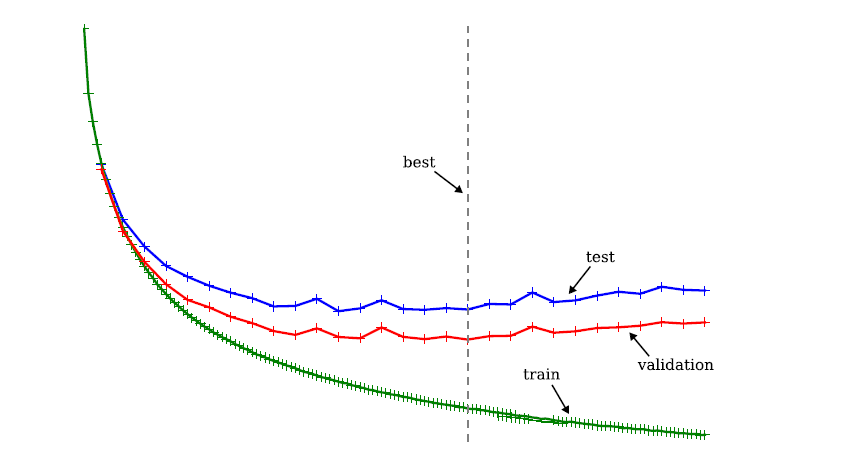
\includegraphics[scale=.45]{imagenes/appendices/appA_overfitting.PNG}
    \caption{Example of early stopping analysis using validation data~\cite{seqlab:Graves2012-385}.}
    \label{fig:earlyStopppingExample}
\end{figure}

One solution that helps to address the overfitting issue is to use a small portion of the 
training set as a validation set to include an \textbf{early stopping criteria}. This 
validation set is not used to train the network but to perform validation steps every certain 
amount of training steps. Then, the loss values for the validation steps are used to decide 
when to stop training. For example, Figure~\ref{fig:earlyStopppingExample} shows the losses 
over all three data sets (train, validation, test) through the training process Then, we can 
detect that the best weight values are found just before the validation loss stops its 
decreasing tendency and start increasing again (where the “best” stripped vertical line is 
placed). There are other techniques to reduce overfitting known as regularizers based on 
input noise~\cite{appendix:an1996effects, appendix:koistinen1991kernel, appendix:bishop1995neural} 
or weight noise~\cite{appendix:murray1994enhanced,appendix:jim1996analysis}.

Though most of the performance of ANNs relies on learnable parameters (such as layers’ weights), 
there are other parameters that can be set manually to improve the model’s performance, also 
known as \textbf{hyperparameters}. Some hyperparameters could be the number of hidden layers, 
the number of hidden units per layer, the learning rate, among others.

Lastly, it is also important to understand how the network input is represented. When we 
mention the \textbf{input representation}, we refer to the representation of the information 
required to predict the outputs, such as the input vector or the network weights. One 
procedure is input standardisation, which consists of normalizing the components of the input 
vectors to have mean 0 and standard deviation 1 over the training set. This standardization 
does not alter the information but helps to improve performance by limiting the values of the 
input vector to a more suitable range for a standard activation function~\cite{appendix:lecun1998efficient}. 
Note that the validation set and test set have to be standardised using the same distribution 
used for the training set. 

Another procedure is \textbf{weight initialisation}, which helps gradient descent to 
\textit{“break symmetry”} between units~\cite{appendix:lecun1998efficient} and avoid training 
divergence. Weight initialisation then is to initialise weights with either a random 
distribution in the range of small values or a Gaussian distribution with mean 0 and 
standard deviation 0.1.

After reviewing the fundamental concepts needed to understand how neural networks are 
structured and trained, we will review two neural networks architectures used in this work: 
Recurrent Neural Networks and Convolutional Neural Networks.

\section{Recurrent Neural Networks}
\label{appendix:recurrentNN}
A Recurrent Neural Network (RNN) is a generalization of traditional feedforward Neural 
Networks that allows cyclical connections~\cite{seqlab:Graves2012-385}. While MLPs can only 
map from input to output vectors, RNNs can map the entire history of previous inputs to an 
output. Hence, RNN connections allow the network to have “memory” of previous inputs, thus 
influencing the network output. Furthermore, RNNs are more fit for tasks involving sequence 
data, such as text or audio. An example of a RNN architecture can be seen in Figure 1.

\begin{figure}[!h]
    \centering
    
\includegraphics[scale=.45]{imagenes/insertImage.png}
    \caption{Recurrent Neural Network architecture example.}
    \label{fig:recurrentNN}
\end{figure}

A standard RNN computes the \textbf{forward pass} the same way as an MLP with a single hidden 
layer, with the difference that the activations arrive at the hidden layer from both the 
current external input and the hidden layer activations from the previous time step. Given a 
sequence of inputs $(x_1,\ldots,x_T)$, with $T$ the input length, the forward pass for an RNN 
with $I$ input units and $H$ hidden units is computed using the following formula:

\begin{equation} \label{eq:hiddenStateRNN}
    a_h^t = \sum_{i=1}^I w_{ih} \; x_i^t + \sum_{h'=1}^H w_{h'h} \; b_{h'}^{t-1}	
\end{equation}

where $x_i^t$ denotes the value of input $i$, $a_j^t$ is the network input to unit $j$, and 
$b_j^t$ is the activation unit of unit $j$, all three at time t. Then, the non-linearity $h$ 
is applied the same way as for an MLP, where functions such as the sigmoid function or 
softmax function are again a common choice:

\begin{equation} \label{eq:activationRNN}
    b_h^t = \theta_h(a_h^t)
\end{equation}

The entire learning process for RNNs is then summarized as a recursive application of the 
Equations~\ref{eq:hiddenStateRNN} and~\ref{eq:activationRNN}, starting at $t =1$. Since 
initial values $b_i^0$ are needed, they can be initialized using the same weight 
initialization methods mentioned above. The output units $a_k$ can be calculated at the same way 
as the hidden activations:

\begin{equation} \label{eq:hiddenStateRNN}
    a_k^t = \sum_{h=1}^H w_{hk} \; b_{h}^{t}	
\end{equation}

Then, the final activation function also depends on the task involved. For connection 
temporal classification (CTC) tasks, such as sequence labeling or translation, it is common 
to use the softmax function~\cite{appendix:graves2006connectionist}. The CTC loss function is 
used, that is defined as the negative log probability of correctly labelling all examples in 
the training set.

The \textbf{backward pass} can be performed using a backpropagation through time (BPTT) 
algorithm~\cite{appendix:williams1995gradient, semPar:werbos1990}, which is an algorithm 
based on the standard backpropagation process but adapted to RNNs. The BPTT algorithm also 
consists of a repeated application of the chain rule, with the difference that, aside from 
the output layer, the loss function also depends on the activation of the hidden layer 
through its influence on the hidden layer at the next timestep. The derivatives can be 
calculated using the same procedure described in the Learning process subsection, but taking 
into consideration that the same weights are being reused at every timestep.

Since the classical RNN architecture only looks to past information, the \textbf{Bidirectional 
Recurrent Neural Network} (BRNN) was proposed to also include future 
context~\cite{appendix:SchusterP97}. The BRNN’s structure consists of two separate recurrent 
hidden layers, both connected to the same output layer. This idea allows a forwards and 
backwards training sequence, where the layer that performs the backward training receives the 
input sequence in the opposite direction. The output layer is not updated until both hidden 
layers have processed the entire input sequence.

\subsection{Long Short-Term Memory}
Though RNNs work well with short sentences, their performance decreases with long sentences 
that involve long term dependencies due to the \textbf{vanishing gradient} 
problem~\cite{seqlab:HochreiterS97, appendix:hochreiter2001gradient}, which occurs when the 
influence of the given input on the hidden layer (and therefore on the network output), 
either decays or explodes exponentially through the recurrent connections. In order to 
address this issue, the \textbf{Long Short-Term Memory} (LSTM) model~\cite{seqlab:HochreiterS97} 
was proposed. The LSTM model allows models to perform on tasks which require long range 
temporal dependencies, such as Sequence Labeling~\cite{seqlab:HuangXY15, seqlab:MaH16}, 
Machine Translation~\cite{nlToSparql:WuSCLNMKCGMKSJL16} or Summarization~\cite{appendix:MahasseniLT17}. 
As per RNNs, the LSTM also has a bidirectional variant, also known as 
BiLSTM~\cite{appendix:graves2005framewise,appendix:ChenC04a,appendix:ThireouR07}. 

An LSTM network is similar to a standard RNN, except that the summations units in the hidden 
layer are replaced by \textbf{memory blocks}, as shown in Figure~\ref{fig:oneCellLSTM}. This 
structure allows the memory cells to store and access information over long periods of time, 
thereby reducing the effects of the vanishing gradient problem.

\begin{figure}[!h]
    \centering
    
\includegraphics[scale=.45]{imagenes/insertImage.png}
    \caption{LSTM memory block with one cell}
    \label{fig:oneCellLSTM}
\end{figure}

The following equations presented below are the formulas used to perform the forward pass 
evaluation over an LSTM with a single memory block for a timestep $t$. For multiple blocks 
the computations are repeated for each block. The values of $w_{ij}$, $a_j^t$ and $b_j^t$ 
have the same definition used before. 

First, the \textbf{Input Gates}, denoted as $a_\iota^t$~\ref{eq:inputHidden} and 
$b_\iota^t$~\ref{eq:inputActivation}. The number of inputs 
is denoted by $I$, the number of cells in the hidden layer is $H$ and the number of memory 
cells is $C$. The gate activation function $f$ most commonly used is the sigmoid function, so 
the gate activations are between 0 (gate closed) and 1 (gate open). The weight $w_{c\iota}$ 
represent the peephole weight from cell $c$ to the input gate. The state of the cell $c$ at 
time $t$ is denoted as $s_c^t$, which is calculated using Equation~\ref{eq:cellActivation}.

\begin{equation} \label{eq:inputHidden}
    a_\iota^t = \sum_{i=1}^I w_{i\iota} \; x_i^t + \sum_{h=1}^H w_{h\iota} \; b_h^{t-1} + \sum_{c=1}^C w_{c\iota} \; s_c^{t-1}
\end{equation}
\begin{equation} \label{eq:inputActivation}
    b_\iota^t = f(a_\iota^t)
\end{equation}

Then, the \textbf{Forget Gates}, denoted as $a_\phi^t$~\ref{eq:forgetHidden} and 
$b_\phi^t$~\ref{eq:forgetActivation}. The weight $w_{c\phi}$ represents the peephole weight 
from cell $c$ to the forget gate. Besides that, other symbols are equivalent to those 
mentioned for the input gate.

\begin{equation} \label{eq:forgetHidden}
    a_\phi^t = \sum_{i=1}^I w_{i\phi} \; x_i^t + \sum_{h=1}^H w_{h\phi} \; b_h^{t-1} + \sum_{c=1}^C w_{c\phi} \; s_c^{t-1}
\end{equation}
\begin{equation} \label{eq:forgetActivation}
    b_\phi^t = f(a_\phi^t)
\end{equation}

The \textbf{Cells}, denoted as $a_c^t$~\ref{eq:cellHidden} and $s_c^t$~\ref{eq:cellActivation}. The 
cell input activation function $g$ is usually hyperbolic tangent or sigmoid.

\begin{equation} \label{eq:cellHidden}
    a_c^t = \sum_{i=1}^I w_{ic} \; x_i^t + \sum_{h=1}^H w_{hc} \; b_h^{t-1}
\end{equation}
\begin{equation} \label{eq:cellActivation}
    s_c^t = b_\phi^t \; s_c^{t-1} + b_\iota^t \; g(a_c^t)
\end{equation}

Next, the \textbf{Outputs Gates}, denoted as $a_\omega^t$~\ref{eq:outputHidden} and 
$b_\omega^t$~\ref{eq:outputActivation}. The weight $w_{c\omega}$ represent the peephole w
eight from cell $c$ to the output gate.

\begin{equation} \label{eq:outputHidden}
    a_\omega^t = \sum_{i=1}^I w_{i\omega} \; x_i^t + \sum_{h=1}^H w_{h\omega} \; b_h^{t-1} + \sum_{c=1}^C w_{c\omega} \; s_c^{t-1}
\end{equation}
\begin{equation} \label{eq:outputActivation}
    b_\omega^t = f(a_\omega^t)
\end{equation}

Finally, the \textbf{Cell Outputs}, denoted as $b_c^t$~\ref{eq:cellOutput}. The cells outputs $b_c^t$ 
are the only ones connected to the other blocks in the layer. The index h is used to refer 
to cell outputs from other blocks in the hidden layer, if they exist. As per $g$, the output 
activation function $h$ is usually hyperbolic tangent or sigmoid, though sometimes the 
identity function can be used. 

\begin{equation} \label{eq:cellOutput}
    b_c^t = b_\omega^t \; f(s_c^t)
\end{equation}


\section{Convolutional Neural Networks}
\label{appendix:convolutionalNN}
The creation of \textbf{Convolutional Neural Networks} (CNNs) responds to the need to process 
certain types of data: images~\cite{appendix:OSheaN15}. Traditional ANNs do not perform well 
when processing images since its architecture does not properly support the computational 
complexity that involves processing large images as input. Whereas a 32$\times$32 image will 
be no problem to an traditional ANN, since it will require only 1024 parameters for a single 
neuron, images tend to have more resolution. On a higher scale, an image of 1024$\times$1024 
will instead require 1,048,576 parameters, which is a substantial increase. Moreover, if we 
consider colored images (RGB), a 1024$\times$1024 RGB image would require 3,145,728 
parameters. There is then a noticeable drawback of using standard feed-forward models where 
nodes are often connected to each node from the previous layer.

Convolutional Neural Networks share many similarities with standard ANNs in the way that both 
are composed of a set of neurons that are capable of learning, where each neuron receives an 
input and performs many operations, which commonly is a scalar product followed by an 
activation function. The difference resides in that CNNs are based on the idea that the input 
is shaped as an image. This idea allows the CNN architecture to adapt to this specific type 
of data. Then, a CNN architecture is built using three different types of layers: 
convolutional layers, pooling layers and fully-connected layers (same layers used in 
traditional ANNs). Additionally, each layer is organised into three dimensions: the spatial 
dimension (width and height) and the number of channels (also as known as depth, which is not 
the same as the number of layers). An example of a CNN architecture for pattern image 
classification is shown in Figure~\ref{fig:convNet}.

\begin{figure}[!h]
    \centering
    
\includegraphics[scale=.45]{imagenes/insertImage.png}
    \caption{Convolutional Neural Network for pattern image classification.}
    \label{fig:convNet}
\end{figure}

\subsection{Convolutional layer}
A \textbf{convolution layer} is the central component of CNNs, which determines the output of 
neurons using calculations based on local regions of the input. This type of layer is based on 
learnable kernels, which define local convolution operations over the input vector. A 
convolution consists of the scalar product for each value in a kernel of dimension M$\times$N 
over a local region with the same size as the kernel used:

\begin{equation} \label{eq:convolution}
    (X \ast w)_{i, j} = \sum_{m=1}^M \sum_{n=1}^{N} X_{m, n} \cdot w_{i-m, j-n}
\end{equation}

\begin{figure}[!h]
    \centering
    
\includegraphics[scale=.45]{imagenes/insertImage.png}
    \caption{Convolutional Neural Network for pattern image classification.}
    \label{fig:convNet}
\end{figure}

For example, in Figure~\ref{fig:convolutionPoolingExample} the convolution is being applied 
over a 3$\times$3 pooled vector, which is the size of the kernel $w$, that is, the local 
region of the entire input vector $X$. Though these kernels usually have a small spatial 
dimensionality, they are spread along the whole input vector. Besides kernel dimension, an 
application of padding over the input vector is also possible, which is the process of 
padding the border of the input with zeros. \textbf{Padding} controls both the dimensionality 
of the output volumes and gives more relevance to the input borders. Lastly, the 
\textbf{stride} is the amount of spaces the kernel is moved between each convolution. By 
setting a stride greater than 1, it is possible to reduce the amount of overlap and thus 
reduce the dimension of the activation output.

\begin{figure}[!h]
    \centering
    
\includegraphics[scale=.45]{imagenes/insertImage.png}
    \caption{Convolution operation example.}
    \label{fig:convolutionPoolingExample}
\end{figure}

Let $N$ be the size of a input vector of size N$\times$N, $F$ the kernel F$\times$F dimension, 
$P$ the padding size, and $S$ the stride value; the final dimension of the output volume will 
be $\left\lfloor \frac{N - F + 2P}{S} + 1 \right\rfloor$. Note that, in the same way an image can be 
represented in 3 dimensions, the kernel can be extended to a third dimension by increasing 
the \textbf{number of channels}, thus giving control over the output depth of the 
convolutional layer. The number of channels, stride and padding are hyperparameters that can 
be optimised. 

Kernel values are the trainable parameters which a CNN can tuned in through the same type 
of learning process ANNs perfom. The composition of convolutional layers allows to reduce the 
dimensionality of a Neural Network in terms of learnable parameters, based on the assumption 
of parameter sharing. This assumption says that \textit{“if one region is useful to compute at 
a set spatial region, then it is likely to be useful in another region”}. The constraints of 
each activation within the output volume to the same weights and bias means a significant 
decrease in the number of parameters used in a convolution layer. Then, the backward pass for 
each neuron in the output represents the overall gradient across channels, where only a 
single set of weights is updated.

After the application of the convolution, an activation function is applied over the output 
volume. The most common choice is the rectified linear unit (ReLu) which is an elementwise 
function that given a certain threshold $\alpha$ will set all values less than $\alpha$ to 0 .

\subsection{Pooling layer}
A pooling layer aims to reduce the volume of an input representation with the purposes of 
reducing the computational complexity of the model. After each activation from a convolutional 
layer, a pooling layer can be applied to scale its dimensionality through a reducing function. 
The most common type of pooling is the max-pooling layer, which is a kernel that applies a 
MAX reduction on a local region as per a convolutional kernel. Other examples are average 
pooling, or general pooling that applies average reduction and $L_1$/$L_2$ normalization 
respectively.

Though pooling layers also include settings such as kernel size, stride or number of channels, 
they do not add learnable parameters. However, they do influences in the backward pass to 
calculate the gradients. Lastly, it is recommended to keep a low stride and kernel size since 
its application could affect negatively performance if large values are used.

\subsection{Common architectures}
As mentioned before, a CNN architecture is commonly built with an input layer, which receives 
the values of the image, followed by various stacked convolutional layers, each one followed 
by pooling layers, and a final stack of fully-connected layers. However, defining exactly the 
amount of layers to use is not a simple task. In fact, most of the literature is based on 
standard architectures that have shown good results on certain image processing tasks.

Among the most popular architectures, ImageNet~\cite{appendix:KrizhevskySH12} is a Deep 
Convolutional Network with five convolutional layers, some followed by max-pooling layers, 
followed by two fully-connected layers. Another example is ResNet~\cite{appendix:HeZRS16}, 
which includes \textbf{residual connections} that aim to reduce the vanishing gradient 
problem that a very dense convolutional network can suffer. The main principle of residual 
connections is to create connections between non-adjacent layers that skip a certain 
amount of layers.
\chapter{Question Answering Dataset}
\label{appendix:qaDataset}
We provide more details on the data used for the training and validation of our system.

\section{Normalized Dataset Format}
\label{appendix:qaDataset/normalizedFormat}
As mentioned in the \textit{Experimental Design} chapter, we proposed a dataset format so the process 
of generating the Query Template dataset and the Sequence Labeling datasets could be simplified. This 
normalized format is also used for the other test datasets (QALD-7 and WikiSPARQL). In 
Listing~\ref{lst:normalizedDatasetExample} we can see an example of what information each case contains:

\begin{sparqlcode}[%
    caption={Example of one \LCQuADtwo{} case following our proposed normalized format.}, 
    label={lst:normalizedDatasetExample}]
    "question_id": 30226,
    "natural_language_question": "Did Alexander Hamilton practice law?",
    "query_answer": [
        {
            "query_id": 0,
            "sparql_query": 
                "ASK WHERE { wd:Q178903 wdt:P106 wd:Q40348 }",
            "entities": [ 
                {"label": "Alexander Hamilton", "entity": "wd:Q178903"},
                {"label": "lawyer", "entity": "wd:Q40348"}
            ],
            "slots": [
                {"slot": "<sbj_1>", "label": "Alexander Hamilton"},
                {"slot": "<obj_1>", "label": "lawyer"}
            ],
            "sparql_template": "ASK WHERE { <sbj_1> wdt:P106 <obj_1> }"
        }
    ]
\end{sparqlcode}

\begin{itemize}
    \item \textbf{Question ID}: the unique identifier of the question; for \LCQuADtwo{} we decided to 
    treat each verbalized and paraphrased version of the normalized question as a separate case. 
    Verbalized cases are then numbered from $0$ to $30,225$, and paraphrased cases from $30,226$ to $60,451$.
    \item \textbf{Natural Language Question}: the question text (verbalized or paraphrased version).
    \item \textbf{Query Answer}: a list of possible SPARQL query valid responses. We allow more than 
    one possible query since for each question there are many ways to reach the expected answer (for 
    example, \dquotesit{What is the biggest country?} may refer to population, area, etc.; however in 
    this work we only have one SPARQL query per case). Each query answer case has the following fields:
    \begin{itemize}
        \item \textbf{Query ID}: unique identifier to identify query answers for the same question.
        \item \textbf{SPARQL query}: the SPARQL query string.
        \item \textbf{Entities}: list of expected annotations of the entities being used in the 
        SPARQL query answer. Each annotation contains the entity URL and the label of the question 
        associated with that entity.
        \item \textbf{Slots}: list of expected slots to use for the Slot Filling system. Each slot 
        contains the associated label in the question and its corresponding placeholder in the Query 
        Template.
        \item \textbf{SPARQL Template}: the Query Template derived from the SPARQL query.
    \end{itemize}
\end{itemize}

\section{LC-QuAD 2 base templates}
\label{appendix:qaDataset/baseTemplates}
In the Results chapter we displayed some analysis based on the 22 base templates used for building 
the \LCQuADtwo{} dataset~\cite{dataset:lcquad2-DubeyBA019}. According to each base template structure, 
we established which cases are considered \textbf{complex cases}, which allows us to estimate the 
percentage of complex questions this dataset contains. A base template is considered a \textit{complex 
case} if it includes any of the following operations: (1) counting, (2) filtering, (3) ordering, 
(4) use of strings or numbers,(5) use of property statements, or (6) returns more than one variable. 

Next, we present a brief overview of each one of these base templates along with a representative 
example from the dataset:

\begin{enumerate}
    \item \textbf{ask\_one\_fact}: ASK query with one query triple.
    \begin{itemize}
        \item Example: \textit{Did Alexander Hamilton practice law?}
        \item Query:\\
        \mbox{}\\
        \begin{sparqlcode}[]
ASK WHERE { 
    wd:Q178903 wdt:P106 wd:Q40348 
}
        \end{sparqlcode}
    \end{itemize}

    \item \textbf{ask\_one\_fact\_with\_filter}: ASK query with one query triple and a numeric filter 
    operation (either less than, equal, or greater than).
    \begin{itemize}
        \item Example: \textit{Does the standard molar entropy of silver equal 34.08?}
        \item Query:\\
        \mbox{}\\
        \begin{sparqlcode}[]
ASK WHERE { 
    wd:Q1090 wdt:P3071 ?obj filter(?obj = 34.08) 
}
        \end{sparqlcode}
    \end{itemize}

    \item \textbf{ask\_two\_facts}: ASK query with two query triples. Note that the same subject 
    and property are used in both query triples.
    \begin{itemize}
        \item Example: \textit{Was William Henry Harrison both a United States senator and Governor of 
        Indiana?}
        \item Query:\\
        \mbox{}\\
        \begin{sparqlcode}[]
ASK WHERE { 
    wd:Q11869 wdt:P39 wd:Q16147601 . 
    wd:Q11869 wdt:P39 wd:Q13217683 
}
        \end{sparqlcode}
    \end{itemize}

    \item \textbf{count\_one\_fact\_object}: SELECT query with COUNT operation from one query triple. 
    Count the number of objects that match the query triple.
    \begin{itemize}
        \item Example: \textit{How many Latin conjugations are there?}
        \item Query:\\
        \mbox{}\\
        \begin{sparqlcode}[]
SELECT (COUNT(?obj) AS ?value ) WHERE { 
    wd:Q397 wdt:P5206 ?obj 
}
        \end{sparqlcode}
    \end{itemize}

    \item \textbf{count\_one\_fact\_subject}: SELECT query with COUNT operation from one query triple. 
    Count the number of subjects that match the query triple.
    \begin{itemize}
        \item Example: \textit{What is the number of spore print colors for olive?}
        \item Query:\\
        \mbox{}\\
        \begin{sparqlcode}[]
SELECT (COUNT(?sbj) AS ?value ) WHERE { 
    ?sbj wdt:P787 wd:Q864152 
}
        \end{sparqlcode}
    \end{itemize}

    \item \textbf{rank\_instance\_of\_type\_one\_fact}: SELECT query with two query triples with 
    sorting and limit. The first query triple always uses the property instance of (wdt:P31). 
    Ordering might vary (ascending or descending).
    \begin{itemize}
        \item Example: \textit{What battery power station has the highest amount of energy storage 
        capacity?}
        \item Query:\\
        \mbox{}\\
        \begin{sparqlcode}[]
SELECT ?ent WHERE { 
    ?ent wdt:P31 wd:Q810924 . 
    ?ent wdt:P4140 ?obj 
} ORDER BY DESC(?obj) LIMIT 5
        \end{sparqlcode}
    \end{itemize}
    
    \item \textbf{rank\_max\_instance\_of\_type\_two\_facts}: SELECT query with three query triples using 
    sorting and limit. The first query triple always uses the property instance of (wdt:P31). 
    Descending ordering is used to get the maximum value.
    \begin{itemize}
        \item Example: \textit{What is the largest village in Muchinigi Puttu?}
        \item Query:\\
        \mbox{}\\
        \begin{sparqlcode}[]
SELECT ?ent WHERE { 
    ?ent wdt:P31 wd:Q532 . 
    ?ent wdt:P2046 ?obj . 
    ?ent wdt:P131 wd:Q11107378 
} ORDER BY DESC(?obj) LIMIT 5
        \end{sparqlcode}
    \end{itemize}
    
    \item \textbf{rank\_min\_instance\_of\_type\_two\_facts}: Same as the previous base template but with 
    ascending ordering to get the minimum value.
    \begin{itemize}
        \item Example: \textit{What is the name of a manned spacecraft in low Earth orbit with 
        smallest periapsis?}
        \item Query:\\
        \mbox{}\\
        \begin{sparqlcode}[]
SELECT ?ent WHERE { 
    ?ent wdt:P31 wd:Q7217761 . 
    ?ent wdt:P2244 ?obj . 
    ?ent wdt:P522 wd:Q663611
} ORDER BY ASC(?obj) LIMIT 5
        \end{sparqlcode}
    \end{itemize}
    
    \item \textbf{select\_object\_instance\_of\_type}: SELECT query with two query triples. The first 
    query triple always uses the property instance of (wdt:P31). Return the entities that are the 
    object of the first query triple.
    \begin{itemize}
        \item Example: \textit{What is the prefecture of Hiroshima in Japan?}
        \item Query:\\
        \mbox{}\\
        \begin{sparqlcode}[]
SELECT DISTINCT ?obj WHERE { 
    wd:Q34664 wdt:P131 ?obj . 
    ?obj wdt:P31 wd:Q50337 
}
        \end{sparqlcode}
    \end{itemize}
    
    \item \textbf{select\_object\_using\_one\_statement\_property}: SELECT query with three query 
    triples. Uses one property statement and one property qualifier. 
    \begin{itemize}
        \item Example: \textit{When did Louis XVIII of France, husband of Marie Josephine of Savoy, 
        die?}
        \item Query:\\
        \mbox{}\\
        \begin{sparqlcode}[]
SELECT ?value WHERE { 
    wd:Q7750 p:P26 ?s . 
    ?s ps:P26 wd:Q231844 . 
    ?s pq:P582 ?value
}
        \end{sparqlcode}
    \end{itemize}
    
    \item \textbf{select\_one\_fact\_object}: SELECT query with one query triple. Return the entities 
    that are the subject of that query triple.
    \begin{itemize}
        \item Example: \textit{Which are the characters for La Malinche?}
        \item Query:\\
        \mbox{}\\
        \begin{sparqlcode}[]
SELECT DISTINCT ?answer WHERE { 
    ?answer wdt:P674 wd:Q230314
}
        \end{sparqlcode}
    \end{itemize}
    
    \item \textbf{select\_one\_fact\_subject}: SELECT query with one query triple. Return the entities 
    that are the object of that query triple.
    \begin{itemize}
        \item Example: \textit{Which is the electric charge for antihydrogen?}
        \item Query:\\
        \mbox{}\\
        \begin{sparqlcode}[]
SELECT DISTINCT ?answer WHERE { 
    wd:Q216121 wdt:P2200 ?answer
}
        \end{sparqlcode}
    \end{itemize}
    
    \item \textbf{select\_one\_qualifier\_value\_and\_object\_using\_one\_statement\_property}: SELECT query 
    with three query triples. Uses one property statement and one property qualifier. Only one entity 
    used for the first query triple.
    \begin{itemize}
        \item Example: \textit{What grant did Konrad Lorenz win, and who won it with him?}
        \item Query:\\
        \mbox{}\\
        \begin{sparqlcode}[]
SELECT ?value1 ?obj WHERE { 
    wd:Q78496 p:P166 ?s . 
    ?s ps:P166 ?obj . 
    ?s pq:P1706 ?value1 . 
}
        \end{sparqlcode}
    \end{itemize}
    
    \item \textbf{select\_one\_qualifier\_value\_using\_one\_statement\_property}: SELECT query with three 
    query triples. Uses one property statement and one property qualifier. Two entities used for 
    building each query, where the second entity was used as the object of the property qualifier 
    triple.
    \begin{itemize}
        \item Example: \textit{What role did Theodore Roosevelt occupy after William McKinley?}
        \item Query:\\
        \mbox{}\\
        \begin{sparqlcode}[]
SELECT ?obj WHERE { 
    wd:Q33866 p:P39 ?s . 
    ?s ps:P39 ?obj . 
    ?s pq:P1365 wd:Q35041 
}
        \end{sparqlcode}
    \end{itemize}
    
    \item \textbf{select\_subject\_instance\_of\_type}: SELECT query with two query triples. The first 
    query triple always uses the property instance of (wdt:P31). Return the entities that are the 
    subject of the first query triple.
    \begin{itemize}
        \item Example: \textit{Which irresistible illness is caused by Staphylococcus aureus?}
        \item Query:\\
        \mbox{}\\
        \begin{sparqlcode}[]
SELECT DISTINCT ?sbj WHERE { 
    ?sbj wdt:P828 wd:Q188121 . 
    ?sbj wdt:P31 wd:Q18123741 
}
        \end{sparqlcode}
    \end{itemize}
    
    \item \textbf{select\_subject\_instance\_of\_type\_contains\_word}: SELECT query with two query triples. 
    The first query triple always uses the property instance of (wdt:P31). The second query triple 
    also includes a filter over the string value to check whether the target word is contained in 
    this string (includes filtering for the English language).
    \begin{itemize}
        \item Example: \textit{What is the title of a human that contains the word vitellius in their 
        name.}
        \item Query:\\
        \mbox{}\\
        \begin{sparqlcode}[]
SELECT DISTINCT ?sbj ?sbj_label WHERE { 
    ?sbj wdt:P31 wd:Q5 . 
    ?sbj rdfs:label ?sbj_label . 
    FILTER(CONTAINS(lcase(?sbj_label), 'vitellius')) . 
    FILTER (lang(?sbj_label) = 'en') 
} LIMIT 25
        \end{sparqlcode}
    \end{itemize}
    
    \item \textbf{select\_subject\_instance\_of\_type\_starts\_with}: SELECT query with two query triples. 
    The first query triple always uses the property instance of (wdt:P31). The second query triples 
    also includes a filtering over the string value to check whether this string starts with a target 
    letter (including filtering for the  English language).
    \begin{itemize}
        \item Example: \textit{What are the video games which start with the letter W?}
        \item Query:\\
        \mbox{}\\
        \begin{sparqlcode}[]
SELECT DISTINCT ?sbj ?sbj_label WHERE { 
    ?sbj wdt:P31 wd:Q7058673 . 
    ?sbj rdfs:label ?sbj_label . 
    FILTER(STRSTARTS(lcase(?sbj_label), 'w')) . 
    FILTER (lang(?sbj_label) = 'en') 
} LIMIT 25
        \end{sparqlcode}
    \end{itemize}
    
    \item \textbf{select\_two\_answers}: SELECT query with two query triples. Return two variables 
    (also known as double intention), with each one being the object of each query triple.
    \begin{itemize}
        \item Example: \textit{Where was Jane Austen born and where did she die?}
        \item Query:\\
        \mbox{}\\
        \begin{sparqlcode}[]
SELECT ?ans_1 ?ans_2 WHERE { 
    wd:Q36322 wdt:P19 ?ans_1 . 
    wd:Q36322 wdt:P20 ?ans_2 
}
        \end{sparqlcode}
    \end{itemize}
    
    \item \textbf{select\_two\_facts\_left\_subject}: SELECT query with two query triples.
    \begin{itemize}
        \item Example: \textit{Who were the creators of The Late Awesome Planet Soil?}
        \item Query:\\
        \mbox{}\\
        \begin{sparqlcode}[]
SELECT ?answer WHERE { 
    wd:Q22081649 wdt:P144 ?obj . 
    ?obj wdt:P50 ?answer
}
        \end{sparqlcode}
    \end{itemize}
    
    \item \textbf{select\_two\_facts\_right\_subject}: SELECT query with two query triples. Similar to 
    the previous template (in fact we could not find any difference between both cases).
    \begin{itemize}
        \item Example: \textit{What time zone is Arizona State University in?}
        \item Query:\\
        \mbox{}\\
        \begin{sparqlcode}[]
SELECT ?answer WHERE { 
    wd:Q670897 wdt:P17 ?obj . 
    ?obj wdt:P421 ?answer
}
        \end{sparqlcode}
    \end{itemize}
    
    \item \textbf{select\_two\_facts\_subject\_object}: SELECT query with two query triples. Uses one 
    entity in the subject of the first query triple, and another one in the object of the second 
    query triple.
    \begin{itemize}
        \item Example: \textit{What lake of Sao Jorge island has the tributary Curoca River?}
        \item Query:\\
        \mbox{}\\
        \begin{sparqlcode}[]
SELECT ?answer WHERE { 
    wd:Q743362 wdt:P206 ?answer . 
    ?answer wdt:P974 wd:Q10361834
}
        \end{sparqlcode}
    \end{itemize}
    
    \item \textbf{select\_two\_qualifier\_values\_using\_one\_statement\_property}: SELECT query 
    with four query triples. Uses one property statement and two property qualifiers. Return the two object 
    values of each query triple using a property qualifier.
    \begin{itemize}
        \item Example: \textit{Give me the year and name of the person with whom Bob Barker shared the 
        MTV Movie Award for Best Fight.}
        \item Query:\\
        \mbox{}\\
        \begin{sparqlcode}[]
SELECT ?value1 ?value2 WHERE { 
    wd:Q381178 p:P166 ?s . 
    ?s ps:P166 wd:Q734036 . 
    ?s pq:P585 ?value1 . 
    ?s pq:P1706 ?value2 
}
        \end{sparqlcode}
    \end{itemize}
    
\end{enumerate}
 % opcionales

\end{document}
